\documentclass[a4paper]{article}

\def\npart {IB}
\def\nterm {Michaelmas}
\def\nyear {2015}
\def\nlecturer {S. J. Wadsley}
\def\ncourse {Linear Algebra}
\def\nofficial{https://www.dpmms.cam.ac.uk/~sjw47/LinearAlgebraM15.pdf}

% Imports
\ifx \nextra \undefined
  \usepackage[pdftex,
    hidelinks,
    pdfauthor={Dexter Chua},
    pdfsubject={Cambridge Maths Notes: Part \npart\ - \ncourse},
    pdftitle={Part \npart\ - \ncourse},
  pdfkeywords={Cambridge Mathematics Maths Math \npart\ \nterm\ \nyear\ \ncourse}]{hyperref}
  \title{Part \npart\ - \ncourse}
\else
  \usepackage[pdftex,
    hidelinks,
    pdfauthor={Dexter Chua},
    pdfsubject={Cambridge Maths Notes: Part \npart\ - \ncourse\ (\nextra)},
    pdftitle={Part \npart\ - \ncourse\ (\nextra)},
  pdfkeywords={Cambridge Mathematics Maths Math \npart\ \nterm\ \nyear\ \ncourse\ \nextra}]{hyperref}

  \title{Part \npart\ - \ncourse \\ {\Large \nextra}}
\fi

\author{Lectured by \nlecturer \\\small Notes taken by Dexter Chua}
\date{\nterm\ \nyear}

\usepackage{alltt}
\usepackage{amsfonts}
\usepackage{amsmath}
\usepackage{amssymb}
\usepackage{amsthm}
\usepackage{booktabs}
\usepackage{caption}
\usepackage{enumitem}
\usepackage{fancyhdr}
\usepackage{graphicx}
\usepackage{mathtools}
\usepackage{microtype}
\usepackage{multirow}
\usepackage{pdflscape}
\usepackage{pgfplots}
\usepackage{siunitx}
\usepackage{tabularx}
\usepackage{tikz}
\usepackage{tkz-euclide}
\usepackage[normalem]{ulem}
\usepackage[all]{xy}

\pgfplotsset{compat=1.12}

\pagestyle{fancyplain}
\lhead{\emph{\nouppercase{\leftmark}}}
\ifx \nextra \undefined
  \rhead{
    \ifnum\thepage=1
    \else
      \npart\ \ncourse
    \fi}
\else
  \rhead{
    \ifnum\thepage=1
    \else
      \npart\ \ncourse\ (\nextra)
    \fi}
\fi
\usetikzlibrary{arrows}
\usetikzlibrary{decorations.markings}
\usetikzlibrary{decorations.pathmorphing}
\usetikzlibrary{positioning}
\usetikzlibrary{fadings}
\usetikzlibrary{intersections}
\usetikzlibrary{cd}

\newcommand*{\Cdot}{\raisebox{-0.25ex}{\scalebox{1.5}{$\cdot$}}}
\newcommand {\pd}[2][ ]{
  \ifx #1 { }
    \frac{\partial}{\partial #2}
  \else
    \frac{\partial^{#1}}{\partial #2^{#1}}
  \fi
}

% Theorems
\theoremstyle{definition}
\newtheorem*{aim}{Aim}
\newtheorem*{axiom}{Axiom}
\newtheorem*{claim}{Claim}
\newtheorem*{cor}{Corollary}
\newtheorem*{defi}{Definition}
\newtheorem*{eg}{Example}
\newtheorem*{fact}{Fact}
\newtheorem*{law}{Law}
\newtheorem*{lemma}{Lemma}
\newtheorem*{notation}{Notation}
\newtheorem*{prop}{Proposition}
\newtheorem*{thm}{Theorem}

\renewcommand{\labelitemi}{--}
\renewcommand{\labelitemii}{$\circ$}
\renewcommand{\labelenumi}{(\roman{*})}

\let\stdsection\section
\renewcommand\section{\newpage\stdsection}

% Strike through
\def\st{\bgroup \ULdepth=-.55ex \ULset}

% Maths symbols
\newcommand{\bra}{\langle}
\newcommand{\ket}{\rangle}

\newcommand{\N}{\mathbb{N}}
\newcommand{\Z}{\mathbb{Z}}
\newcommand{\Q}{\mathbb{Q}}
\renewcommand{\H}{\mathbb{H}}
\newcommand{\R}{\mathbb{R}}
\newcommand{\C}{\mathbb{C}}
\newcommand{\Prob}{\mathbb{P}}
\renewcommand{\P}{\mathbb{P}}
\newcommand{\E}{\mathbb{E}}
\newcommand{\F}{\mathbb{F}}
\newcommand{\cU}{\mathcal{U}}
\newcommand{\RP}{\mathbb{RP}}
\newcommand{\CP}{\mathbb{CP}}

\newcommand{\ph}{\,\cdot\,}

\DeclareMathOperator{\sech}{sech}
\DeclareMathOperator{\cosech}{cosech}
\DeclareMathOperator{\cosec}{cosec}

\DeclareMathOperator{\covol}{covol}
\DeclareMathOperator{\vol}{vol}

\let\Im\relax
\let\Re\relax
\DeclareMathOperator{\Im}{Im}
\DeclareMathOperator{\Re}{Re}
\DeclareMathOperator{\im}{im}
\DeclareMathOperator{\image}{image}
\DeclareMathOperator{\Ann}{Ann}

\DeclareMathOperator*{\res}{res}
\DeclareMathOperator{\Res}{Res}
\DeclareMathOperator{\Ind}{Ind}

\DeclareMathOperator{\tr}{tr}
\DeclareMathOperator{\diag}{diag}
\DeclareMathOperator{\rank}{rank}
\DeclareMathOperator{\card}{card}
\DeclareMathOperator{\spn}{span}
\DeclareMathOperator{\adj}{adj}

\DeclareMathOperator{\erf}{erf}
\DeclareMathOperator{\erfc}{erfc}

\DeclareMathOperator{\ord}{ord}
\DeclareMathOperator{\Sym}{Sym}

\DeclareMathOperator{\sgn}{sgn}
\DeclareMathOperator{\orb}{orb}
\DeclareMathOperator{\stab}{stab}
\DeclareMathOperator{\ccl}{ccl}

\DeclareMathOperator{\lcm}{lcm}
\DeclareMathOperator{\hcf}{hcf}

\DeclareMathOperator{\Int}{Int}
\DeclareMathOperator{\id}{id}

\DeclareMathOperator{\betaD}{beta}
\DeclareMathOperator{\gammaD}{gamma}
\DeclareMathOperator{\Poisson}{Poisson}
\DeclareMathOperator{\binomial}{binomial}
\DeclareMathOperator{\multinomial}{multinomial}
\DeclareMathOperator{\Bernoulli}{Bernoulli}
\DeclareMathOperator{\like}{like}

\DeclareMathOperator{\var}{var}
\DeclareMathOperator{\cov}{cov}
\DeclareMathOperator{\bias}{bias}
\DeclareMathOperator{\mse}{mse}
\DeclareMathOperator{\corr}{corr}

\DeclareMathOperator{\otp}{otp}
\DeclareMathOperator{\dom}{dom}

\DeclareMathOperator{\Root}{Root}
\DeclareMathOperator{\supp}{supp}
\DeclareMathOperator{\rel}{rel}
\DeclareMathOperator{\Hom}{Hom}
\DeclareMathOperator{\Aut}{Aut}
\DeclareMathOperator{\Gal}{Gal}
\DeclareMathOperator{\Mat}{Mat}
\DeclareMathOperator{\End}{End}
\DeclareMathOperator{\Char}{char}
\DeclareMathOperator{\ev}{ev}
\DeclareMathOperator{\St}{St}
\DeclareMathOperator{\Lk}{Lk}
\DeclareMathOperator{\disc}{disc}
\DeclareMathOperator{\Isom}{Isom}
\DeclareMathOperator{\length}{length}
\DeclareMathOperator{\energy}{energy}
\DeclareMathOperator{\area}{area}
\DeclareMathOperator{\Syl}{Syl}
\DeclareMathOperator{\cl}{cl}
\DeclareMathOperator{\fix}{fix}

\newcommand{\GL}{\mathrm{GL}}
\newcommand{\SL}{\mathrm{SL}}
\newcommand{\PGL}{\mathrm{PGL}}
\newcommand{\PSL}{\mathrm{PSL}}
\newcommand{\PSU}{\mathrm{PSU}}
\newcommand{\Or}{\mathrm{O}}
\newcommand{\SO}{\mathrm{SO}}
\newcommand{\U}{\mathrm{U}}
\newcommand{\SU}{\mathrm{SU}}

\renewcommand{\d}{\mathrm{d}}
\newcommand{\D}{\mathrm{D}}

\tikzset{->/.style = {decoration={markings,
                                  mark=at position 1 with {\arrow[scale=2]{latex'}}},
                      postaction={decorate}}}
\tikzset{<-/.style = {decoration={markings,
                                  mark=at position 0 with {\arrowreversed[scale=2]{latex'}}},
                      postaction={decorate}}}
\tikzset{<->/.style = {decoration={markings,
                                   mark=at position 0 with {\arrowreversed[scale=2]{latex'}},
                                   mark=at position 1 with {\arrow[scale=2]{latex'}}},
                       postaction={decorate}}}
\tikzset{->-/.style = {decoration={markings,
                                   mark=at position #1 with {\arrow[scale=2]{latex'}}},
                       postaction={decorate}}}
\tikzset{-<-/.style = {decoration={markings,
                                   mark=at position #1 with {\arrowreversed[scale=2]{latex'}}},
                       postaction={decorate}}}

\tikzset{circ/.style = {fill, circle, inner sep = 0, minimum size = 3}}
\tikzset{mstate/.style={circle, draw, blue, text=black, minimum width=0.7cm}}

\definecolor{mblue}{rgb}{0.2, 0.3, 0.8}
\definecolor{morange}{rgb}{1, 0.5, 0}
\definecolor{mgreen}{rgb}{0.1, 0.4, 0.2}
\definecolor{mred}{rgb}{0.5, 0, 0}

\def\drawcirculararc(#1,#2)(#3,#4)(#5,#6){%
    \pgfmathsetmacro\cA{(#1*#1+#2*#2-#3*#3-#4*#4)/2}%
    \pgfmathsetmacro\cB{(#1*#1+#2*#2-#5*#5-#6*#6)/2}%
    \pgfmathsetmacro\cy{(\cB*(#1-#3)-\cA*(#1-#5))/%
                        ((#2-#6)*(#1-#3)-(#2-#4)*(#1-#5))}%
    \pgfmathsetmacro\cx{(\cA-\cy*(#2-#4))/(#1-#3)}%
    \pgfmathsetmacro\cr{sqrt((#1-\cx)*(#1-\cx)+(#2-\cy)*(#2-\cy))}%
    \pgfmathsetmacro\cA{atan2(#2-\cy,#1-\cx)}%
    \pgfmathsetmacro\cB{atan2(#6-\cy,#5-\cx)}%
    \pgfmathparse{\cB<\cA}%
    \ifnum\pgfmathresult=1
        \pgfmathsetmacro\cB{\cB+360}%
    \fi
    \draw (#1,#2) arc (\cA:\cB:\cr);%
}
\newcommand\getCoord[3]{\newdimen{#1}\newdimen{#2}\pgfextractx{#1}{\pgfpointanchor{#3}{center}}\pgfextracty{#2}{\pgfpointanchor{#3}{center}}}

\def\Xint#1{\mathchoice
   {\XXint\displaystyle\textstyle{#1}}%
   {\XXint\textstyle\scriptstyle{#1}}%
   {\XXint\scriptstyle\scriptscriptstyle{#1}}%
   {\XXint\scriptscriptstyle\scriptscriptstyle{#1}}%
   \!\int}
\def\XXint#1#2#3{{\setbox0=\hbox{$#1{#2#3}{\int}$}
     \vcenter{\hbox{$#2#3$}}\kern-.5\wd0}}
\def\ddashint{\Xint=}
\def\dashint{\Xint-}


\begin{document}
\maketitle
{\small
\noindent Definition of a vector space (over $\R$ or $\C$), subspaces, the space spanned by a subset. Linear independence, bases, dimension. Direct sums and complementary subspaces. \hspace*{\fill} [3]

\vspace{5pt}
\noindent Linear maps, isomorphisms. Relation between rank and nullity. The space of linear maps from $U$ to $V$, representation by matrices. Change of basis. Row rank and column rank.\hspace*{\fill} [4]

\vspace{5pt}
\noindent Determinant and trace of a square matrix. Determinant of a product of two matrices and of the inverse matrix. Determinant of an endomorphism. The adjugate matrix.\hspace*{\fill} [3]

\vspace{5pt}
\noindent Eigenvalues and eigenvectors. Diagonal and triangular forms. Characteristic and minimal polynomials. Cayley-Hamilton Theorem over $\C$. Algebraic and geometric multiplicity of eigenvalues. Statement and illustration of Jordan normal form.\hspace*{\fill} [4]

\vspace{5pt}
\noindent Dual of a finite-dimensional vector space, dual bases and maps. Matrix representation, rank and determinant of dual map.\hspace*{\fill} [2]

\vspace{5pt}
\noindent Bilinear forms. Matrix representation, change of basis. Symmetric forms and their link with quadratic forms. Diagonalisation of quadratic forms. Law of inertia, classification by rank and signature. Complex Hermitian forms.\hspace*{\fill} [4]

\vspace{5pt}
\noindent Inner product spaces, orthonormal sets, orthogonal projection, $V = W \oplus W^\bot$. Gram-Schmidt orthogonalisation. Adjoints. Diagonalisation of Hermitian matrices. Orthogonality of eigenvectors and properties of eigenvalues.\hspace*{\fill} [4]}

\tableofcontents
\setcounter{section}{-1}
\section{Introduction}
In IA Vectors and Matrices, we have learnt about vectors (and matrices) in a rather applied way. A vector was just treated as a ``list of numbers'' representing a point in space. We used these to represent lines, conics, planes and many other geometrical notions. A matrix is treated as a ``physical operation'' on vectors that stretches and rotates them. For example, we studied the properties of rotations, reflections and shears of space. We also used matrices to express and solve systems of linear equations. We mostly took a practical approach in the course.

In IB Linear Algebra, we are going to study vectors in an abstract setting. Instead of treating vectors as ``lists of numbers'', we view them as things we can add and scalar-multiply. We will write down axioms governing how these operations should behave, just like how we wrote down the axioms of group theory. Instead of studying matrices as an array of numbers, we instead look at linear maps between vector spaces abstractly.

In the course, we will, of course, prove that this abstract treatment of linear algebra is just ``the same as'' our previous study of ``vectors as a list of numbers''. Indeed, in certain cases, results are much more easily proved by working with matrices (as an array of numbers) instead of abstract linear maps, and we don't shy away from doing so. However, most of the time, looking at these abstractly will provide a much better fundamental understanding of how things work.

\section{Vector spaces}
\subsection{Definitions and examples}
\begin{notation}
  We will use $\F$ to denote an arbitrary field, usually $\R$ or $\C$.
\end{notation}

Intuitively, a vector space $V$ over a field $\F$ (or an $\F$-vector space) is a space with two operations:
\begin{itemize}
  \item We can add two vectors $\mathbf{v}_1, \mathbf{v}_2 \in V$ to obtain $\mathbf{v}_1 + \mathbf{v}_2 \in V$.
  \item We can multiply a scalar $\lambda \in \F$ with a vector $\mathbf{v}\in V$ to obtain $\lambda \mathbf{v} \in V$.
\end{itemize}

Of course, these two operations must satisfy certain axioms before we can call it a vector space. However, before going into these details, we first look at a few examples of vector spaces.

\begin{eg}\leavevmode
  \begin{enumerate}
    \item $\R^n = \{\text{column vectors of length }n\text{ with coefficients in }\R\}$ with the usual addition and scalar multiplication is a vector space.

      An $m\times n$ matrix $A$ with coefficients in $\R$ can be viewed as a linear map from $\R^m$ to $\R^n$ via $\mathbf{v} \mapsto A\mathbf{v}$.

      This is a motivational example for vector spaces. When confused about definitions, we can often think what the definition means in terms of $\R^n$ and matrices to get some intuition.

    \item Let $X$ be a set and define $\R^X = \{f: X\to \R\}$ with addition $(f + g)(x) = f(x) + g(x)$ and scalar multiplication $(\lambda f)(x) = \lambda f(x)$. This is a vector space.

      More generally, if $V$ is a vector space, $X$ is a set, we can define $V^X = \{f: X \to V\}$ with addition and scalar multiplication as above.
    \item Let $[a, b]\subseteq \R$ be a closed interval, then
      \[
        C([a, b], \R) = \{f\in \R^{[a,b]}: f\text{ is continuous}\}
      \]
      is a vector space, with operations as above. We also have
      \[
        C^{\infty}([a, b], \R) = \{f\in \R^{[a,b]}: f\text{ is infinitely differentiable}\}
      \]
    \item The set of $m\times n$ matrices with coefficients in $\R$ is a vector space, using componentwise addition and scalar multiplication, is a vector space.
  \end{enumerate}
\end{eg}

Of course, we cannot take a random set, define some random operations called addition and scalar multiplication, and call it a vector space. These operations have to behave sensibly.

\begin{defi}[Vector space]
  An \emph{$\F$-vector space} is an (additive) abelian group $V$ together with a function $\F \times V \to V$, written $(\lambda, \mathbf{v}) \mapsto \lambda \mathbf{v}$, such that
  \begin{enumerate}
    \item $\lambda(\mu \mathbf{v}) = \lambda \mu \mathbf{v}$ for all $\lambda, \mu \in \F$, $\mathbf{v}\in V$ \hfill (associativity)
    \item $\lambda(\mathbf{u} + \mathbf{v}) = \lambda \mathbf{u} + \lambda \mathbf{v}$ for all $\lambda\in \F$, $\mathbf{u}, \mathbf{v}\in V$\hfill (distributivity in $V$)
    \item $(\lambda + \mu) \mathbf{v} = \lambda \mathbf{v} + \mu \mathbf{v}$ for all $\lambda, \mu \in \F$, $\mathbf{v}\in V$ \hfill (distributivity in $\F$)
    \item $1\mathbf{v} = \mathbf{v}$ for all $\mathbf{v}\in V$ \hfill (identity)
  \end{enumerate}

  We always write $\mathbf{0}$ for the additive identity in $V$, and call this the identity. By abuse of notation, we also write $0$ for the trivial vector space $\{0\}$.
\end{defi}
In a general vector space, there is no notion of ``coordinates'', length, angle or distance. For example, it would be difficult to assign these quantities to the vector space of real-valued continuous functions in $[a, b]$.

From the axioms, there are a few results we can immediately prove.
\begin{prop}
  In any vector space $V$, $0\mathbf{v} = \mathbf{0}$ for all $v\in V$, and $(-1)\mathbf{v} = -\mathbf{v}$, where $-\mathbf{v}$ is the additive inverse of $\mathbf{v}$.
\end{prop}
Proof is left as an exercise.

In mathematics, whenever we define ``something'', we would like to define as ``sub-something''. In the case of vector spaces, this is a subspace.
\begin{defi}[Subspace]
  If $V$ is an $\F$-vector space, then $U\subseteq V$ is an ($\F$-linear) \emph{subspace} if
  \begin{enumerate}
    \item $\mathbf{u}, \mathbf{v}\in U$ implies $\mathbf{u} + \mathbf{v} \in U$.
    \item $\mathbf{u}\in U, \lambda \in \F$ implies $\lambda \mathbf{u}\in U$.
    \item $\mathbf{0}\in U$.
  \end{enumerate}
  These conditions can be expressed more concisely as ``$U$ is non-empty and if $\lambda, \mu\in \F, \mathbf{u}, \mathbf{v}\in U$, then $\lambda \mathbf{u} + \mu \mathbf{v}\in U$''.

  Alternatively, $U$ is a subspace of $V$ if it is itself a vector space, inheriting the operations from $V$.

  We sometimes write $U\leq V$ if $U$ is a subspace of $V$.
\end{defi}

\begin{eg}\leavevmode
  \begin{enumerate}
    \item $\{(x_1, x_2, x_3) \in \R^3: x_1 + x_2 + x_3 = t\}$ is a subspace of $\R^3$ iff $t = 0$.
    \item Let $X$ be a set. We define the \emph{support} of $f$ in $\F^X$ to by $\supp(f) = \{x\in X: f(x) \not= 0\}$. Then the set of functions with finite support forms a vector subspace. This is since $\supp (f + g) \subseteq \supp(f) \cup \supp(g)$, $\supp (\lambda f) = \supp (f)$ (for $\lambda \not= 0$) and $\supp (0) = \emptyset$.
  \end{enumerate}
\end{eg}

If we have two subspaces $U$ and $V$, there are several things we can do with them. For example, we can take the intersection $U\cap V$. We will shortly show that this will be a subspace. However, taking the union will in general not produce a vector space. Instead, we need the sum:

\begin{defi}[Sum of subspaces]
  Suppose $U, W$ are subspaces of an $\F$ vector space $V$. The \emph{sum} of $U$ and $V$ is
  \[
    U + W = \{\mathbf{u} + \mathbf{w}: \mathbf{u}\in U, \mathbf{w}\in W\}.
  \]
\end{defi}

\begin{prop}
  Let $U, W$ be subspaces of $V$. Then $U + W$ and $U\cap W$ are subspaces.
\end{prop}

\begin{proof}
  Let $\mathbf{u}_i + \mathbf{w}_i \in U + W$, $\lambda, \mu\in \F$. Then
  \[
    \lambda(\mathbf{u}_1 + \mathbf{w}_1) + \mu(\mathbf{u}_2 + \mathbf{w}_2) = (\lambda\mathbf{u}_1 + \mu\mathbf{u}_2) + (\lambda\mathbf{w}_1 + \mu\mathbf{w}_2) \in U + W.
  \]
  Similarly, if $\mathbf{v}_i \in U\cap W$, then $\lambda \mathbf{v}_1 + \mu \mathbf{v}_2\in U$ and $\lambda \mathbf{v}_1 + \mu \mathbf{v}_2\in W$. So $\lambda \mathbf{v}_1 + \mu \mathbf{v}_2\in U\cap W$.

  Both $U\cap W$ and $U + W$ contain $\mathbf{0}$, and are non-empty. So done.
\end{proof}

In addition to sub-somethings, we often have quotient-somethings as well. In general, quotient spaces are very useful, but unfortunately they are non-examinable in this course.
\begin{defi}[Quotient spaces*]
  Let $V$ be a vector space, and $U\subseteq V$ a subspace. Then the quotient group $V/U$ can be made into a vector space called the \emph{quotient space}, where scalar multiplication is given by $(\lambda, \mathbf{v} + U) = (\lambda \mathbf{v}) + U$.

  This is well defined since if $\mathbf{v} + U = \mathbf{w} + U\in V/U$, then $\mathbf{v} - \mathbf{w} \in U$. Hence for $\lambda \in \F$, we have $\lambda \mathbf{v} - \lambda \mathbf{w} \in U$. So $\lambda \mathbf{v} + U = \lambda \mathbf{w} + U$.
\end{defi}
\subsection{Linear independence, bases and the Steinitz exchange lemma}
Recall that in $\R^n$, we had the ``standard basis'' made of vectors of the form $\mathbf{e}_i = (0, \cdots, 0, 1, 0, \cdots, 0)$, with $1$ in the $i$th component and $0$ otherwise. We call this a \emph{basis} because everything in $\R^n$ can be (uniquely) written as a sum of (scalar multiples of) these basis elements. In other words, the whole $\R^n$ is generated by taking sums and multiples of the basis elements.

We would like to capture this idea in general vector spaces. The most important result in this section is to prove that for any vector space $V$, any two basis must contain the same number of elements. This means we can define the ``dimension'' of a vector space as the number of elements in the basis.

While this result sounds rather trivial, it is a very important result. We will in fact prove a slightly stronger statement than what was stated above, and this ensures that the dimension of a vector space is well-behaved. For example, the subspace of a vector space has a smaller dimension than the larger space (at least when the dimensions are finite).

This is not the case when we study modules in IB Groups, Rings and Modules, which are generalizations of vector spaces. Not all modules have basis, which makes it difficult to define the dimension. Even for those that have basis, the behaviour of the ``dimension'' is complicated when, say, we take submodules. The existence and well-behavedness of basis and dimension is what makes linear algebra different from modules.

\begin{defi}[Span]
  Let $V$ be a vector space over $\F$ and $S\subseteq V$. The \emph{span} of $S$ is defined as
  \[
    \bra S\ket = \left\{\sum_{i = 1}^n \lambda_i \mathbf{s}_i : \lambda_i \in \F, \mathbf{s}_i \in S, n \geq 0\right\}
  \]
  This is the smallest subspace of $V$ containing $S$.

  Note that the sums must be finite. We will not play with infinite sums, since the notion of convergence is not even well defined in a general vector space.
\end{defi}

\begin{eg}\leavevmode
  \begin{enumerate}
    \item Let $V = \R^3$ and $S = \left\{\begin{pmatrix}1\\0\\0\end{pmatrix}, \begin{pmatrix}0\\1\\1\end{pmatrix}, \begin{pmatrix}1\\2\\2\end{pmatrix}\right\}$. Then
      \[
        \bra S\ket = \left\{
          \begin{pmatrix}
            a\\b\\b\\
          \end{pmatrix}: a, b\in \R
        \right\}.
      \]
      Note that any subset of $S$ of order 2 has the same span as $S$.
    \item Let $X$ be a set, $x \in X$. Define the function $\delta x: X\to \F$ by
      \[
        \delta x(y) =
        \begin{cases}
          1 & y = x\\
          0 & y\not= x
        \end{cases}.
      \]
      Then $\bra \delta x: x \in X\ket$ is the set of all functions with finite support.
  \end{enumerate}
\end{eg}

\begin{defi}[Spanning set]
  Let $V$ be a vector space over $\F$ and $S\subseteq V$. $S$ \emph{spans} $V$ if $\bra S\ket = V$.
\end{defi}

\begin{defi}[Linear independence]
  Let $V$ be a vector space over $\F$ and $S\subseteq V$. Then $S$ is \emph{linearly independent} if whenever
  \[
    \sum_{i = 1}^n \lambda_i \mathbf{s}_i = 0\text{ with } \lambda_i \in \F, \mathbf{s}_1, \mathbf{s}_2, \cdots, \mathbf{s}_n \in S\text{ distinct},
  \]
  we must have $\lambda_i = 0$ for all $i$.

  If $S$ is not linearly independent, we say it is \emph{linearly dependent}.
\end{defi}

\begin{defi}[Basis]
  Let $V$ be a vector space over $\F$ and $S\subseteq V$. Then $S$ is a \emph{basis} for $V$ if $S$ is linearly independent and spans $V$.
\end{defi}

\begin{defi}[Finite dimensional]
  A vector space is \emph{finite dimensional} if there is a finite basis.
\end{defi}
Ideally, we would want to define the \emph{dimension} as the number of vectors in the basis. However, we must first show that this is well-defined. It is certainly plausible that a vector space has a basis of size $7$ as well as a basis of size $3$. We must show that this can never happen, which is something we'll do soon.

We will first have an example:
\begin{eg}
  Again, let $V = \R^3$ and $S = \left\{\begin{pmatrix}1\\0\\0\end{pmatrix}, \begin{pmatrix}0\\1\\1\end{pmatrix}, \begin{pmatrix}1\\2\\2\end{pmatrix}\right\}$. Then $S$ is linearly dependent since
  \[
    1\begin{pmatrix}1\\0\\0\end{pmatrix} + 2\begin{pmatrix}0\\1\\1\end{pmatrix} + (-1) \begin{pmatrix}1\\2\\2\end{pmatrix} = \mathbf{0}.
  \]
  $S$ also does not span $V$ since $\begin{pmatrix}0\\0\\1\end{pmatrix}\not \in \bra S\ket$.
\end{eg}

Note that no linearly independent set can contain $\mathbf{0}$, as $1\cdot \mathbf{0} = \mathbf{0}$. We also have $\bra \emptyset\ket = \{\mathbf{0}\}$ and $\emptyset$ is a basis for this space.

There is an alternative way in which we can define linear independence.
\begin{lemma}
  $S\subseteq V$ is linearly dependent if and only if there are distinct $\mathbf{s}_0, \cdots, \mathbf{s}_n \in S$ and $\lambda_1, \cdots, \lambda_n\in \F$ such that
  \[
    \sum_{i = 1}^n \lambda_i \mathbf{s}_i = \mathbf{s}_0.
  \]
\end{lemma}

\begin{proof}
  If $S$ is linearly dependent, then there is some $\lambda_1, \cdots, \lambda_n \in \F$ all non-zero and $\mathbf{s}_1,\cdots, \mathbf{s}_n \in S$ such that $\sum \lambda_i \mathbf{s}_i = 0$. Then
  \[
    \mathbf{s}_1 = \sum_{i = 2}^n -\frac{\lambda_i}{\lambda_1} s_i.
  \]
  Conversely, if $\mathbf{s}_0 = \sum_{i = 1}^n \lambda_i \mathbf{s}_i$, then
  \[
    (-1)\mathbf{s}_0 + \sum_{i = 1}^n \lambda_i \mathbf{s}_i = 0.
  \]
  So $S$ is linearly independent.
\end{proof}

This in turn gives an alternative characterization of what it means to be a basis:
\begin{prop}
  If $S = \{\mathbf{e}_1, \cdots, \mathbf{e}_n\}$ is a subset of $V$ over $\F$, then it is a basis if and only if every $\mathbf{v}\in V$ can be written uniquely as a finite linear combination of elements in $S$, ie. as
  \[
    \mathbf{v} = \sum_{i = 1}^n \lambda_i \mathbf{e}_i.
  \]
\end{prop}

\begin{proof}
  We can view this as a combination of two statements: it can be spanned in at least one way, and it can be spanned in at most one way. We will see that the first part corresponds to $S$ spanning $V$, and the second part corresponds to $S$ being linearly independent.

  In fact, $S$ spanning $V$ is defined exactly to mean that every item $\mathbf{v}\in V$ can be written as a finite linear combination in at least one way.

  Now suppose that $S$ is linearly independent, and we have
  \[
    \mathbf{v} = \sum_{i = 1}^n \lambda_i \mathbf{e}_i = \sum_{i = 1}\mu_i \mathbf{e}_i.
  \]
  Then we have
  \[
    \mathbf{0} = \mathbf{v} - \mathbf{v} = \sum_{i = 1}^n (\lambda_i - \mu_i) \mathbf{e}_i.
  \]
  Linear independence implies that $\lambda_i - \mu_i = 0$ for all $i$. Hence $\lambda_i = \mu_i$. So $\mathbf{v}$ can be expressed in a unique way.

  On the other hand, if $S$ is not linearly independent, then we have
  \[
    \mathbf{0} = \sum_{i = 1}^n \lambda_i \mathbf{e}_i
  \]
  where $\lambda_i \not= 0$ for some $i$. But we also know that
  \[
    \mathbf{0} = \sum_{i = 1}^n 0\cdot \mathbf{e}_i.
  \]
  So there are two ways to write $\mathbf{0}$ as a linear combination. So done.
\end{proof}

Now we come to the key theorem:
\begin{thm}[Steinitz exchange lemma]
  Let $V$ be an vector space over $\F$, and $S = \{\mathbf{e}_1, \cdots, \mathbf{e}_n\}$ a finite linearly independent subset of $V$, and $T$ a spanning subset of $V$. Then there is some $T'\subseteq T$ of order $n$ such that $(T\setminus T') \cup S$ still spans $V$. In particular, $|T| \geq n$.
\end{thm}
What does this actually say? This says if $T$ is spanning and $S$ is independent, there is a way of grabbing $|S|$ many elements away from $T$ and replace them with $S$, and the result will still be spanning.

In some sense, the final remark is the most important part. It tells us that we cannot have a independent set larger than a spanning set, and most of our corollaries later will only use this remark.

This is sometimes stated in the following alternative way for $|T| < \infty$.
\begin{cor}
  Let $\{\mathbf{e}_1, \cdots, \mathbf{e}_n\}$ be a linearly independent subset of $V$, and suppose $\{\mathbf{f}_1, \cdots, \mathbf{f}_m\}$ spans $V$. Then there is a re-ordering of the $\{\mathbf{f}_i\}$ such that $\{\mathbf{e}_1,\cdots, \mathbf{e}_n, \mathbf{f}_{n + 1}, \cdots, \mathbf{f}_m\}$ spans $V$.
\end{cor}

The proof is going to be slightly technical and notationally daunting. So it helps to give a brief overview of what we are going to do in words first. The idea is to do the replacement one by one. The first one is easy. Start with $\mathbf{e}_1$. Since $T$ is spanning, we can write
\[
  \mathbf{e}_1 = \sum \lambda_i \mathbf{t}_i
\]
for some $\mathbf{t}_i \in T, \lambda_i \in \F$ non-zero. We then replace with $\mathbf{t}_1$ with $\mathbf{e}_1$. The result is still spanning, since the above formula allows us to write $\mathbf{t}_1$ in terms of $\mathbf{e}_1$ and the other $\mathbf{t}_i$.

We continue inductively. For the $r$th element, we again write
\[
  \mathbf{e}_r = \sum \lambda_i \mathbf{t}_i.
\]
We would like to just pick a random $\mathbf{t}_i$ and replace it with $\mathbf{e}_r$. However, we cannot do this arbitrarily, since the lemma wants us to replace something \emph{in $T$} with with $\mathbf{e}_r$. After all that replacement procedure before, some of the $\mathbf{t}_i$ might have actually come from $S$.

This is where the linear independence of $S$ kicks in. While some of the $\mathbf{t}_i$ might be from $S$, we cannot possibly have all \emph{all} of them being from $S$, or else this violates the linear independence of $S$. Hence there is something genuinely from $T$, and we can safely replace it with $\mathbf{e}_r$.

We now write this argument properly and formally.
\begin{proof}
  Suppose that we have already found $T_r'\subseteq T$ of order $0 \leq r < n$ such that
  \[
    T_r = (T\setminus T_r') \cup \{\mathbf{e}_1, \cdots, \mathbf{e}_r\}
  \]
  spans $V$.

  (Note that the case $r = 0$ is trivial, since we can take $T_r' = \emptyset$, and the case $r = n$ is the theorem which we want to achieve.)

  Suppose we have these. Since $T_r$ spans $V$, we can write
  \[
    \mathbf{e}_{r + 1} = \sum_{i = 1}^k \lambda_i \mathbf{t}_i,\quad \lambda_i \in \F, \mathbf{t}_i \in T_r.
  \]
  We know that the $\mathbf{e}_i$ are linearly independent, so not all $\mathbf{t}_i$'s are $\mathbf{e}_i$'s. So there is some $j$ such that $t_j \in (T\setminus T_r')$. We can write this as
  \[
    \mathbf{t}_j = \frac{1}{\lambda_j} \mathbf{e}_{r + 1} + \sum_{i \not= j} -\frac{\lambda_i}{\lambda_j} \mathbf{t}_i.
  \]
  We let $T_{r + 1}' = T_r' \cup \{\mathbf{t}_j\}$ of order $r + 1$, and
  \[
    T_{r + 1} = (T\setminus T_{r + 1}') \cup \{\mathbf{e}_1, \cdots, \mathbf{e}_{r + 1}\} = (T_r \setminus \{\mathbf{t}_j\}\} \cup \{\mathbf{e}_{r + 1}\}
  \]
  Since $\mathbf{t}_j$ is in the span of $T_r\cup \{\mathbf{e}_{r + 1}\}$, we have $\mathbf{t}_j \in \bra T_{r + 1}\ket$. So
  \[
    V \supseteq \bra T_{r + 1}\ket \supseteq \bra T_r \ket = V.
  \]
  So $\bra T_{r + 1}\ket = V$.

  Hence we can inductively find $T_n$.
\end{proof}

From this lemma, we can immediately deduce a lot of important corollaries.
\begin{cor}
  Suppose $V$ is a vector space over $\F$ with a basis of order $n$. Then
  \begin{enumerate}
    \item Every basis of $V$ has order $n$.
    \item Any linearly independent set of order $n$ is a basis.
    \item Every spanning set of order $n$ is a basis.
    \item Every finite spanning set contains a basis.
    \item Every linearly independent subset of $V$ can be extended to basis.
  \end{enumerate}
\end{cor}

\begin{proof}
  Let $S = \{\mathbf{e}_1, \cdots, \mathbf{e}_n\}$ be the basis for $V$.
  \begin{enumerate}
    \item Suppose $T$ is another basis. Since $S$ is independent and $T$ is spanning, $|T| \geq |S|$.

      The other direction is less trivial, since $T$ might be infinite, and Steinitz does not immediately apply. Instead, we argue as follows: since $T$ is linearly independent, every finite subset of $T$ is independent. Also, $S$ is spanning. So every finite subset of $T$ has order at most $|S|$. So $|T| \leq |S|$. So $|T| = |S|$.

    \item Suppose now that $T$ is a linearly independent subset of order $n$, but $\bra T\ket \not= V$. Then there is some $\mathbf{v} \in V\setminus \bra T\ket$. We now show that $T\cup \{\mathbf{v}\}$ is independent. Indeed, if
      \[
        \lambda_0 \mathbf{v} + \sum_{i = 1}^m \lambda_i \mathbf{t}_i = 0
      \]
      with $\lambda_i \in \F$, $\mathbf{t}_1, \cdots, \mathbf{t}_m\in T$ distinct, then
      \[
        \lambda_0 \mathbf{v} = \sum_{i = 1}^m (-\lambda_i) t_i.
      \]
      Then $\lambda_0 \mathbf{v} \in \bra T\ket$. So $\lambda_0= 0$. As $T$ is linearly independent, we have $\lambda_0 = \cdots = \lambda_m = 0$. So $T\cup \{\mathbf{v}\}$ is a linearly independent subset of size $> n$. This is a contradiction since $S$ is a spanning set of size $n$.

    \item Let $T$ be a spanning set of order $n$. If $T$ were linearly dependent, then there is some $\mathbf{t}_0, \cdots, \mathbf{t}_m \in T$ distinct and $\lambda_1, \cdots, \lambda_m \in \F$ such that
      \[
        \mathbf{t}_0 = \sum \lambda_i \mathbf{t}_i.
      \]
      So $\mathbf{t}_0 \in \bra T\setminus \{\mathbf{t}_0\}\ket$, ie. $\bra T\setminus \{\mathbf{t}_0\} \ket = V$. So $T\setminus \{\mathbf{t}_0\}$ is a spanning set of order $n - 1$, which is a contradiction.

    \item Suppose $T$ is any finite spanning set. Let $T' \subseteq T$ be a spanning set of least possible size. This exists because $T$ is finite. If $|T'|$ has size $n$, then done by (iii). Otherwise by the Steinitz exchange lemma, it has size $|T'| > n$. So $T'$ must be linearly dependent because $S$ is spanning. So there is some $\mathbf{t}_0, \cdots, \mathbf{t}_m \in T$ distinct and $\lambda_1, \cdots, \lambda_m \in \F$ such that $\mathbf{t}_0 = \sum \lambda_i \mathbf{t}_i$. Then $T'\setminus \{\mathbf{t}_0\}$ is a smaller spanning set. Contradiction.

    \item Suppose $T$ is a linearly independent set. Since $S$ spans, there is some $S' \subseteq S$ of order $|T|$ such that $(S\setminus S')\cup T$ spans $V$ by the Steinitz exchange lemma. So by (ii), $(S\setminus S')\cup T$ is a basis of $V$ containing $T$.
  \end{enumerate}
\end{proof}
Note that the last part is where we actually use the full result of Steinitz.

Finally, we can use this to define the dimension.
\begin{defi}[Dimension]
  If $V$ is a vector space over $\F$ with finite basis $S$, then the \emph{dimension} of $V$, written
  \[
    \dim V = \dim_{\F}V = |S|.
  \]
\end{defi}
By the corollary, $\dim V$ does not depend on the choice of $S$. However, it does depend on $\F$. For example, $\dim_\C \C = 1$ (since $\{1\}$ is a basis), but $\dim_\R \C = 2$ (since $\{1, i\}$ is a basis).

After defining the dimension, we can prove a few things about dimensions.
\begin{lemma}
  If $V$ is a finite dimensional vector space over $\F$, $U\subseteq V$ is a proper subspace, then $U$ is finite dimensional and $\dim U < \dim $.
\end{lemma}

\begin{proof}
  Every linearly independent subset of $V$ has size at most $\dim V$. So let $S \subseteq U$ be a linearly independent subset of largest size. We want to show that $S$ spans $U$ and $|S| < \dim V$.

  If $\mathbf{v}\in V\setminus \bra S\ket$, then $S\cup \{\mathbf{v}\}$ is linearly independent. So $\mathbf{v}\not\in U$ by maximality of $S$. This means that $\bra S\ket = U$.

  Since $U\not= V$, there is some $\mathbf{v}\in V\setminus U = V\setminus \bra S\ket$. So $S\cup \{\mathbf{v}\}$ is a linearly independent subset of order $|S| + 1$. So $|S| + 1 \leq \dim V$. In particular, $\dim U = |S| < \dim V$.
\end{proof}

\begin{prop}
  If $U, W$ are subspaces of a finite dimensional vector space $V$, then
  \[
    \dim (U + W) = \dim U + \dim W - \dim (U\cap W).
  \]
\end{prop}
The proof is not hard, as long as we manage to pick the right basis to do the proof. This is our slogan:
\begin{center}
  When you choose a basis, always choose the right basis.
\end{center}
We need a basis for all four of them, and we want to compare the basis. So we want to pick bases that are compatible.

\begin{proof}
  Let $R = \{\mathbf{v}_1, \cdots, \mathbf{v}_r\}$ be a basis for $U\cap W$. This is a linearly independent subset of $U$. So we can extend it to be a basis of $U$ by
  \[
    S = \{\mathbf{v}_1, \cdots, \mathbf{v}_r, \mathbf{u}_{r + 1}, \cdots, \mathbf{u}_s\}.
  \]
  Similarly, for $W$, we can obtain a basis
  \[
    T = \{\mathbf{v}_1, \cdots, \mathbf{v}_r, \mathbf{w}_{r + 1}, \cdots, \mathbf{w}_t\}.
  \]
  We want to show that $\dim (U + W) = s + t - r$. It is sufficient to prove that $S\cup T$ is a basis for $U + W$.

  We first show spanning. Suppose $\mathbf{u} + \mathbf{w} \in U + W$, $\mathbf{u}\in U, \mathbf{w}\in W$. Then $\mathbf{u}\in \bra S\ket$ and $\mathbf{w}\in \bra T\ket$. So $\mathbf{u} + \mathbf{w} \in \bra S\cup T\ket$. So $U + W = \bra S \cup T\ket$.

  To show linear independence, suppose we have a linear relation
  \[
    \sum_{i = 1}^r \lambda_i \mathbf{v}_i + \sum_{j = r + 1}^s \mu_j \mathbf{u}_j + \sum_{k = r + 1}^t \nu_k \mathbf{w}_k = 0.
  \]
  So
  \[
    \sum \lambda_i \mathbf{v}_i + \sum \mu_j \mathbf{u}_j = - \sum \nu_k \mathbf{w}_k.
  \]
  Since the left hand side is something in $U$, and the right hand side is something in $W$, they both lie in $U\cap W$.

  Since $S$ is a basis of $U$, there is only one way of writing the left hand vector as a sum of $\mathbf{v}_i$ and $\mathbf{u}_j$. However, since $R$ is a basis of $U\cap W$, we can write the left hand vector just as a sum of $\mathbf{v}_i$'s. So we must have $\mu_j = 0$ for all $j$. Then we have
  \[
    \sum \lambda_i \mathbf{v}_i + \sum \nu_k \mathbf{w}_k = \mathbf{0}.
  \]
  Finally, since $T$ is linearly independent, $\lambda_i = \nu_k = 0$ for all $i, k$. So $S\cup T$ is linearly independent.
\end{proof}

\begin{prop}(non-examinable)
  If $V$ is a finite dimensional vector space $\F$ and $U\cup V$ is a subspace, then
  \[
    \dim V = \dim U + \dim V/U.
  \]
\end{prop}
We can view this as a linear algebra version of Lagrange's theorem. Combined with the first isomorphism theorem for vector spaces, this gives the rank-nullity theorem.

\begin{proof}
  Let $\{\mathbf{u}_1, \cdots, \mathbf{u}_m\}$ be a basis for $U$ and extend this to a basis $\{\mathbf{u}_1, \cdots, \mathbf{u}_m,\allowbreak \mathbf{v}_{m + 1}, \cdots, \mathbf{v}_n\}$ for $V$. We want to show that $\{\mathbf{v}_{m + 1} + U, \cdots, \mathbf{v}_n + U\}$ is a basis for $V/U$.

  It is easy to see that this spans $V/U$. If $\mathbf{v} + U \in V/U$, then we can write
  \[
    \mathbf{v} = \sum \lambda_i \mathbf{u}_i + \sum \mu_i \mathbf{v}_i.
  \]
  Then
  \[
    \mathbf{v} + U = \sum \mu_i (\mathbf{v}_i + U) + \sum \lambda_i (\mathbf{u}_i + U) = \sum \mu_i (\mathbf{v}_i + U).
  \]
  So done.

  To show that they are linearly independent, suppose that
  \[
    \sum \lambda_i (\mathbf{v}_i + U) = \mathbf{0} + U = U.
  \]
  Then this requires
  \[
    \sum \lambda_i \mathbf{v}_i \in U.
  \]
  Then we can write this as a linear combination of the $\mathbf{u}_i$'s. So
  \[
    \sum \lambda_i \mathbf{v}_i = \sum \mu_j \mathbf{u}_j
  \]
  for some $\mu_j$. Since $\{\mathbf{u}_1, \cdots, \mathbf{u}_m, \mathbf{v}_{n + 1}, \cdots, \mathbf{v}_n\}$ is a basis for $V$, we must have $\lambda_i = \mu_j = 0$ for all $i, j$. So $\{\mathbf{v}_i + U\}$ is linearly independent.
\end{proof}
\subsection{Direct sums}
We are going to define direct sums in many ways in order to confuse students.
\begin{defi}[(Internal) direct sum]
  Suppose $V$ is a vector space over $\F$ and $U, W\subseteq V$ are subspaces. We say that $V$ is the \emph{(internal) direct sum} of $U$ and $W$ if
  \begin{enumerate}
    \item $U + W = V$
    \item $U \cap W = 0$.
  \end{enumerate}
  We write $V = U\oplus W$.

  Equivalently, this requires that every $\mathbf{v}\in V$ can be written uniquely as $\mathbf{u} + \mathbf{w}$ with $\mathbf{u}\in U, \mathbf{w}\in W$. We say that $U$ and $W$ are \emph{complementary subspaces} of $V$.
\end{defi}
You will show in the example sheets that given any subspace $U \subseteq V$, $U$ must have a complementary subspace in $V$.

\begin{eg}
  Let $V = \R^2$, and $U = \bra \begin{pmatrix}0\\1\end{pmatrix}\ket$. Then $\bra \begin{pmatrix}1\\1\end{pmatrix}\ket$ and $\bra \begin{pmatrix}1\\0\end{pmatrix}\ket$ are both complementary subspaces to $U$ in $V$.
\end{eg}

\begin{defi}[(External) direct sum]
  If $U, W$ are vector spaces over $\F$, the \emph{(external) direct sum} is
  \[
    U\oplus W = \{(\mathbf{u}, \mathbf{w}): \mathbf{u}\in U, \mathbf{w}\in W\},
  \]
  with addition and scalar multiplication componentwise:
  \[
    (\mathbf{u}_1, \mathbf{w}_1) + (\mathbf{u}_2, \mathbf{w}_2) = (\mathbf{u}_1 + \mathbf{u}_2, \mathbf{w}_1 + \mathbf{w}_2),\quad \lambda (\mathbf{u}, \mathbf{w}) = (\lambda \mathbf{u}, \lambda \mathbf{w}).
  \]
\end{defi}
The difference between these two definitions is that the first is decomposing $V$ into smaller spaces, while the second is building a bigger space based on two spaces.

Note, however, that the external direct sum $U\oplus W$ is the internal direct sum of $U$ and $W$ viewed as subspaces of $U\oplus W$, ie. as the internal direct sum of $\{(\mathbf{u}, \mathbf{0}): \mathbf{u}\in U\}$ and $\{(\mathbf{0}, \mathbf{v}): \mathbf{v}\in V\}$. So these two are indeed compatible notions, and this is why we give them the same name and notation.

\begin{defi}[(Multiple) (internal) direct sum]
  If $U_1, \cdots, U_n\subseteq V$ are subspaces of $V$, then $V$ is the \emph{(internal) direct sum}
  \[
    V = U_1 \oplus \cdots \oplus U_n = \bigoplus_{i = 1}^n U_i
  \]
  if every $\mathbf{v}\in V$ can be written uniquely as $\mathbf{v} = \sum \mathbf{u}_i$ with $\mathbf{u}_i \in U_i$.

  This can be extended to an infinite sum with the same definition, just noting that the sum $\mathbf{v} = \sum \mathbf{u}_i$ has to be finite.
\end{defi}
For more details, see example sheet 1 Q. 10, where we prove in particular that $\dim V = \sum \dim U_i$.

\begin{defi}[(Multiple) (external) direct sum]
  If $U_1, \cdots, U_n$ are vector spaces over $\F$, the external direct sum is
  \[
    U_1 \oplus \cdots \oplus U_n = \bigoplus_{i = 1}^n U_i = \{(\mathbf{u}_1, \cdots, \mathbf{u}_n): \mathbf{u}_i \in U_i\},
  \]
  with pointwise operations.

  This can be made into an infinite sum if we require that all but finitely many of the $\mathbf{u}_i$ have to be zero.
\end{defi}

\section{Linear maps}
In mathematics, apart from studying objects, we would like to study functions between objects as well. In particular, we would like to study functions that respect the structure of the objects. With vector spaces, the kinds of functions we are interested in are \emph{linear maps}.
\subsection{Definitions and examples}
\begin{defi}[Linear map]
  Let $U, V$ be vector spaces over $\F$. Then $\alpha: U\to V$ is a \emph{linear map} if
  \begin{enumerate}
    \item $\alpha(\mathbf{u}_1 + \mathbf{u}_2) = \alpha(\mathbf{u}_1) + \alpha(\mathbf{u}_2)$ for all $\mathbf{u}_i \in U$.
    \item $\alpha(\lambda \mathbf{u}) = \lambda \alpha (\mathbf{u})$ for all $\lambda \in \F, \mathbf{u}\in U$.
  \end{enumerate}
  We write $\mathcal{L}(U, V)$ for the set of linear maps $U\to V$.
\end{defi}
There are a few things we should take note of:
\begin{itemize}
  \item If we are lazy, we can combine the two requirements to the single requirement that
    \[
      \alpha (\lambda \mathbf{u}_1 + \mu \mathbf{u}_2) = \lambda \alpha(\mathbf{u}_1) + \mu \alpha(\mathbf{u}_2).
    \]
  \item It is easy to see that if $\alpha$ is linear, then it is a group homomorphism (if we view vector spaces as groups). In particular, $\alpha (\mathbf{0}) = \mathbf{0}$.
  \item If we want to stress the field $\F$, we say that $\alpha$ is $\F$-linear. For example, complex conjugation is a map $\C \to \C$ that is $\R$-linear but not $\C$-linear.
\end{itemize}

\begin{eg}\leavevmode
  \begin{enumerate}
    \item Let $A$ be an $n\times m$ matrix with coefficients in $\F$. We will write $A\in M_{n, m}(\F)$. Then $\alpha: \F^m \to \F^n$ defined by $\mathbf{v}\to A\mathbf{v}$ is linear.

      Recall matrix multiplication is is defined by: if $A_{ij}$ is the $ij$th coefficient of $A$, then the $i$th coefficient of $A\mathbf{v}$ is $A_{ij}\mathbf{v}_j$. So we have
      \begin{align*}
        \alpha(\lambda \mathbf{u} + \mu \mathbf{v})_i &= \sum_{j = 1}^m A_{ij}(\lambda \mathbf{u} + \mu \mathbf{v})_j \\
        &= \lambda \sum_{j = 1}^m A_{ij}u_j + \mu \sum_{j = 1}^m A_{ij} v_j \\
        &= \lambda \alpha(\mathbf{u})_i + \mu \alpha(\mathbf{v})_i.
      \end{align*}
      So $\alpha$ is linear.
    \item Let $X$ be a set and $g\in \F^X$. Then we define $m_g: \F^X \to \F^X$ by $m_g(f)(x) = g(x) f(x)$. Then $m_g$ is linear. For example, $f(x) \mapsto 2x^2 f(x)$ is linear.
    \item Integration $I: (C([a, b]), \R) \to (C([a, b]), \R)$ defined by $f\mapsto \int_a^x f(t) \;\d t$ is linear.
    \item Differentiation $D: (C^\infty ([a, b]), \R) \to (C^\infty ([a, b]), \R)$ by $ f\mapsto f'$ is linear.
    \item If $\alpha, \beta\in \mathcal{L}(U, V)$, then $\alpha + \beta$ defined by $(\alpha + \beta)(\mathbf{u}) = \alpha(\mathbf{u}) + \beta(\mathbf{u})$ is linear.

      Also, if $\lambda \in \F$, then $\lambda \alpha$ defined by $(\lambda \alpha)(\mathbf{u}) = \lambda (\alpha (\mathbf{u}))$ is also linear.

      In this way, $\mathcal{L}(U, V)$ is also a vector space over $\F$.
    \item Composition of linear maps is linear. Using this, we can show that many things are linear, like differentiating twice, or adding and then multiplying linear maps.
  \end{enumerate}
\end{eg}

Just like everything else, we want to define isomorphisms.
\begin{defi}[Isomorphism]
  We say a linear map $\alpha: U\to V$ is an \emph{isomorphism} if there is some $\beta: V\to U$ (also linear) such that $\alpha \circ \beta = \id_V$ and $\beta\circ \alpha = \id_U$.

  If there exists an isomorphism $U\to V$, we say $U$ and $V$ are \emph{isomorphic}, and write $U\cong V$.
\end{defi}

\begin{lemma}
  If $U$ and $V$ are vector spaces over $\F$ and $\alpha: U\to V$, then $\alpha$ is an isomorphism iff $\alpha$ is a bijective linear map.
\end{lemma}

\begin{proof}
  If $\alpha$ is an isomorphism, then it is clearly bijective since it has an inverse function.

  Suppose $\alpha$ is a linear bijection. Then as a function, it has an inverse $\beta: V\to U$. We want to show that this is linear. Let $\mathbf{v}_1, \mathbf{v}_2 \in V$, $\lambda, \mu \in \F$. We have
  \[
    \alpha \beta(\lambda \mathbf{v}_1 + \mu \mathbf{v}_2) = \lambda \mathbf{v}_1 + \mu \mathbf{v}_2 = \lambda \alpha \beta (\mathbf{v}_1) + \mu \alpha \beta (\mathbf{v}_2) = \alpha (\lambda \beta(\mathbf{v}_1) + \mu \beta (\mathbf{v}_2)).
  \]
  Since $\alpha$ is injective, we have
  \[
    \beta(\lambda \mathbf{v}_1 + \mu \mathbf{v}_2) = \lambda \beta (\mathbf{v}_1) + \mu \beta (\mathbf{v}_2).
  \]
  So $\beta$ is linear.
\end{proof}

\begin{defi}[Image and kernel]
  Let $\alpha: U\to V$ be a linear map. Then the \emph{image} of $\alpha$ is
  \[
    \im \alpha = \{\alpha (\mathbf{u}): \mathbf{u}\in U\}.
  \]
  The \emph{kernel} of $\alpha$ is
  \[
    \ker \alpha = \{\mathbf{u}: \alpha (\mathbf{u}) = \mathbf{0}\}.
  \]
\end{defi}
It is easy to show that these are subspaces of $V$ and $U$ respectively.

\begin{eg}\leavevmode
  \begin{enumerate}
    \item Let $A\in M_{m, n}(\F)$ and $\alpha: \F^n \to \F^m$ be the linear map $\mathbf{v}\mapsto A\mathbf{v}$. Then the system of linear equations
      \[
        \sum_{j = 1}^m A_{ij}x_j = b_i,\quad 1 \leq i \leq n
      \]
      has a solution iff $(b_1, \cdots, b_n) \in \im \alpha$.

      The kernel of $\alpha$ contains all solution to $\sum_j A_{ij}x_j = 0$.
    \item Let $\beta: C^{\infty}(\R, \R) \to C^{\infty}(\R, \R)$ that sends
      \[
        \beta(f)(t) = f''(t) + p(t) f'(t) + q(t) f(t).
      \]
      for some $p, q\in C^{\infty}(\R, \R)$.

      Then if $y(t) \in \im \beta$, then there is a solution (in $C^\infty (\R, \R)$) to the differential equation
      \[
        f''(t) + p(t) f'(t) + q(t) f(t) = y(t).
      \]
      Similarly, $\ker \beta$ contains the solutions to the homogeneous equation
      \[
        f''(t) + p(t) f'(t) + q(t) f(t) = 0.
      \]
  \end{enumerate}
\end{eg}

If two vector spaces are isomorphic, then it is not too surprising that they have the same dimension, since isomorphic spaces are ``the same''. Indeed this is what we are going to show.
\begin{prop}
  Let $\alpha: U\to V$ be an $\F$-linear map. Then
  \begin{enumerate}
    \item If $\alpha$ is injective and $S\subseteq U$ is linearly independent, then $\alpha (S)$ is linearly independent in $V$.
    \item If $\alpha$ is surjective and $S\subseteq U$ spans $U$, then $\alpha (S)$ spans $V$.
    \item If $\alpha$ is isomorphic and $S\subseteq U$ is a basis, then $\alpha(S)$ is a basis for $V$.
  \end{enumerate}
\end{prop}
Here (iii) immediately shows that two isomorphic spaces have the same dimension.
\begin{proof}\leavevmode
  \begin{enumerate}
    \item We prove the contrapositive. Suppose that $\alpha$ is injective and $\alpha(S)$ is linearly dependent. So there are $\mathbf{s}_0, \cdots, \mathbf{s}_n \in S$ distinct and $\lambda_1, \cdots, \lambda_n\in \F$ not all zero such that
      \[
        \alpha(\mathbf{s}_0) = \sum_{i = 1}^n \lambda_i \alpha(\mathbf{s}_i) = \alpha\left(\sum_{i = 1}^n \lambda_i \mathbf{s}_i\right).
      \]
      Since $\alpha$ is injective, we must have
      \[
        \mathbf{s}_0 = \sum_{i = 1}^n \lambda_i \mathbf{s}_i.
      \]
      This is a non-trivial relation of the $\mathbf{s}_i$ in $U$. So $S$ is linearly dependent.
    \item Suppose $\alpha$ is surjective and $S$ spans $U$. Pick $\mathbf{v} \in V$. Then there is some $\mathbf{u}\in U$ such that $\alpha(\mathbf{u}) = \mathbf{v}$. Since $S$ spans $U$, there is some $\mathbf{s}_1, \cdots, \mathbf{s}_n\in S$ and $\lambda_1, \cdots, \lambda_n\in \F$ such that
      \[
        \mathbf{u} = \sum_{I = 1}^n \lambda_i \mathbf{s}_i.
      \]
      Then
      \[
        \mathbf{v} = \alpha (\mathbf{u}) = \sum_{i = 1}^n \lambda_i \alpha (\mathbf{s}_i).
      \]
      So $\alpha (S)$ spans $V$.
    \item Follows immediately from (i) and (ii).
  \end{enumerate}
\end{proof}

\begin{cor}
  If $U$ and $V$ are finite-dimensional vector spaces over $\F$ and $\alpha: U\to V$ is an isomorphism, then $\dim U = \dim V$.
\end{cor}
Note that we restrict it to finite-dimensional spaces since we've only shown that dimensions are well-defined for finite dimensional spaces. Otherwise, the proof works just fine for infinite dimensional spaces.

\begin{proof}
  Let $S$ be a basis for $U$. Then $\alpha(S)$ is a basis for $V$. Since $\alpha$ is injective, $|S| = |\alpha(S)|$. So done.
\end{proof}

How about the other way round? If two vector spaces have the same dimension, are they necessarily isomorphic? The answer is yes, at least for finite-dimensional ones.

However, we will not just prove that they are isomorphic. We will show that they are isomorphic in \emph{many ways}.
\begin{prop}
  Suppose $V$ is a $\F$-vector space of dimension $n < \infty$. Then writing $\mathbf{e}_1,\cdots, \mathbf{e}_n$ for the standard basis of $\F^n$, there is a bijection
  \[
    \Phi: \{\text{isomorphisms }\F^n \to V\} \to \{\text{(ordered) basis} (\mathbf{v}_1, \cdots, \mathbf{v}_n)\text{ for }V\},
  \]
  defined by
  \[
    \alpha \mapsto (\alpha (\mathbf{e}_1), \cdots, \alpha(\mathbf{e}_n)).
  \]
\end{prop}

\begin{proof}
  We first make sure this is indeed a function --- if $\alpha$ is an isomorphism, then from our previous proposition, we know that it sends a basis to a basis. So $(\alpha(\mathbf{e}_1), \cdots, \alpha(\mathbf{e}_n))$ is indeed a basis for $V$.

  We now have to prove surjectivity and injectivity.

  Suppose $\alpha, \beta: \F^n \to V$ are isomorphism such that $\Phi(\alpha) = \Phi(\beta)$. In other words, $\alpha (\mathbf{e}_i) = \beta(\mathbf{e}_i)$ for all $i$. We want to show that $\alpha = \beta$. We have
  \[
    \alpha\left(
    \begin{pmatrix}
      x_1\\\vdots\\x_n
    \end{pmatrix}
    \right) = \alpha \left(\sum_{i = 1}^n x_i \mathbf{e}_i\right) = \sum x_i \alpha (\mathbf{e}_i) = \sum x_i \beta (\mathbf{e}_i) = \beta\left(
    \begin{pmatrix}
      x_1\\\vdots\\x_n
    \end{pmatrix}\right).
  \]
  Hence $\alpha = \beta$.

  Next, suppose that $(\mathbf{v}_1, \cdots, \mathbf{v}_n)$ is an ordered basis for $V$. Then define
  \[
    \alpha\left(
    \begin{pmatrix}
      x_1\\\vdots\\x_n
    \end{pmatrix}
    \right) = \sum x_i \mathbf{v}_i.
  \]
  It is easy to check that this is well-defined and linear. We also know that $\alpha$ is injective since $(\mathbf{v}_1, \cdots, \mathbf{v}_n)$ is linearly independent. So if $\sum x_i \mathbf{v}_i = \sum y_i \mathbf{v}_i$, then $x_i = y_i$. Also, $\alpha$ is surjective since $(\mathbf{v}_1, \cdots, \mathbf{v}_n)$ spans $V$. So $\alpha$ is an isomorphism, and by construction $\Phi(\alpha) = (\mathbf{v}_1, \cdots, \mathbf{v}_n)$.
\end{proof}

\subsection{Linear maps and matrices}
Recall that our first example of linear maps is matrices acting on $\F^n$. We will show that in fact, \emph{all} linear maps come from matrices. Since we know that all vector spaces are isomorphic to $\F^n$, this means we can represent an arbitrary linear maps on vector spaces by matrices.

This is a useful result, since it is sometimes easier to argue about matrices than linear maps.

\begin{prop}
  Suppose $U, V$ are vector spaces over $\F$ and $S = \{\mathbf{e}_1, \cdots, \mathbf{e}_n\}$ is a basis for $U$. Then every function $f: S \to V$ extends uniquely to a linear map $U \to V$.
\end{prop}
The slogan is ``to define a linear map, it suffices to define its values on a basis''.

\begin{proof}
  For uniqueness, first suppose $\alpha, \beta: U \to V$ are linear and extend $f: S \to V$. We have sort-of proved this already just now.

  If $\mathbf{u}\in U$, we can write $\mathbf{u} = \sum_{i = 1}^n u_i \mathbf{e}_i$ with $u_i \in \F$ since $S$ spans. Then
  \[
    \alpha (\mathbf{u}) = \alpha\left(\sum u_i \mathbf{e}_i\right) = \sum u_i \alpha (\mathbf{e}_i) = \sum u_i f( \mathbf{e}_i).
  \]
  Similarly,
  \[
    \beta( \mathbf{u}) = \sum u_i f(\mathbf{e}_i).
  \]
  So $\alpha (\mathbf{u}) = \beta(\mathbf{u})$ for every $\mathbf{u}$. So $\alpha = \beta$.

  For existence, if $\mathbf{u} \in U$, we can write $\mathbf{u} = \sum u_i \mathbf{e}_i$ in a unique way. So defining
  \[
    \alpha(\mathbf{u}) = \sum u_i f(\mathbf{e}_i)
  \]
  is unambiguous. To show linearity, let $\lambda, \mu\in \F$, $\mathbf{u}, \mathbf{v}\in U$. Then
  \begin{align*}
    \alpha (\lambda \mathbf{u} + \mu \mathbf{v}) &= \alpha \left(\sum (\lambda u_i + \mu v_i) \mathbf{e}_i\right) \\
    &= \sum (\lambda u_i + \mu v_i) f(\mathbf{e}_i)\\
    &= \lambda \left(\sum u_i f(\mathbf{e}_i)\right) + \mu \left(\sum v_i f(\mathbf{e}_i)\right)\\
    &= \lambda \alpha(\mathbf{u}) + \mu \alpha(\mathbf{v}).
  \end{align*}
  Moreover, $\alpha$ does extend $f$.
\end{proof}

\begin{cor}
  If $U$ and $V$ are finite-dimensional vector spaces over $\F$ with bases $(\mathbf{e}_1, \cdots, \mathbf{e}_m)$ and $(\mathbf{f}_1, \cdots, \mathbf{f}_n)$ respectively, then there is a bijection
  \[
    \Mat_{n, m}(\F) \to \mathcal{L}(U, V),
  \]
  sending $A$ to the unique linear map $\alpha$ such that $\alpha(\mathbf{e}_i) = \sum a_{ji} \mathbf{f}_j$.
\end{cor}
We can interpret this has follows: the $i$th column of $A$ tells us how to write $\alpha (\mathbf{e}_i)$ in terms of the $\mathbf{f}_j$.

We can also draw a fancy diagram to display this result. Given bases $\mathbf{e}_1, \cdots, \mathbf{e}_m$, by our bijection, we get an isomorphism $s(\mathbf{e}_i): U\to \F^m$. Similarly, we get an isomorphism $s(\mathbf{f}_i): V\to \F^n$.

Since a matrix is a linear map $A: \F^m \to \F^n$, given a matrix $A$, we can produce a linear map $\alpha: U\to V$ via the following composition
\[
  \begin{tikzcd}
    U \ar[r, "s(\mathbf{e}_i)"] & \F^m \ar[r, "A"] & \F^n \ar[r, "s(\mathbf{f}_i)^{-1}"] & V.
  \end{tikzcd}
\]
We can put this into a square:
\[
  \begin{tikzcd}[row sep=large]
    \F^m \ar[r, "A"] & \F^n\\
    U \ar[u, "s(\mathbf{e}_i)"] \ar[r, "\alpha"] & V \ar[u, "s(\mathbf{f}_i)"']
  \end{tikzcd}
\]
Then the corollary tells us that every $A$ gives rise to an $\alpha$, and every $\alpha$ corresponds to an $A$ that fit into this diagram.
\begin{proof}
  If $\alpha$ is a linear map $U \to V$, then for each $1 \leq u \leq m$, we can write $\alpha(\mathbf{e}_i)$ uniquely as
  \[
    \alpha(\mathbf{e}_i) = \sum_{j = 1}^n a_{ji} \mathbf{f}_j
  \]
  for some $a_{ji} \in \F$. This gives a matrix $A = (a_{ij})$. The previous proposition tells us that every matrix $A$ arises in this way, and $\alpha$ is determined by $A$.
\end{proof}

\begin{defi}[Matrix representation]
  We call the matrix corresponding to a linear map $\alpha\in \mathcal{L}(U, V)$ under the corollary the \emph{matrix representing} $\alpha$ with respect to the bases $(\mathbf{e}_1, \cdots, \mathbf{e}_m)$ and $(\mathbf{f}_1, \cdots, \mathbf{f}_n)$.
\end{defi}

It is an exercise to show that the bijection $\Mat_{n, m}(\F) \to \mathcal{L}(U, V)$ is an isomorphism of the vector spaces and deduce that $\dim \mathcal{L}(U, V) = (\dim U)(\dim V)$.

\begin{prop}
  Suppose $U, V, W$ are finite-dimensional vector spaces over $\F$ with bases $R = (\mathbf{u}_1, \cdots, \mathbf{u}_r)$ , $S = (\mathbf{v}_1, .., \mathbf{v}_2)$ and $T = (\mathbf{w}_1, \cdots, \mathbf{w}_t)$ respectively.

  If $\alpha: U\to V$ and $\beta: V\to W$ are linear represented by $A$ and $B$ respectively (with respect to $R$, $S$ and $T$), then $\beta\alpha$ is linear and represented by $BA$ with respect to $R$ and $T$.
\end{prop}
\[
  \begin{tikzcd}[row sep=large]
    \F^r \ar[r, "A"] & \F^s \ar [r, "B"] & \F^t\\
    U \ar[u, "s(R)"] \ar[r, "\alpha"] & V \ar[u, "s(S)"] \ar [r, "\beta"] & W \ar[u, "s(T)"']
  \end{tikzcd}
\]
\begin{proof}
  Verifying $\beta\alpha$ is linear is straightforward. Next we write $\beta\alpha(\mathbf{u}_i)$ as a linear combination of $\mathbf{w}_1, \cdots, \mathbf{w}_t$:
  \begin{align*}
    \beta\alpha(\mathbf{u}_i) &= \beta\left(\sum_k A_{ki}\mathbf{v}_k\right) \\
    &= \sum_k A_{ki}\beta(\mathbf{v}_k) \\
    &= \sum_k A_{ki}\sum_j B_{jk} \mathbf{w}_j \\
    &= \sum_j \left(\sum_k B_{jk}A_{ki}\right)\mathbf{w}_j\\
    &= \sum_j (BA)_{ji} \mathbf{w}_j
  \end{align*}
\end{proof}

\subsection{The first isomorphism theorem and the rank-nullity theorem}
The main theorem of this section is the \emph{rank-nullity theorem}, which relates the dimensions of the kernel and image of a linear map. This is in fact an easy corollary of a stronger result, known as the \emph{first isomorphism theorem}, which directly relates the kernel and image themselves. This first isomorphism is an exact analogy of that for groups, and should not be unfamiliar. However, the theorem involves taking quotient spaces, which is non-examinable. Hence we will later provide another proof that does not involve quotients as well.

\begin{thm}[First isomoprhism theorem*]
  Let $\alpha: U\to V$ be a linear map. Then $\ker \alpha$ and $\im \alpha$ are subspaces of $U$ and $V$ respectively. Moreover, $\alpha$ induces an isomorphism
  \begin{align*}
    \bar{\alpha}: U/\ker \alpha &\to \im \alpha\\
    (\mathbf{u} + \ker \alpha) &\mapsto \alpha(\mathbf{u})
  \end{align*}
\end{thm}
Note that if we view a vector space as an abelian group, then this is exactly the first isomorphism theorem of groups.

\begin{proof}
  We know that $\mathbf{0} \in \ker \alpha$ and $\mathbf{0}\in \im \alpha$.

  Suppose $\mathbf{u}_1, \mathbf{u}_2 \in \ker \alpha$ and $\lambda_1, \lambda_2\in \F$. Then
  \[
    \alpha (\lambda_1 \mathbf{u}_1 + \lambda_2 \mathbf{u}_2) = \lambda_1 \alpha(\mathbf{u}_1) + \lambda_2 \alpha(\mathbf{u}_2) = \mathbf{0}.
  \]
  So $\lambda_1 \mathbf{u}_1 + \lambda_2 \mathbf{u}_2 \in \ker \alpha$. So $\ker \alpha$ is a subspace.

  Similarly, if $\alpha(\mathbf{u}_1), \alpha(\mathbf{u}_2) \in \im \alpha$, then $\lambda\alpha(\mathbf{u}_1) + \lambda_2 \alpha(\mathbf{u}_2) = \alpha(\lambda_1 \mathbf{u}_1 + \lambda_2 \mathbf{u}_2) \in \im \alpha$. So $\im \alpha$ is a subspace.

  Now by the first isomorphism theorem of groups, $\bar{\alpha}$ is a well-defined isomorphism of groups. So it remains to show that $\bar{\alpha}$ is a linear map. Indeed, we have
  \[
    \bar{\alpha}(\lambda(\mathbf{u} + \ker \alpha)) = \alpha (\lambda \mathbf{u}) = \lambda \alpha(\mathbf{u}) = \lambda (\bar{\alpha}(\mathbf{u} + \ker \alpha)).
  \]
  So $\bar {\alpha}$ is a linear map.
\end{proof}

\begin{defi}[Rank and nullity]
  If $\alpha: U\to V$ is a linear map between finite-dimensional vector spaces over $\F$ (in fact we just need $U$ to be finite-dimensional), the \emph{rank} of $\alpha$ is the number $r(\alpha) = \dim \im \alpha$. The \emph{nullity} of $\alpha$ is the number $n(\alpha) = \dim \ker \alpha$.
\end{defi}

\begin{cor}[Rank-nullity theorem]
  If $\alpha: U \to V$ is a linear map and $U$ is finite-dimensional, then
  \[
    r(\alpha) + n(\alpha) = \dim U.
  \]
\end{cor}

\begin{proof}
  By the first isomorphism theorem, we know that $U/\ker \alpha \cong \im \alpha$. So we have
  \[
    \dim \im \alpha = \dim (U/\ker \alpha) = \dim U - \dim \ker \alpha.
  \]
  So the result follows.
\end{proof}

We can also prove this result without the first isomorphism theorem, and say a bit more in the mean time.
\begin{prop}
  If $\alpha: U\to V$ is a linear map between finite-dimensional vector spaces over $\F$, then there are bases $(\mathbf{e}_1, \cdots, \mathbf{e}_m)$ for $U$ and $(\mathbf{f}_1, \cdots, \mathbf{f}_n)$ for $V$ such that $\alpha$ is represented by the matrix
  \[
    \begin{pmatrix}
      I_r & 0\\
      0 & 0
    \end{pmatrix},
  \]
  where $r = r(\alpha)$ and $I_r$ is the $r\times r$ identity matrix.

  In particular, $r(\alpha) + n(\alpha) = \dim U$.
\end{prop}

\begin{proof}
  Let $\mathbf{e}_{k + 1}, \cdots, \mathbf{e}_m$ be a basis for the kernel of $\alpha$. Then we can extend this to a basis of the $(\mathbf{e}_1,\cdots, \mathbf{e}_m)$.

  Let $\mathbf{f}_i = \alpha(\mathbf{e}_i)$ for $1 \leq i \leq k$. We now show that $(\mathbf{f}_1, \cdots, \mathbf{f}_k)$ is a basis for $\im \alpha$ (and thus $k = r$). We first show that it spans. Suppose $\mathbf{v}\in \im \alpha$. Then we have
  \[
    \mathbf{v} = \alpha\left(\sum_{i = 1}^m \lambda_i \mathbf{e}_i\right)
  \]
  for some $\lambda_i \in \F$. By linearity, we can write this as
  \[
    \mathbf{v} = \sum_{i = 1}^m \lambda_i \alpha(\mathbf{e}_i) = \sum_{i = 1}^k \lambda_i \mathbf{f}_i + \mathbf{0}.
  \]
  So $\mathbf{v}\in \bra \mathbf{f}_1, \cdots, \mathbf{f}_k\ket$.

  To show linear dependence, suppose that
  \[
    \sum_{i = 1}^k \mu_i \mathbf{f}_i = 0.
  \]
  So we have
  \[
    \alpha \left(\sum_{i = 1}^k \mu_i \mathbf{e}_i\right) = \mathbf{0}.
  \]
  So $\sum_{i = 1}^k \mu_i \mathbf{e}_i \in \ker \alpha$. Since $(\mathbf{e}_{k + 1}, \cdots, \mathbf{e}_m)$ is a basis for $\ker \alpha$, we can write
  \[
    \sum_{i = 1}^k \mu_i \mathbf{e}_i = \sum_{i = k + 1}^m \mu_i \mathbf{e}_i
  \]
  for some $\mu_i$ ($i = k + 1, \cdots, m$). Since $(\mathbf{e}_1, \cdots, \mathbf{e}_m)$ is a basis, we must have $\mu_i = 0$ for all $i$. So they are linearly independent.

  Now we extend $(\mathbf{f}_1, \cdots, \mathbf{f}_r)$ to a basis for $V$, and
  \[
    \alpha(\mathbf{e}_i) =
    \begin{cases}
      \mathbf{f}_i & 1 \leq i \leq k\\
      0 & k + 1 \leq i \leq m.
    \end{cases}
  \]
\end{proof}

\begin{eg}
  Let
  \[
    W = \{x\in \R^5: x_1 + x_2 + x_3 = 0 = x_3 - x_4 - x_5\}.
  \]
  What is $\dim W$? Well, it clearly is $3$, but how can we prove it?

  We can consider the map $\alpha: \R^5 \to \R^2$ given by
  \[
    \begin{pmatrix}
      x_1\\\vdots \\ x_5
    \end{pmatrix}
    \mapsto
    \begin{pmatrix}
      x_1 + x_2 + x_5\\
      x_3 - x_4 - x_5.
    \end{pmatrix}
  \]
  Then $\ker \alpha = W$. So $\dim W = 5 - r(\alpha)$. We know that $\alpha(1, 0, 0, 0, 0) = (1, 0)$ and $\alpha(0, 0, 1, 0, 0) = (0, 1)$. So $r(\alpha) = \dim \im \alpha = 2$. So $\dim W = 3$.
\end{eg}
More generally, the rank-nullity theorem gives that $m$ linear equations in $n$ have a space of solutions of dimension at least $n - m$.

\begin{eg}
  Suppose that $U$ and $W$ are subspaces of $V$, all of which are finite-dimensional vector spaces of $\F$. We let
  \begin{align*}
    \alpha: U\oplus W &\to V\\
    (\mathbf{u}, \mathbf{w}) &\mapsto \mathbf{u} + \mathbf{w},
  \end{align*}
  where the $\oplus$ is the \emph{external} direct sum. Then $\im \alpha =U + W$ and
  \[
    \ker \alpha = \{(\mathbf{u}, -\mathbf{u}): \mathbf{u}\in U\cap W\} \cong \dim (U\cap W).
  \]
  Then we have
  \[
    \dim U + \dim W = \dim (U\oplus W) = r(\alpha) + n(\alpha) = \dim(U + W) + \dim (U\cap W).
  \]
  This is a result we've previously obtained through fiddling with basis and horrible stuff.
\end{eg}

\begin{cor}
  Suppose $\alpha: U\to V$ is a linear map between vector spaces over $\F$ both of dimension $n < \infty$. Then the following are equivalent
  \begin{enumerate}
    \item $\alpha$ is injective;
    \item $\alpha$ is surjective;
    \item $\alpha$ is an isomorphism.
  \end{enumerate}
\end{cor}

\begin{proof}
  It is clear that, (iii) implies (i) and (ii), and (i) and (ii) together implies (iii). So it suffices to show that (i) and (ii) are equivalent.

  Note that $\alpha$ is injective iff $n(\alpha) = 0$, and $\alpha$ is surjective iff $r(\alpha) = \dim V = n$. By the rank-nullity theorem, $n(\alpha) + r(\alpha) = n$. So the result follows immediately.
\end{proof}

\begin{lemma}
  Let $A \in M_{n, n}(\F) = M_n(\F)$ be a square matrix. The following are equivalent
  \begin{enumerate}
    \item There exists $B\in M_n (\F)$ such that $BA = I_n$.
    \item There exists $C\in M_n (\F)$ such that $AC = I_n$.
  \end{enumerate}
  If these hold, then $B = C$. We call $A$ \emph{invertible} or \emph{non-singular}, and write $A^{-1} = B = C$.
\end{lemma}

\begin{proof}
  Let $\alpha, \beta, \gamma, \iota: \F^n \to \F^n$ be the linear maps represented by matrices $A, B, C, I_n$ respectively with respect to the standard basis.

  We note that (i) is equivalent to saying that there exists $\beta$ such that $\beta\alpha = \iota$. This is true iff $\alpha$ is injective, which is true iff $\alpha$ is an isomorphism, which is true iff $\alpha$ has an inverse $\alpha^{-1}$.

  Similarly, (ii) is equivalent to saying that there exists $\gamma$ such that $\alpha\gamma = \iota$. This is true iff $\alpha$ is injective, which is true iff $\alpha$ is isomorphism, which is true iff $\alpha$ has an inverse $\alpha^{-1}$.

  So these are the same things, and we have $\beta = \alpha^{-1} = \gamma$.
\end{proof}

\subsection{Change of basis}
Suppose we have a linear map $\alpha: U \to V$. Given a basis $\{\mathbf{e}_i\}$ for $U$, and a basis $\{\mathbf{f}_i\}$ for $V$, we can obtain a matrix $A$.
\[
  \begin{tikzcd}[row sep=large]
    U \ar[r, "\alpha"] & V\\
    \F^m \ar[r, "A"] \ar[u, "(\mathbf{e}_i)"] & \F^n \ar[u, "(\mathbf{f}_i)"']
  \end{tikzcd}
\]
We now want to consider what happens when we have two different basis $\{\mathbf{u}_i\}$ and $\{\mathbf{e}_i\}$ of $U$. These will then give rise to two different maps from $\F^m$ to our space $U$, and the two basis can be related by a change-of-basis map $P$. We can put them in the following diagram:
\[
  \begin{tikzcd}[row sep=large]
    U \ar[r, "\iota_U"] & U\\
    \F^m \ar[r, "P"] \ar[u, "(\mathbf{u}_i)"] & \F^m \ar[u, "(\mathbf{e}_i)"]
  \end{tikzcd}
\]
where $\iota_U$ is the identity map. If we perform a change of basis for both $U$ and $V$, we can stitch the diagrams together as
\[
  \begin{tikzcd}[row sep=large]
    U \ar[r, "\iota_U"] & U \ar[r, "\alpha"] & V & V\ar[l, "\iota_V"']\\
    \F^m \ar[r, "P"] \ar[u, "(\mathbf{u}_i)"] \ar [rrr, bend right, "B"'] & \F^m \ar[r, "A"] \ar[u, "(\mathbf{e}_i)"] & \F^n \ar[u, "(\mathbf{f}_i)"] & \F^n \ar[l, "Q"'] \ar[u, "(\mathbf{v}_i)"]
  \end{tikzcd}
\]
Then if we want a matrix representing the map $U\to V$ with respect to bases $(\mathbf{u}_i)$ and $(\mathbf{v}_i)$, we can write it as the composition
\[
  B = Q^{-1}AP.
\]
We can write this as a theorem:
\begin{thm}
  Suppose that $(\mathbf{e}_1, \cdots, \mathbf{e}_m)$ and $(\mathbf{u}_1,\cdots, \mathbf{u}_m)$ are basis for a finite-dimensional vector space $U$ over $\F$, and $(\mathbf{f}_1, \cdots, \mathbf{f}_n)$ and $(\mathbf{v}_1, \cdots, \mathbf{v}_n)$ are basis of a finite-dimensional vector space $V$ over $\F$.

  Let $\alpha: U\to V$ be a linear map represented by a matrix $A$ with respect to $(\mathbf{e}_i)$ and $(\mathbf{f}_i)$ and by $B$ with respect to $(\mathbf{u}_i)$ and $(\mathbf{v}_i)$. Then
  \[
    B = Q^{-1}AP,
  \]
  where $P$ and $Q$ are given by
  \[
    \mathbf{u}_i = \sum_{k = 1}^m P_{ki}\mathbf{e}_k,\quad \mathbf{v}_i = \sum_{k = 1}^n Q_{ki}\mathbf{f}_k.
  \]
\end{thm}
Note that one can view $P$ as the matrix representing the identity map $i_U$ from $U$ with basis $(\mathbf{u}_i$) to $U$ with basis $(\mathbf{e}_i)$, and similarly for $Q$. So both are invertible.

\begin{proof}
  On the one hand, we have
  \[
    \alpha(\mathbf{u}_i) = \sum_{j = 1}^n B_{ji}\mathbf{v}_j = \sum_j\sum_\ell B_{ji} Q_{\ell j}\mathbf{f}_\ell = \sum_\ell [QB]_{\ell i}\mathbf{f}_\ell.
  \]
  On the other hand, we can write
  \[
    \alpha (\mathbf{u}_i) = \alpha \left(\sum_{k = 1}^m P_{ki}\mathbf{e}_k\right) = \sum_{k = 1}^m P_{ki} \sum_\ell A_{\ell k}\mathbf{f}_\ell = \sum_{\ell}[AP]_{\ell i} f_\ell.
  \]
  Since the $\mathbf{f}_\ell$ are linearly independent, we conclude that
  \[
    QB = AP.
  \]
  Since $Q$ is invertible, we get $B = Q^{-1}AP$.
\end{proof}

\begin{defi}[Equivalent matrices]
  We say $A, B\in \Mat_{n, m}(\F)$ are \emph{equivalent} if there are invertible matrices $P\in\Mat_{m}(\F)$, $Q\in \Mat_n (\F)$ such that $B = Q^{-1}AP$.
\end{defi}
Since $\GL_K(\F) = \{A \in \Mat_k(\F): A\text{ is invertible}\}$ is a group, for each $k \geq 1$, this is indeed an equivalence relation. The equivalence classes are orbits under the action of $\GL_m(\F) \times \GL_n(\F)$, given by
\begin{align*}
  \GL_m(\F) \times \GL_n(\F)\times \Mat_{n, m}(\F) &\to \Mat (\F)\\
  (P, Q, A) &\mapsto QAP^{-1}.
\end{align*}
Two matrices are equivalent if and only if they represent the same linear map with respect to different basis.

\begin{cor}
  If $A\in \Mat_{n, m}(\F)$, then there exists invertible matrices $P \in \GL_m(\F), Q\in \GL_n(\F)$ so that
  \[
    Q^{-1}AP =
    \begin{pmatrix}
      I_r & 0\\
      0 & 0
    \end{pmatrix}
  \]
  for some $0 \leq r \leq \min(m, n)$.
\end{cor}
This is just a rephrasing of the proposition we had last time. But this tells us there are $\min(m, n) + 1$ orbits of the action above parametrized by $r$.

\begin{defi}[Column and row rank]
  If $A\in \Mat_{n, m}(\F)$, then
  \begin{itemize}
    \item The \emph{column rank} of $A$, written $r(A)$, is the dimension of the subspace of $\F^n$ spanned by the columns of $A$.
    \item The \emph{row rank} of $A$, written $r(A)$, is the dimension of the subspace of $\F^m$ spanned by the rows of $A$. Alternatively, it is the column rank of $A^T$.
  \end{itemize}
\end{defi}
There is no a priori reason why these should be equal to each other. However, it turns out they are always equal.

Note that if $\alpha: \F^m \to \F^n$ is the linear represented by $A$ (with respect to the standard basis), then $r(A) = r(\alpha)$, ie. the column rank is the rank. Moreover, since the rank of a map is independent of the basis, equivalent matrices have the same column rank.

\begin{thm}
  If $A \in \Mat_{n, m}(\F)$, then $r(A) = r(A^T)$, ie. the row rank is equivalent to the column rank.
\end{thm}

\begin{proof}
  We know that there are some invertible $P, Q$ such that
  \[
    Q^{-1}AP =
    \begin{pmatrix}
      I_r & 0\\
      0 & 0
    \end{pmatrix},
  \]
  where $r = r(A)$. We can transpose this whole equation to obtain
  \[
    (Q^{-1}AP)^T = P^T A^T (Q^T)^{-1} =
    \begin{pmatrix}
      I_r & 0\\
      0 & 0
    \end{pmatrix}
  \]
  So $r(A^T) = r$.
\end{proof}

\subsection{Elementary matrix operations}
We are now going to re-prove our corollary that we can find $P, Q$ such that $Q^{-1}AP = \begin{pmatrix} I_r & 0\\ 0 & 0 \end{pmatrix}$ in a way that involves matrices only. This will give a concrete way to find $P$ and $Q$, but is less elegant.

To do so, we need to introduce \emph{elementary matrices}.
\begin{defi}[Elementary matrices]
  We call the following matrices of $\GL_n(\F)$ \emph{elementary matrices}:
    \setcounter{MaxMatrixCols}{11}
  \[
    S_{ij}^n =
    \begin{pmatrix}
      1\\
      & \ddots\\
      & & 1\\
      & & & 0 & & & & 1\\
      & & & & 1\\
      & & & & & \ddots\\
      & & & & & & 1\\
      & & & 1 & & & & 0\\
      & & & & & & & & 1\\
      & & & & & & & & & \ddots\\
      & & & & & & & & & & 1
    \end{pmatrix}
  \]
This is called a reflection, where the rows we changed are the $i$th and $j$th row.
  \[
    E_{ij}^n (\lambda) =
    \begin{pmatrix}
      1 \\
      & \ddots \\
      & & 1 & & \lambda\\
      & & & \ddots\\
      & & & & 1\\
      & & & & & \ddots\\
      & & & & & & 1
    \end{pmatrix}
  \]
  This is called a shear, where $\lambda$ appears at the $i,j$th entry.
  \[
    T_{i}^n (\lambda) =
    \begin{pmatrix}
      1 \\
      & \ddots\\
      & & 1 \\
      & & & \lambda\\
      & & & & 1\\
      & & & & & \ddots\\
      & & & & & & 1
    \end{pmatrix}
  \]
  This is called a shear, where $\lambda\not= 0$ appears at the $i$th column.
\end{defi}
Observe that if $A$ is a $m\times n$ matrix, then
\begin{enumerate}
  \item $AS_{ij}^n$ is obtained from $A$ by swapping the $i$ and $j$ columns.
  \item $AE_{Ij}^n(\lambda)$ is obtained by adding $\lambda\times$ column $i$ to column $j$.
  \item $AT_i^n (\lambda)$ is obtained from $A$ by rescaling the $i$th column by $\lambda$.
\end{enumerate}
Multiplying on the left instead of the right would result in the same operations performed on the rows instead of the columns.

\begin{prop}
  If $A\in \Mat_{n, m}(\F)$, then there exists invertible matrices $P \in \GL_m(\F), Q\in \GL_n(\F)$ so that
  \[
    Q^{-1}AP =
    \begin{pmatrix}
      I_r & 0\\
      0 & 0
    \end{pmatrix}
  \]
  for some $0 \leq r \leq \min(m, n)$.
\end{prop}

We are going to start with $A$, and then apply these operations to get it into this form.

\begin{proof}
  We claim that there are elementary matrices $E_1^m, \cdots, E_a^m$ and $F_1^n, \cdots, F_b^n$ (these $E$ are not necessarily the shears, but any elementary matrix) such that
  \[
    E_1^m \cdots E_a^m AF_1^n \cdots F_b^n =
    \begin{pmatrix}
      I_r & 0\\
      0 & 0
    \end{pmatrix}
  \]
  This suffices since the $E_i^m \in \GL_M(\F)$ and $F_j^n \in \GL_n(\F)$. Moreover, to prove the claim, it suffices to find a sequence of elementary row and column operations reducing $A$ to this form.

  If $A = 0$, then done. If not, there is some $i, j$ such that $A_{ij} \not= 0$. By swapping row $1$ and row $i$; and then column $1$ and column $j$, we can assume $A_{11} \not= 0$. By rescaling row $1$ by $\frac{1}{A_{11}}$, we can further assume $A_{11} = 1$.

  Now we can add $-A_{1j}$ times column $1$ to column $j$ for each $j \not= 1$, and then add $-A_{i1}$ times row $1$ to row $i \not= 1$. Then we now have
  \[
    A =
    \begin{pmatrix}
      1 & 0 & \cdots & 0\\
      0 \\
      \vdots & & B\\
      0 &
    \end{pmatrix}
  \]
  Now $B$ is smaller than $A$. So by induction on the size of $A$, we can reduce $B$ to a matrix of the required form, so done.
\end{proof}
It is an exercise to show that the row and column operations do not change the row rank or column rank, and deduce that they are equal.

\section{Duality}
Duality is a principle we will find throughout mathematics. For example, in IB Optimisation, we considered the dual problems of linear programs. Here we will look for the dual of vector spaces. In general, we try to look at our question in a ``mirror'' and hope that the mirror problem is easier to solve than the original mirror.

At first, the definition of the dual might see a bit arbitrary and weird. We will try to motivate it using what we will call \emph{annihilators}, but they are much more useful than just for these. Despite their usefulness, though, they can be confusing to work with at times, since the dual space of a vector space $V$ will be constructed by considering linear maps on $V$, and when we work with maps on dual spaces, things explode.

\subsection{Dual space}
To specify a subspace of $\F^n$, we can write down linear equations that its elements satisfy. For example, if we have the subspace $U = \bra \begin{pmatrix} 1\\2\\1 \end{pmatrix}\ket\subseteq \F^3$, we can specify this by saying $\begin{pmatrix}x_1\\ x_2\\ x_3\end{pmatrix} \in U$ if and only if
\begin{align*}
  x_1 - x_3 &= 0\\
  2x_1 - x_2 &= 0.
\end{align*}
However, characterizing a space in terms of equations involves picking some particular equations out of the many possibilities. In general, we do not like making arbitrary choices. Hence the solution is to consider \emph{all} possible such equations. We will show that these form a subspace in some space.

We can interpret these equations in terms of linear maps $\F^n \to \F$. For example $x_1 = x_3 = 0$ if and only if $\begin{pmatrix}x_1\\x_2\\x_3\end{pmatrix} \in \ker \theta$, where $\theta: \F^3 \to \F$ is defined by $\begin{pmatrix}x_1\\x_2\\x_3\end{pmatrix} \mapsto x_1 - x_3$.

This works well with the vector space operations. If $\theta_1, \theta_2: \F^n \to \F$ vanish on some subspace of $\F^n$, and $\lambda, \mu\in \F$, then $\lambda \theta_1 + \mu \theta_2$ also vanishes on the subspace. So the set of all maps $\F^n \to \F$ that vanishes on $U$ forms a vector space.

To formalize this notion, we introduce dual spaces.

\begin{defi}[Dual space]
  Let $V$ be a vector space over $\F$. The \emph{dual} of $V$ is defined as
  \[
    V^* = \mathcal{L}(V, \F) = \{\theta: V \to \F: \theta\text{ linear}\}.
  \]
  Elements of $V^*$ are called \emph{linear functionals} or \emph{linear forms}.
\end{defi}
By convention, we use Roman letters for elements in $V$, and Greek letters for elements in $V^*$.

\begin{eg}\leavevmode
  \begin{itemize}
    \item If $V = \R^3$ and $\theta: V\to \R$ that sends $\begin{pmatrix}x_1\\x_2\\x_3\end{pmatrix} \mapsto x_1 - x_3$, then $\theta \in V^*$.
    \item Let $V = \F^X$. Then for any fixed $x$, $\theta: V\to \F$ defined by $f \mapsto f(x)$ is in $V^*$.
    \item Let $V = C([0, 1], \R)$. Then $f \mapsto \int_0^1 f(t)\;\d t \in V^*$.
    \item The trace $\tr: M_n(\F)\to \F$ defined by $A\mapsto \sum_{i = 1}^n A_{ii}$ is in $M_n(\F)^*$.
  \end{itemize}
\end{eg}

It turns out it is rather easy to specify how the dual space looks like, at least in the case where $V$ is finite dimensional.
\begin{lemma}
  If $V$ is a finite-dimensional vector space over $f$ with basis $(\mathbf{e}_1, \cdots, \mathbf{e}_n)$, then there is a basis $(\varepsilon_1, \cdots, \varepsilon_n)$ for $V^*$ (called the \emph{dual basis} to $(\mathbf{e}_1, \cdots, \mathbf{e}_n)$) such that
  \[
    \varepsilon_i(\mathbf{e}_j) = \delta_{ij}.
  \]
\end{lemma}

\begin{proof}
  Since linear maps are characterized by their values on a basis, there exists unique choices for $\varepsilon_1, \cdots, \varepsilon_n \in V^*$. Now we show that $(\varepsilon_1, \cdots, \varepsilon_n)$ is a basis.

  Suppose $\theta \in V^*$. We show that we can write it uniquely as a combination of $\varepsilon_1, \cdots, \varepsilon_n$. We have $\theta = \sum_{i = 1}^n \lambda_i \varepsilon_i$ if and only if $\theta(\mathbf{e}_j) = \sum_{i = 1}^n \varepsilon_i(\mathbf{e}_j)$ (for all $j$) if and only if $\lambda_j = \theta(\mathbf{e}_j)$. So we have uniqueness and existence.
\end{proof}

\begin{cor}
  If $V$ is finite dimensional, then $\dim V = \dim V^*$.
\end{cor}
When $V$ is not finite dimensional, this need not be true. However, we know that the dimension of $V^*$ is at least as big as that of $V$, since the above gives a set of $\dim V$ many independent vectors in $V^*$. In fact for any infinite dimensional vector space, $\dim V^*$ is strictly larger than $\dim V$, if we manage to define dimensions for infinite-dimensional vector spaces.

It helps to come up with a more concrete example of how dual spaces look like. Consider the vector space $\F^n$, where we treat each element as a column vector (with respect to the standard basis). Then we can regard elements of $V^*$ as just row vectors $(a_1, \cdots, a_n) = \sum_{j = 1}^n a_j\varepsilon_j$ with respect to the dual basis. We have
\[
  \left(\sum a_j \varepsilon_j\right)\left(\sum_{x_i}\mathbf{e}_i\right) = \sum_{i, j} a_j x_i \delta_{ij} = \sum_{i = 1}^n a_i x_i =
  \begin{pmatrix}
    a_1 & \cdots & a_n
  \end{pmatrix}
  \begin{pmatrix}
    x_1\\\vdots\\x_n
  \end{pmatrix}.
\]
This is exactly what we want.

Now what happens when we change basis? How will the dual basis change?
\begin{prop}
  Let $V$ be a finite-dimensional vector space over $\F$ with bases $(\mathbf{e}_1, \cdots, \mathbf{e}_n)$ and $(\mathbf{f}_1, \cdots, \mathbf{f}_n)$, and that $P$ is the change of basis matrix so that
  \[
    \mathbf{f}_i = \sum_{k = 1}^n P_{ki}\mathbf{e}_k.
  \]
  Let $(\varepsilon_1, \cdots, \varepsilon_n)$ and $(\eta_1, \cdots, \eta_n)$ be the corresponding dual bases so that
  \[
    \varepsilon_i (\mathbf{e}_j) = \delta_{ij} = \eta_i (\mathbf{f}_j).
  \]
  Then the change of basis matrix from $(\varepsilon_1, \cdots, \varepsilon_n)$ to $(\eta_1, \cdots, \eta_n)$ is $(P^{-1})^T$, ie.
  \[
    \varepsilon_i = \sum_{\ell = 1}^n P_{\ell i}^T \eta_\ell.
  \]
\end{prop}

\begin{proof}
  For convenience, write $Q = P^{-1}$ so that
  \[
    \mathbf{e}_j = \sum_{k = 1}^n Q_{kj}\mathbf{f}_k.
  \]
  So we can compute
  \begin{align*}
    \left(\sum_{\ell = 1}^\infty P_{i\ell}\eta_\ell\right)(\mathbf{e}_j) &= \left(\sum_{\ell = 1}^\infty P_{i\ell}\eta_\ell\right)\left(\sum_{k = 1}^n Q_{kj}\mathbf{f}_k\right)\\
    &= \sum_{k, \ell} P_{i\ell}\delta_{\ell k} Q_{kj}\\
    &= \sum_{k, \ell} P_{i\ell} Q_{\ell j}\\
    &= [PQ]_{ij}\\
    &= \delta_{ij}.
  \end{align*}
  So $\varepsilon_i = \sum_{\ell = 1}^n P_{\ell i}^T \eta_\ell$.
\end{proof}

Now we'll return to our original motivation, and think how we can define subspaces of $V^*$ in terms of subspaces of $V$, and vice versa.

\begin{defi}[Annihilator]
  Let $U\subseteq V$. Then the \emph{annihilator} of $U$ is
  \[
    U^0 = \{\theta\in V^* : \theta(\mathbf{u}) = 0, \forall \mathbf{u}\in U\}.
  \]
  If $W \subseteq V^*$, then the \emph{annihilator} of $V$ is
  \[
    W^0 = \{\mathbf{v}\in V: \theta(\mathbf{v}) = 0,\forall \theta \in W\}.
  \]
\end{defi}
One might object that $W^0$ should be a subset of $V^{**}$ and not $V$. We will later show that there is a canonical isomorphism between $V^{**}$ and $V$, and this will all make sense.

\begin{eg}
  Consider $\R^3$ with standard basis $\mathbf{e}_1, \mathbf{e}_2, \mathbf{e}_3$; $(R^3)^*$ with dual basis $(\varepsilon_1, \varepsilon_2, \varepsilon_3)$. If $U = \bra \mathbf{e}_1 + 2\mathbf{e}_2 + \mathbf{e}_3\ket$ and $W = \bra \varepsilon_1 - \varepsilon_3, 2\varepsilon_1 - \varepsilon_2\ket $, then $U^0 = W$ and $W^0 = U$.
\end{eg}
We see that the dimension of $U$ and $U^0$ add up to three, which is the dimension of $\R^3$. This is typical.

\begin{prop}
  Let $V$ be a vector space over $\F$ and $U$ a subspace. Then
  \[
    \dim U + \dim U^0 = \dim V.
  \]
\end{prop}
We are going to prove this in many ways.
\begin{proof}
  Let $(\mathbf{e}_1, \cdots, \mathbf{e}_k)$ be a basis for $U$ and extend to $(\mathbf{e}_1, \cdots, \mathbf{e}_n)$ a basis for $V$. Consider the dual basis for $V^*$, say $(\varepsilon_1, \cdots, \varepsilon_n)$. Then we will show that
  \[
    U^0 = \bra \varepsilon_{k + 1}, \cdots, \varepsilon_{n}\ket.
  \]
  So $\dim U^0 = n - k$ as required. This is easy to prove --- if $j > k$, then $\varepsilon_j(\mathbf{e}_i) = 0$ for all $ i \leq k$. So $\varepsilon_{k + 1}, \cdots, \varepsilon_n \in U^0$. On the other hand, suppose $\theta \in U^0$. Then we can write
  \[
    \theta = \sum_{j = 1}^n \lambda_j \varepsilon_j.
  \]
  But then $0 = \theta (\mathbf{e}_i) = \lambda_i$ for $i \leq k$. So done.
\end{proof}

\begin{proof}
  Consider the restriction map $V^* \to U^*$, given by $\theta \mapsto \theta|_U$. This is obviously linear. Since every linear map $U \to \F$ can be extended to $V\to \F$, this is a surjection. Moreover, the kernel is $U^0$. So by rank-nullity theorem,
  \[
    \dim V^* = \dim U^0 + \dim U^*.
  \]
  Since $\dim V^* = \dim V$ and $\dim U^* = \dim U$, we're done.
\end{proof}

\begin{proof}
  We can show that $U^0 \simeq (V/U)^*$, and then deduce the result. Details are left as an exercise.
\end{proof}

\subsection{Dual maps}
Since linear algebra is the study of vector spaces and linear maps between them, after dualizing vector spaces, we should be able to dualize linear maps as well. If we have a map $\alpha: V \to W$, then after dualizing, the map will go \emph{the other direction}, ie. $\alpha^*: W^* \to V^*$. This is a characteristic common to most dualization processes in mathematics.

\begin{defi}[Dual map]
  Let $V, W$ be vector spaces over $\F$ and $\alpha: V\to W \in \mathcal{L}(V, W)$. The \emph{dual map} to $\alpha$, written $\alpha^*: W^* \to V^*$ is given by $\theta \mapsto \theta \circ \alpha$. Since the composite of linear maps is linear, $\alpha^*(\theta) \in V^*$. So this is a genuine map.
\end{defi}

\begin{prop}
  Let $\alpha \in \mathcal{L}(V, W)$ be a linear map. Then $\alpha^* \in \mathcal{L}(W^*, V^*)$ is a linear map.
\end{prop}
This is \emph{not} the same as what we remarked at the end of the definition of the dual map. What we remarked was that given any $\theta$, $\alpha^*(\theta)$ is a linear map. What we want to show here is that $\alpha^*$ itself as a map $W^* \to V^*$ is linear.

\begin{proof}
  Let $\lambda, \mu \in \F$ and $\theta_1, \theta_2 \in W^*$. We want to show
  \[
    \alpha^*(\lambda \theta_1 + \mu \theta_2) = \lambda \alpha^*(\theta_1) + \mu \alpha^*(\theta_2).
  \]
  To show this, we show that for every $\mathbf{v} \in V$, the left and right give the same result. We have
  \begin{align*}
    \alpha^*(\lambda \theta_1 + \mu \theta_2)(\mathbf{v}) &= (\lambda \theta_1 + \mu \theta_2)(\alpha \mathbf{v}) \\
    &= \lambda \theta_1 (\alpha (\mathbf{v})) + \mu \theta_2 (\alpha(\mathbf{v})) \\
    &= (\lambda \alpha^*(\theta_1)+ \mu \alpha^*(\theta_2))(\mathbf{v}).
  \end{align*}
  So $\alpha^* \in \mathcal{L}(W^*, V^*)$.
\end{proof}

What happens to the matrices when we take the dual map? The answer is that we get the transpose.
\begin{prop}
  Let $V, W$ be finite-dimensional vector spaces over $\F$ and $\alpha: V\to W$ be a linear map. Let $(\mathbf{e}_1, \cdots, \mathbf{e}_n)$ be a basis for $V$ and $(\mathbf{f}_1, \cdots, \mathbf{f}_m)$ be a basis for $W$; $(\varepsilon_1, \cdots, \varepsilon_n)$ and $(\eta_1, \cdots, \eta_m)$ the corresponding dual bases.

  Suppose $\alpha$ is represented by $A$ with respect to $(\mathbf{e}_i)$ and $(\mathbf{f}_i)$ for $V$ and $W$. Then $\alpha^*$ is represented by $A^T$ with respect to the corresponding dual bases.
\end{prop}

\begin{proof}
  We are given that
  \[
    \alpha (\mathbf{e}_i) = \sum_{k = 1}^m A_{ki}\mathbf{f}_k.
  \]
  We must compute $\alpha^*(\eta_i)$. To do so, we evaluate it at $\mathbf{e}_j$. We have
  \[
    \alpha^*(\eta_i)(\mathbf{e}_j) = \eta_i(\alpha(\mathbf{e}_j)) = \eta_i\left(\sum_{k = 1}^m A_{kj}\mathbf{f}_k\right) = \sum_{k = 1}^m A_{kj} \delta_{ik} = A_{ij}.
  \]
  We can also write this as
  \[
    \alpha^*(\eta_i)(\mathbf{e}_j) = \sum_{k = 1}^n A_{ik} \varepsilon_k (\mathbf{e}_j).
  \]
  Since this is true for all $j$, we have
  \[
    \alpha^*(\eta_i) \sum_{k = 1}^n A_{ik}\varepsilon_k = \sum_{k = 1}^n A_{ki}^T \varepsilon_k.
  \]
  So done.
\end{proof}

Note that if $\alpha: U\to V$ and $\beta: V\to W$, $\theta \in W^*$, then
\[
  (\beta\alpha)^*(\theta) = \theta\beta\alpha = \alpha^*(\theta\beta) = \alpha^*(\beta^*(\theta)).
\]
So we have $(\beta\alpha)^* = \alpha^*\beta^*$. This is obviously true for the finite-dimensional case, since that's how transposes of matrices work.

Similarly, if $\alpha, \beta: U \to V$, then $(\lambda\alpha + \mu\beta)^* = \lambda\alpha^* + \mu\beta^*$.

What happens when we change basis? If $B = Q^{-1}AP$ for some invertible $P$ and $Q$, then
\[
  B^T = (Q^{-1}AP)^T = P^TA^T(Q^{-1})^{-1} = ((P^{-1})^T)^{-1} A^T (Q^{-1})^T.
\]
So in the dual space, we conjugate by the dual of the change-of-basis matrices.

As we said, we can use dualization to translate problems about a vector space to its dual. The following lemma gives us some good tools to do so:
\begin{lemma}
  Let $\alpha \in \mathcal{L}(V, W)$ with $V, W$ finite dimensional vector spaces over $\F$. Then
  \begin{enumerate}
    \item $\ker \alpha^* = (\im \alpha)^0$.
    \item $r(\alpha) = r(\alpha^*)$ (which is another proof that row rank is equal to column rank).
    \item $\im \alpha^* = (\ker \alpha)^0$.
  \end{enumerate}
\end{lemma}
At first sight, (i) and (iii) look quite similar. However, (i) is almost trivial to prove, but (iii) is rather hard.

\begin{proof}\leavevmode
  \begin{enumerate}
    \item If $\theta \in W^*$, then
      \begin{align*}
        \theta \in \ker \alpha^* &\Leftrightarrow \alpha^*(\theta) = 0 \\
        &\Leftrightarrow (\forall \mathbf{v}\in V)\; \theta \alpha(\mathbf{v}) = 0 \\
        &\Leftrightarrow (\forall \mathbf{w}\in \im \alpha)\; \theta(\mathbf{w}) = 0\\
        &\Leftrightarrow \theta \in (\im \alpha)^0.
      \end{align*}
    \item As $\im \alpha \leq W$, we've seen that
      \[
        \dim \im \alpha + \dim (\im \alpha)^0 = \dim W.
      \]
      Using (i), we see
      \[
        n(\alpha^*) = \dim (\im \alpha)^0.
      \]
      So
      \[
        r(\alpha) + n(\alpha^*) = \dim W = \dim W^*.
      \]
      By the rank-nullity theorem, we have $r(\alpha) = r(\alpha^*)$.
    \item The proof in (i) doesn't quite work here. We can only show that one includes the other. To draw the conclusion, we will show that the two spaces have the dimensions, and hence must be equal.

      Let $\theta \in \im \alpha^*$. Then $\theta = \phi \alpha$ for some $\phi \in W^*$. If $\mathbf{v}\in \ker\alpha$, then
      \[
        \theta(\mathbf{v}) = \phi(\alpha(\mathbf{v})) = \phi(\mathbf{0}) = \mathbf{0}.
      \]
      So $\im \alpha^* \subseteq (\ker\alpha)^0$.

      But we know
      \[
        \dim (\ker \alpha)^0 + \dim \ker \alpha = \dim V,
      \]
      So we have
      \[
        \dim (\ker \alpha)^0 = \dim V - n(\alpha) = r(\alpha) = r(\alpha^*) = \dim \im \alpha^*.
      \]
      Hence we must have $\im \alpha^* = (\ker \alpha)^0$.
  \end{enumerate}
\end{proof}

Not only do we want to get from $V$ to $V^*$, we want to get back from $V^*$ to $V$. We can take the dual of $V^*$ to get a $V^{**}$. We already know that $V^{**}$ is isomorphic to $V$, since $V^*$ is isomorphic to $V$ already. However, the isomorphism between $V^*$ and $V$ are not ``natural''. To define such an isomorphism, we needed to pick a basis for $V$ and consider a dual basis. If we picked a different basis, we would get a different isomorphism. There is no natural, canonical, uniquely-defined isomorphism between $V$ and $V^*$.

However, this is not the case when we want to construct an isomorphism $V \to V^{**}$. The construction of this isomorphism is obvious once we think hard what $V^{**}$ actually means. Unwrapping the definition, we know $V^{**} = \mathcal{L}(V^*, \F)$. Our isomorphism has to produce something in $V^{**}$ given any $\mathbf{v} \in V$. This is equivalent to saying given any $\mathbf{v} \in V$ and a function $\theta \in V^*$, produce something in $\F$.

This is easy, by definition $\theta \in V^*$ is just a linear map $V \to \F$. So given $\mathbf{v}$ and $\theta$, we just return $\mathbf{v}(\theta)$. We now just have to show that this is linear and is bijective.
\begin{lemma}
  Let $V$ be a vector space over $\F$. Then there is a linear map $\ev: V\to (V^*)^*$ given by
  \[
    \ev (\mathbf{v})(\theta) = \theta(\mathbf{v}).
  \]
  We call this the \emph{evaluation} map.
\end{lemma}
We call this a ``canonical'' map since this does not require picking a particular basis of the vector spaces. It is in some sense a ``natural'' map.

\begin{proof}
  We first show that $\ev(\mathbf{v}) \in V^{**}$ for all $\mathbf{v}\in V$, ie. $\ev (\mathbf{v})$ is linear for any $\mathbf{v}$. For any $\lambda, \mu\in \F$, $\theta_1, \theta_2 \in V^*$, then for $\mathbf{v} \in V$, we have
  \begin{align*}
    \ev(\mathbf{v})(\lambda\theta_1 + \mu\theta_2) &= (\lambda\theta_1 + \mu\theta_2)(\mathbf{v}) \\
    &= \lambda\theta_1(\mathbf{v}) + \mu\theta_2(\mathbf{v}) \\
    &= \lambda\ev(\mathbf{v})(\theta_1) + \mu \ev(\mathbf{v})(\theta_2).
  \end{align*}
  So done. Now we show that $\ev$ itself is linear. Let $\lambda, \mu\in \F$, $\mathbf{v}_1, \mathbf{v}_2 \in V$. We want to show
  \[
    \ev(\lambda\mathbf{v}_1 + \mu \mathbf{v}_2) = \lambda \ev (\mathbf{v}_1) + \mu \ev(\mathbf{v}_2).
  \]
  To show these are equal, pick $\theta \in V^*$. Then
  \begin{align*}
    \ev(\lambda \mathbf{v}_1 + \mu \mathbf{v}_2)(\theta) &= \theta(\lambda\mathbf{v}_1 + \mu \mathbf{v}_2) \\
    &= \lambda\theta(\mathbf{v}_1) + \mu \theta(\mathbf{v}_2) \\
    &= \lambda \ev(\mathbf{v}_1)(\theta) + \mu \ev(\mathbf{v}_2)(\theta) \\
    &= (\lambda \ev(\mathbf{v}_1) + \mu \ev(\mathbf{v}_2))(\theta).
  \end{align*}
  So done.
\end{proof}
In the special case where $V$ is finite-dimensional, this is an isomorphism.
\begin{lemma}
  If $V$ is finite-dimensional, then $\ev: V \to V^{**}$ is an isomorphism.
\end{lemma}
This is very false for infinite dimensional spaces. In fact, this is true \emph{only} for finite-dimensional vector spaces (assuming the axiom of choice), and some (weird) people use this as the definition of finite-dimensional vector spaces.

\begin{proof}
  We first show it is injective. Suppose $\ev(\mathbf{v}) = \mathbf{0}$ for some $\mathbf{v}\in V$. Then $\theta (\mathbf{v}) = \ev (\mathbf{v})(\theta) = 0$ for all $\theta \in V^*$. So $\dim \bra \mathbf{v}\ket^0 = \dim V^* = \dim V$. So $\dim \bra \mathbf{v} \ket = 0$. So $\mathbf{v} = 0$. So $\ev$ is injective. Since $V$ and $V^{**}$ have the same dimension, this is also surjective. So done.
\end{proof}
From now on, we will just pretend that $V$ and $V^{**}$ are the same thing, at least when $V$ is finite dimensional.

Note that this lemma does not just say that $V$ is isomorphic to $V^{**}$ (we already know that since they have the same dimension). This says there is a completely canonical way to choose the isomorphism.

In general, if $V$ is infinite dimensional, then $\ev$ is injective, but not surjective. So we can think of $V$ as a subspace of $V^{**}$ in a canonical way.

\begin{lemma}
  Let $V, W$ be finite-dimensional vector spaces over $\F$ after identifying ($V$ and $V^{**}$) and ($W$ and $W^{**}$) by the evaluation map. Then we have
  \begin{enumerate}
    \item If $U\leq V$, then $U^{00} = U$.
    \item If $\alpha\in \mathcal{L}(V, W)$, then $\alpha^{**} = \alpha$.
  \end{enumerate}
\end{lemma}

\begin{proof}\leavevmode
  \begin{enumerate}
    \item Let $\mathbf{u} \in U$. Then $\mathbf{u}(\theta) = \theta(\mathbf{u}) = 0$ for all $\theta \in U^0$. So $\mathbf{u}$ annihilates everything in $U^0$. So $\mathbf{u} \in U^{00}$. So $U \subseteq U^{00}$. We also know that
      \[
        \dim U = \dim V - \dim U^0 = \dim V - (\dim V - \dim U^{00}) = \dim U^{00}.
      \]
      So we must have $U = U^{00}$.
    \item The proof of this is basically --- the transpose of the transpose is the original matrix. The only work we have to do is to show that the dual of the dual basis is the original basis.

      Let $(\mathbf{e}_1, \cdots, \mathbf{e}_n)$ be a basis for $V$ and $(\mathbf{f}_1, \cdots, \mathbf{f}_m)$ be a basis for $W$, and let $(\varepsilon_1, \cdots, \varepsilon_n)$ and $(\eta_1, \cdots, \eta_n)$ be the corresponding dual basis. We know that
      \[
        \mathbf{e}_i(\varepsilon_j) = \delta_{ij} = \varepsilon_j(\mathbf{e}_i),\quad \mathbf{f}_i(\eta_j) = \delta_{ij} = \eta_j(\mathbf{f}_i).
      \]
      So $(\mathbf{e}_1, \cdots, \mathbf{e}_n)$ is dual to $(\varepsilon_1, \cdots, \varepsilon_n)$, and similarly for $\mathbf{f}$ and $\eta$.

      If $\alpha$ is represented by $A$, then $\alpha^*$ is represented by $A^T$. So $\alpha^{**}$ is represented by $(A^T)^T = A$. So done.
  \end{enumerate}
\end{proof}

\begin{prop}
  Let $V$ be a finite-dimensional vector space $\F$ and $U_1$, $U_2$ are subspaces of $V$. Then we have
  \begin{enumerate}
    \item $(U_1 + U_2)^0 = U_1^0 \cap U_2^0$
    \item $(U_1 \cap U_2)^0 = U_1^0 + U_2^0$
  \end{enumerate}
\end{prop}

\begin{proof}\leavevmode
  \begin{enumerate}
    \item Suppose $\theta \in V^*$. Then
      \begin{align*}
        \theta \in (U_1 + U_2)^0 &\Leftrightarrow \theta (\mathbf{u}_1 + \mathbf{u}_2) = 0\text{ for all }\mathbf{u}_i \in U_i\\
        &\Leftrightarrow \theta (\mathbf{u}) = 0\text{ for all }\mathbf{u} \in U_1 \cup U_2\\
        &\Leftrightarrow \theta \in U_1^0 \cap U_2^0.
      \end{align*}
    \item We have
      \[
        (U_1 \cap U_2)^0 = ((U_1^0)^0 \cap (U_2^0)^0)^0 = (U_1^0 + U_2^0)^{00} = U_1^0 + U_2^0.
      \]
      So done.
  \end{enumerate}
\end{proof}

\section{Bilinear forms I}
\label{sec:bilin1}
So far, we have been looking at linear things only. This can get quite boring. For a change, we look at \emph{bi}linear maps instead. In this chapter, we will look at bilinear forms in general. It turns out there isn't much we can say about them, and hence this chapter is rather short. Later, in Chapter~\ref{sec:bilin2}, we will study some special kinds of bilinear forms which are more interesting.

\begin{defi}[Bilinear form]
  Let $V, W$ be vector spaces over $\F$. Then a function $\phi: V\times W \to \F$ is a \emph{bilinear form} if it is linear in each variable, ie. for each $\mathbf{v} \in V$, $\phi(\mathbf{v}, \ph): W \to \F$ is linear; for each $\mathbf{w} \in W$, $\phi(\ph, \mathbf{w}): V\to \F$ is linear.
\end{defi}

\begin{eg}
  The map defined by
  \begin{align*}
    V\times V^* &\to \F\\
    (\mathbf{v}, \theta) &\mapsto \theta(\mathbf{v}) = \ev(\mathbf{v})(\theta)
  \end{align*}
  is a bilinear form.
\end{eg}

\begin{eg}
  Let $V = W = \F^n$. Then the function $(\mathbf{v}, \mathbf{w}) = \sum_{i = 1}^n v_i w_i$ is bilinear.
\end{eg}

\begin{eg}
  If $V = W = C([0, 1], \R)$, then
  \[
    (f, g) \mapsto \int_0^a fg \;\d t
  \]
  is a bilinear form.
\end{eg}

\begin{eg}
  Let $A \in \Mat_{m, n}(\F)$. Then
  \begin{align*}
    \phi: \F^m \times \F^n &\to \F\\
       (\mathbf{v}, \mathbf{w}) &\mapsto \mathbf{v}^T A\mathbf{w}
  \end{align*}
  is bilinear. Note that the (real) dot product is the special case of this, where $n = m$ and $A = I$.
\end{eg}
In fact, this is the most general form of bilinear forms on finite-dimensional vector spaces.

\begin{defi}[Matrix representing bilinear form]
  Let $(\mathbf{e}_1, \cdots, \mathbf{e}_n)$ be a basis for $V$ and $(\mathbf{f}_1, \cdots, \mathbf{f}_m)$ be a basis for $W$, and $\psi: V\times W \to \F$. Then the \emph{matrix $A$ representing $\psi$} with respect to the basis is defined to be
  \[
    A_{ij} = \psi(\mathbf{e}_i, \mathbf{f}_j).
  \]
\end{defi}
Note that if $\mathbf{v} = \sum \lambda_i \mathbf{e}_i$ and $\mathbf{w} = \sum \mu_j \mathbf{f}_j$, then by linearity, we get
\begin{align*}
  \psi(\mathbf{v}, \mathbf{w}) &= \psi\left(\sum \lambda_i \mathbf{e}_i, \mathbf{w}\right) \\
  &= \sum_i \lambda_i \psi(\mathbf{e}_i, \mathbf{w})\\
  &= \sum_i \lambda_i \psi\left(\mathbf{e}_i, \sum \mu_j \mathbf{f}_j\right)\\
  &= \sum_{i, j} \lambda_i \mu_j \psi(\mathbf{e}_i, \mathbf{f}_j)\\
  &= \lambda^T A \mu.
\end{align*}
So $\psi$ is determined by $A$.

We have identified linear maps with matrices, and we have identified bilinear maps with matrices. However, you shouldn't think linear maps are bilinear maps. They are, obviously, two different things. In fact, the matrices representing matrices and bilinear forms transform differently when we change basis.

\begin{prop}
  Suppose $(\mathbf{e}_1, \cdots, \mathbf{e}_n)$ and $(\mathbf{v}_1, \cdots, \mathbf{v}_n)$ are basis for $V$ such that
  \[
    \mathbf{v}_i = \sum P_{ki}\mathbf{e}_k\text{ for all }i = 1,\cdots, n;
  \]
  and $(\mathbf{f}_1, \cdots, \mathbf{f}_m)$ and $(\mathbf{w}_1, \cdots, \mathbf{w}_m)$ are bases for $W$ such that
  \[
    \mathbf{w}_i = \sum Q_{\ell j} \mathbf{f}_\ell\text{ for all }j = 1, \cdots, m.
  \]
  Let $\psi: V\times W \to \F$ be a bilinear form represented by $A$ with respect to $(\mathbf{e}_1, \cdots, \mathbf{e}_n)$ and $(\mathbf{f}_1, \cdots, \mathbf{f}_m)$, and by $B$ with respect to the bases $(\mathbf{v}_1, \cdots, \mathbf{v}_n)$ and $(\mathbf{w}_1, \cdots, \mathbf{w}_m)$. Then
  \[
    B = P^T AQ.
  \]
\end{prop}
The difference with the transformation laws of matrices is this time we are taking \emph{transposes}, not \emph{inverses}.

\begin{proof}
  We have
  \begin{align*}
    B_{ij} &= \phi(\mathbf{v}_i, \mathbf{w}_j)\\
    &= \phi\left(\sum P_{ki}\mathbf{e}_k, \sum Q_{\ell j}\mathbf{f}_\ell\right)\\
    &= \sum P_{ki}Q_{\ell j}\phi(\mathbf{e}_k, \mathbf{f}_\ell)\\
    &= \sum_{k, \ell} P^T_{ik} A_{k\ell} Q_{\ell j}\\
    &= (P^T AQ)_{ij}.
  \end{align*}
\end{proof}
Note that while the transformation laws for bilinear forms and linear maps are different, we still get that two matrices are representing the same bilinear form with respect to different bases if and only if they are equivalent, since if $B = P^{-1} AQ$, then $B = ((P^{-1})^T)^T AQ$.

If we are given a bilinear form $\psi: V\times W \to \F$, we immediately get two linear maps:
\[
  \psi_L: V\to W^*,\quad \psi_R: W \to V^*,
\]
defined by $\psi_L(\mathbf{v}) = \psi(\mathbf{v}, \ph)$ and $\psi_R(\mathbf{w}) = \psi(\ph, \mathbf{w})$.

For example, if $\psi: V\times V^* \to \F$, is defined by $(\mathbf{v}, \theta) \mapsto \theta(\mathbf{v})$, then $\psi_L: V\to V^{**}$ is the evaluation map. On the other hand, $\psi_R: V^* \to V^*$ is the identity map.

\begin{lemma}
  Let $(\varepsilon_1,\cdots, \varepsilon_n)$ be a basis for $V^*$ dual to $(\mathbf{e}_1, \cdots, \mathbf{e}_n)$ of $V$; $(\eta_1,\cdots, \eta_n)$ be a basis for $W^*$ dual to $(\mathbf{f}_1, \cdots, \mathbf{f}_n)$ of $W$.

  If $A$ represents $\psi$ with respect to $(\mathbf{e}_1, \cdots, \mathbf{e}_n)$ and $(\mathbf{f}_1, \cdots, \mathbf{f}_m)$, then $A$ also represents $\psi_R$ with respect to $(\mathbf{f}_1,\cdots, \mathbf{f}_m)$ and $(\varepsilon_1, \cdots, \varepsilon_n)$; and $A^T$ represents $\psi_L$ with respect to $(\mathbf{e}_1, \cdots, \mathbf{e}_n)$ and $(\eta_1, \cdots, \eta_m)$.
\end{lemma}

\begin{proof}
  We just have to compute
  \[
    \psi_L(\mathbf{e}_i)(\mathbf{f}_j) = A_{ij} = \left(\sum A_{i\ell} \eta_\ell\right) (\mathbf{f}_j).
  \]
  So we get
  \[
    \psi_L(\mathbf{e}_i) = \sum A_{\ell i}^T\eta_\ell.
  \]
  So $A^T$ represents $\psi_L$.

  We also have
  \[
    \psi_R(\mathbf{f}_j)(\mathbf{e}_i) = A_{ij}.
  \]
  So
  \[
    \psi_R(\mathbf{f}_j) = \sum A_{kj}\varepsilon_k.
  \]
\end{proof}

\begin{defi}[Left and right kernel]
  The kernel of $\psi_L$ is \emph{left kernel} of $\psi$, while the kernel of $\psi_R$ is the \emph{right kernel} of $\psi$.
\end{defi}
Then by definition, $\mathbf{v}$ is in the left kernel if $\psi(\mathbf{v}, \mathbf{w}) = 0$ for all $\mathbf{w} \in W$.

More generally, if $T\subseteq V$, then we write
\[
  T^\bot = \{\mathbf{w} \in W: \psi(\mathbf{t}, \mathbf{w}) = 0\text{ for all }\mathbf{t} \in T\}.
\]
Similarly, if $U\subseteq W$, then we write
\[
  ^\bot U = \{\mathbf{v} \in V: \psi(\mathbf{v}, \mathbf{u}) = 0\text{ for all }\mathbf{u}\in U\}.
\]
In particular, $V^\bot = \ker \psi_R$ and $^\bot W = \ker \psi_L$.

If we have a non-trivial left (or right) kernel, then in some sense, some elements in $V$ (or $W$) are ``useless'', and we don't like these.
\begin{defi}[Non-degenerate bilinear form]
  $\psi$ is \emph{non-degenerate} if the left and right kernels are both trivial. We say $\psi$ is \emph{degenerate} otherwise.
\end{defi}

\begin{defi}[Rank of bilinear form]
  If $\psi: V\to W$ is a bilinear form $\F$ on a finite-dimensional vector space $V$, then the \emph{rank} of $V$ is the rank of any matrix representing $\phi$. This is well-defined since $r(P^T AQ) = r(A)$ if $P$ and $Q$ are invertible.

  Alternatively, it is the rank of $\psi_L$ (or $\psi_R$).
\end{defi}

\begin{lemma}
  Let $V$ and $W$ be finite-dimensional vector spaces over $\F$ with bases $(\mathbf{e}_1, \cdots, \mathbf{e}_n)$ and $(\mathbf{f}_1, \cdots, \mathbf{f}_m)$ be their basis respectively.

  Let $\psi: V\times W \to \F$ be a bilinear form represented by $A$ with respect to these bases. Then $\phi$ is non-degenerate if and only if $A$ is (square and) invertible. In particular, $V$ and $W$ have the same dimension.
\end{lemma}
We can understand this as saying if there are too many things in $V$ (or $W$), then some of them are bound to be useless.

\begin{proof}
  Since $\psi_R$ and $\psi_L$ are represented by $A$ and $A^T$ (in some order), they both have trivial kernel if and only if $n(A) = n(A^T) = 0$. So we need $r(A) = \dim V$ and $r(A^T) = \dim W$. So we need $\dim V = \dim W$ and $A$ have full rank, ie. the corresponding linear map is bijective. So done.
\end{proof}

\begin{eg}
  The map
  \begin{align*}
    \F^2 \times \F^2 &\to \F\\
    \begin{pmatrix}
      a\\c
    \end{pmatrix},
    \begin{pmatrix}
      b\\d
    \end{pmatrix} &\mapsto ad - bc
  \end{align*}
  is a bilinear form. This, obviously, corresponds to the determinant of a 2-by-2 matrix. We have $\psi(\mathbf{v}, \mathbf{w}) = -\psi(\mathbf{w}, \mathbf{v})$ for all $\mathbf{v}, \mathbf{w}\in \F^2$.
\end{eg}

\section{Determinants of matrices}
We probably all know what the determinant is. Here we are going to give a slightly more abstract definition, and spend quite a lot of time trying motivate this definition.

Recall that $S_n$ is the group of permutations of $\{1, \cdots, n\}$, and there is a unique group homomorphism $\varepsilon: S_n \to \{\pm 1\}$ such that $\varepsilon(\sigma) = 1$ if $\sigma$ can be written as a product of an even number of transpositions; $\varepsilon(\sigma) = -1$ if $\sigma$ can be written as an odd number of transpositions. It is proved in IA Groups that this is well-defined.

\begin{defi}[Determinant]
  Let $A \in \Mat_{n, n}(\F)$. Its \emph{determinant} is
  \[
    \det A = \sum_{\sigma \in S_n} \varepsilon(\sigma) \prod_{i = 1}^n A_{i \sigma(i)}.
  \]
\end{defi}
This is a big scary definition. Hence, we will spend the first half of the chapter trying to understand what this really means, and how it behaves. We will eventually prove a formula that is useful for computing the determinant, which is probably how you were first exposed to the determinant.

\begin{eg}
  If $n = 2$, then $S_2 = \{\id, (1\; 2)\}$. So
  \[
    \det A = A_{11}A_{22} - A_{12} A_{21}.
  \]
  When $n = 3$, then $S_3$ has 6 elements, and
  \begin{align*}
    \det A &= A_{11}A_{22}A_{33} + A_{12}A_{23}A_{31} + A_{13}A_{21}A_{32}\\
    &\quad - A_{11}A_{23}A_{32} - A_{22}A_{31}A_{13} - A_{33}A_{12}A_{21}.
  \end{align*}
\end{eg}

We will first prove a few easy and useful lemmas about the determinant.
\begin{lemma}
  $\det A = \det A^T$.
\end{lemma}

\begin{proof}
  \begin{align*}
    \det A^T &= \sum_{\sigma \in S_n} \varepsilon(\sigma) \prod_{i = 1}^n A_{\sigma(i)i}\\
    &= \sum_{\sigma \in S_n} \varepsilon (\sigma) \prod_{j = 1}^n A_{j \sigma^{-1}(j)}\\
    &= \sum_{\tau \in S_n} \varepsilon (\tau^{-1}) \prod_{j = 1}^n A_{j \tau (j)}\\
    \intertext{Since $\varepsilon(\tau) = \varepsilon(\tau^{-1})$, we get}
    &= \sum_{\tau \in S_n} \varepsilon (\tau) \prod_{j = 1}^n A_{j \tau (j)}\\
    &= \det A.
  \end{align*}
\end{proof}

\begin{lemma}
  If $A$ is an upper triangular matrix, ie.
  \[
    A =
    \begin{pmatrix}
      a_{11} & a_{12} & \cdots & a_{1n}\\
      0 & a_{22} & \cdots & a_{2n}\\
      \vdots & \vdots & \ddots & \vdots\\
      0 & 0 & \cdots & a_{nn}
    \end{pmatrix}
  \]
  Then
  \[
    \det A = \prod_{i = 1}^n a_{ii}.
  \]
\end{lemma}

\begin{proof}
  We have
  \[
    \det A = \sum_{\sigma \in S_n} \varepsilon(\sigma) \prod_{i = 1}^n A_{i\sigma (i)}\\
  \]
  But $A_{i \sigma(i)} = 0$ whenever $i > \sigma(i)$. So
  \[
    \prod_{i = 1}^n A_{i\sigma(i)} = 0
  \]
  if there is some $i \in \{1, \cdots, n\}$ such that $i > \sigma(i)$.

  However, the only permutation in which $i \leq \sigma(i)$ for all $i$ is the identity. So the only thing that contributes in the sum is $\sigma = \id$. So
  \[
    \det A = \prod_{i = 1}^n A_{ii}.
  \]
\end{proof}
To motivate this definition, we need a notion of volume. How can we define \emph{volume} on a vector space? It should be clear that the ``volume'' cannot be uniquely determined, since it depends on what units we are using. For example, saying the volume is ``$1$'' is meaningless unless we provide the units, eg. $\SI{}{\centi\meter\cubed}$. So we have an axiomatic definition for what it means for something to denote a ``volume''.

\begin{defi}[Volume form]
  A \emph{volume form} on $\F^n$ is a function $d: \F^n \times \cdots \times \F^n \to \F$ that is
  \begin{enumerate}
    \item Multilinear, ie. for all $i$ and all $\mathbf{v}_1, \cdots, \mathbf{v}_{i - 1}, \mathbf{v}_{i + 1}, \cdots, \mathbf{v}_n \in \F^n$, we have
      \[
        \d (\mathbf{v}_1, \cdots, \mathbf{v}_{i - 1}, \ph, \mathbf{v}_{i + 1}, \cdots, \mathbf{v}_n) \in (\F^n)^*.
      \]
    \item Alternating, ie. if $\mathbf{v}_i = \mathbf{v}_j$ for some $i \not= j$, then
      \[
        d(\mathbf{v}_1, \cdots, \mathbf{v}_n) = 0.
      \]
  \end{enumerate}
\end{defi}
We should think of $d(\mathbf{v}_1, \cdots, \mathbf{v}_n)$ as the $n$-dimensional volume of the parallelopiped spanned by $\mathbf{v}_1, \cdots, \mathbf{v}_n$.

We can view $A \in \Mat_n(\F)$ as $n$-many vectors in $\F^n$ by considering its columns $A = (A^{(1)}\; A^{(2)}\; \cdots \; A^{(n)})$, with $A^{(i)} \in \F^n$. Then we have
\begin{lemma}
  $\det A$ is a volume form.
\end{lemma}

\begin{proof}
  To see that $\det$ is multilinear, it is sufficient to show that each
  \[
    \prod_{i = 1}^n A_{i \sigma(i)}
  \]
  is multilinear for all $\sigma \in S_n$, since linear combinations of multilinear forms are multilinear. But each such product is contains precisely one entry from each column, and so is multilinear.

  To show it is alternating, suppose now there are some $k, \ell$ distinct such that $A^{(k)} = A^{(\ell)}$. We let $\tau$ be the transposition $(k\; \ell)$. By Lagrange's theorem, we can write
  \[
    S_n = A_n \amalg \tau A_n,
  \]
  where $A_n = \ker \varepsilon$ and $\amalg$ is the disjoint union. We also know that
  \[
    \sum_{\sigma \in A_n} \prod_{i = 1}^n A_{i \sigma (i)} = \sum_{\sigma \in A_n} \prod_{i = 1}^n A_{i, \tau\sigma(i)},
  \]
  since if $\sigma(i)$ is not $k$ or $j$, then $\tau$ does nothing; if $\sigma(i)$ is $k$ or $j$, then $\tau$ just swaps them around, but $A^{(k)} = A^{(j)}$. So we get
  \[
    \sum_{\sigma \in A_n} \prod_{i = 1}^n A_{i \sigma (i)} = \sum_{\sigma' \in \tau A_n} \prod_{i = 1}^n A_{i\sigma'(i)},
  \]
  But we know that
  \[
    \det A = \text{LHS} - \text{RHS} = 0.
  \]
  So done.
\end{proof}
We have shown that determinants are volume forms, but is this the only volume form? Well obviously not, since $2 \det A$ is also a valid volume form. However, in some sense, all volume forms are ``derived'' from the determinant. Before we show that, we need the following

\begin{lemma}
  Let $d$ be a volume form on $\F^n$. Then swapping two entries changes the sign, ie.
  \[
    d (\mathbf{v}_1, \cdots, \mathbf{v}_i, \cdots, \mathbf{v}_j,\cdots, \mathbf{v}_n) = -d(\mathbf{v}_1, \cdots, \mathbf{v}_j, \cdots, \mathbf{v}_i, \cdots, \mathbf{v}_n).
  \]
\end{lemma}

\begin{proof}
  By linearity, we have
  \begin{align*}
    0 &= d(\mathbf{v}_1, \cdots, \mathbf{v}_i + \mathbf{v}_j, \cdots, \mathbf{v}_i + \mathbf{v}_j, \cdots,\mathbf{v}_n) \\
    &= d(\mathbf{v}_1, \cdots, \mathbf{v}_i, \cdots, \mathbf{v}_i, \cdots, \mathbf{v}_n)\\
    &\quad\quad+ d(\mathbf{v}_1, \cdots, \mathbf{v}_i, \cdots, \mathbf{v}_j, \cdots, \mathbf{v}_n)\\
    &\quad\quad+ d(\mathbf{v}_1, \cdots, \mathbf{v}_j, \cdots, \mathbf{v}_i, \cdots, \mathbf{v}_n)\\
    &\quad\quad+ d(\mathbf{v}_1, \cdots, \mathbf{v}_j, \cdots, \mathbf{v}_j, \cdots, \mathbf{v}_n)\\
    &= d(\mathbf{v}_1, \cdots, \mathbf{v}_i, \cdots, \mathbf{v}_j, \cdots, \mathbf{v}_n)\\
    &\quad\quad+ d(\mathbf{v}_1, \cdots, \mathbf{v}_j, \cdots, \mathbf{v}_i, \cdots, \mathbf{v}_n).
  \end{align*}
  So done.
\end{proof}

\begin{cor}
  If $\sigma \in S_n$, then
  \[
    d(\mathbf{v}_{\sigma(1)}, \cdots, \mathbf{v}_{\sigma(n)}) = \varepsilon(\sigma) d(\mathbf{v}_1,\cdots, \mathbf{v}_n)
  \]
  for any $\mathbf{v}_i \in \F^n$.
\end{cor}

\begin{thm}
  Let $d$ be any volume form on $\F^n$, and let $A = (A^{(1)}\;\cdots \;A^{(n)}) \in \Mat_n(\F)$. Then
  \[
    d(A^{(1)}, \cdots, A^{(n)}) = (\det A) d(\mathbf{e}_1, \cdots, \mathbf{e}_n),
  \]
  where $\{\mathbf{e}_1, \cdots, \mathbf{e}_n\}$ is the standard basis.
\end{thm}

\begin{proof}
  We can compute
  \begin{align*}
    d(A^{(1)}, \cdots, A^{(n)}) &= d\left(\sum_{i = 1}^n A_{i1} \mathbf{e}_i, A^{(2)}, \cdots, A^{(n)}\right)\\
    &= \sum_{i = 1}^n A_{i1} d(\mathbf{e}_1, A^{(2)}, \cdots, A^{(n)})\\
    &= \sum_{i, j = 1}A_{i1}A_{j2}d(\mathbf{e}_i, \mathbf{e}_j, A^{(3)}, \cdots, A^{(n)})\\
    &= \sum_{i_1, \cdots, i_n} d(\mathbf{e}_{i_1}, \cdots, \mathbf{e}_{i_n})\prod_{j = 1}^n A_{i_j j}.
  \end{align*}
  We know that lots of these are zero, since if $i_k = i_j$ for some $k, j$, then the term is zero. So we are just summing over distinct tuples, ie. when there is some $\sigma$ such that $i_j = \sigma(j)$. So we get
  \[
    d(A^{(1)}, \cdots, A^{(n)}) = \sum_{\sigma \in S_n} d(\mathbf{e}_{\sigma(1)}, \cdots, \mathbf{e}_{\sigma(n)})\prod_{j = 1}^n A_{\sigma(j)j}.
  \]
  However, by our corollary up there, this is just
  \[
    d(A^{(1)}, \cdots, A^{(n)}) = \sum_{\sigma \in S_n} \varepsilon(\sigma) d(\mathbf{e}_1, \cdots, \mathbf{e}_n) \prod_{j = 1}^n A_{\sigma(j)j} = (\det A) d(\mathbf{e}_1, \cdots, \mathbf{e}_n).
  \]
  So done.
\end{proof}
We can rewrite the formula as
\[
  d (A \mathbf{e}_1, \cdots, A\mathbf{e}_n) = (\det A)d(\mathbf{e}_1, \cdots, \mathbf{e}_n).
\]
It is not hard to see that the same proof gives for any $\mathbf{v}_1, \cdots, \mathbf{v}_n$, we have
\[
  d(A\mathbf{v}_1, \cdots, A\mathbf{v}_n) = (\det A)d(\mathbf{v}_1, \cdots, \mathbf{v}_n).
\]
So we know that $\det A$ is the volume rescaling factor of an arbitrary parallelopiped, and this is true for \emph{any} volume form $d$.

\begin{thm}
  Let $A, B \in \Mat_n(\F)$. Then $\det(AB) = \det(A)\det(B)$.
\end{thm}

\begin{proof}
  Let $d$ be a non-zero volume form on $\F^n$ (eg. the ``determinant''). Then we can compute
  \[
    d(AB\mathbf{e}_1,\cdots , AB\mathbf{e}_n) = (\det AB) d(\mathbf{e}_1,\cdots, \mathbf{e}_n),
  \]
  but we also have
  \[
    d(AB\mathbf{e}_1, \cdots, AB\mathbf{e}_n) = (\det A) d(B\mathbf{e}_1, \cdots, B\mathbf{e}_n) = (\det A)(\det B)d(\mathbf{e}_1, \cdots, \mathbf{e}_n).
  \]
  Since $d$ is non-zero, we must have $\det AB = \det A \det B$.
\end{proof}

\begin{cor}
  If $A \in \Mat_n(\F)$ is invertible, then $\det A \not= 0$. In fact, when $A$ is invertible, then $\det (A^{-1}) = (\det A)^{-1}$.
\end{cor}

\begin{proof}
  We have
  \[
    1 = \det I = \det(AA^{-1}) = \det A\det A^{-1}.
  \]
  So done.
\end{proof}

\begin{defi}[Singular matrices]
  A matrix $A$ is \emph{singular} if $\det A = 0$. Otherwise, it is \emph{non-singular}.
\end{defi}
We have just shown that if $\det A = 0$, then $A$ is not invertible. Is the converse true? If $\det A \not= 0$, then can we conclude that $A$ is invertible? The answer is yes. We are now going to prove it in an abstract and clean way. We will later prove this fact again by constructing an explicit formula for the inverse, which involves dividing by the determinant. So if the determinant is non-zero, then we know an inverse exists.

\begin{thm}
  Let $A \in \Mat_n(\F)$. Then the following are equivalent:
  \begin{enumerate}
    \item $A$ is invertible.
    \item $\det A \not= 0$.
    \item $r(A) = n$.
  \end{enumerate}
\end{thm}

\begin{proof}
  We have proved that (i) $\Rightarrow$ (ii) above, and the rank-nullity theorem implies (iii) $\Rightarrow$ (i). We will prove (ii) $\Rightarrow$ (iii). In fact we will show the contrapositive. Suppose $r(A) < n$. By rank-nullity theorem, $n(A) > 0$. So there is some $\mathbf{x} = \begin{pmatrix}\lambda_1\\\vdots\\\lambda_n\end{pmatrix}$ such that $A\mathbf{x} = \mathbf{0}$. Suppose $\lambda_k \not= 0$. We define $B$ as follows:
  \[
    B =
    \begin{pmatrix}
      1 & & & \lambda_1\\
      & \ddots & & \vdots\\
      & & 1 & \lambda_{k - 1}\\
      & & & \lambda_k\\
      & & & \lambda_{k + 1} & 1\\
      & & & \vdots & & \ddots\\
      & & & \lambda_n & & & 1
    \end{pmatrix}
  \]
  So $AB$ has the $k$th column identically zero. So $\det(AB) = 0$. So it is sufficient to prove that $\det (B) \not= 0$. But $\det B = \lambda_k \not= 0$. So done.
\end{proof}

We are now going to come up with an alternative formula for the determinant (which is probably the one you are familiar with). To do so, we introduce the following notation:
\begin{notation}
  Write $\hat{A}_{ij}$ for the matrix obtained from $A$ by deleting the $i$th row and $j$th column.
\end{notation}

\begin{lemma}
  Let $A \in \Mat_n(\F)$. Then
  \begin{enumerate}
    \item We can expand $\det A$ along the $j$th column by
      \[
        \det A = \sum_{i = 1}^n (-1)^{i + j} A_{ij} \det \hat{A}_{ij}.
      \]
    \item We can expand $\det A$ along the $i$th row by
      \[
        \det A = \sum_{j = 1}^n (-1)^{i + j} A_{ij} \det \hat{A}_{ij}.
      \]
  \end{enumerate}
\end{lemma}
We could prove this directly from the definition, but that is messy and scary, so let's use volume forms instead.

\begin{proof}
  Since $\det A = \det A^T$, (i) and (ii) are equivalent. So it suffices to prove just one of them. We have
  \[
    \det A = d(A^{(1)}, \cdots, A^{(n)}),
  \]
  where $d$ is the volume form induced by the determinant. Then we can write as
  \begin{align*}
    \det A &= d\left(A^{(1)}, \cdots, \sum_{j = 1}^n A_{ij} \mathbf{e}_i, \cdots, A^{(n)}\right)\\
    &= \sum_{i = 1}^n A_{ij} d(A^{(1)}, \cdots, \mathbf{e}_i, \cdots, A^{(n)})
  \end{align*}
  The volume form on the right is the determinant of a matrix with the $j$th column replaced with $\mathbf{e}_i$. We can move our columns around so that our matrix becomes
  \[
    B =
    \begin{pmatrix}
      \hat{A}_{ij} & 0\\
      \mathrm{stuff} & 1
    \end{pmatrix}
  \]
  We get that $\det B = \det \hat{A}^{ij}$, since the only permutations that give a non-zero sum are those that send $n$ to $n$. In the row and column swapping, we have made $n - j$ column transpositions and $n - i$ row transpositions. So we have
  \begin{align*}
    \det A &= \sum_{i = 1}^n A_{ij} (-1)^{n - j} (-1)^{n - i}\det B\\
    &= \sum_{i = 1}^n A_{ij} (-1)^{i + j} \det \hat{A}_{ij}.
  \end{align*}
\end{proof}
This is not only useful for computing determinants, but also computing inverses.

\begin{defi}[Adjugate matrix]
  Let $A \in \Mat_n(\F)$. The \emph{adjugate matrix} of $A$, written $\adj A$, is the $n\times n$ matrix such that $(\adj A)_{ij} = (-1)^{i + j} \det\hat{A}_{ji}$.
\end{defi}

The relevance is the following result:
\begin{thm}
  If $A \in \Mat_n(\F)$, then $A(\adj A) = (\det A) I_n = (\adj A)A$. In particular, if $\det A \not= 0$, then
  \[
    A^{-1} = \frac{1}{\det A}\adj A.
  \]
\end{thm}
Note that this is \emph{not} an efficient way to compute the inverse.

\begin{proof}
  We compute
  \[
    [(\adj A)A]_{jk} = \sum_{i = 1}^n (\adj A)_{ji} A_{ik} = \sum_{i = 1}^n (-1)^{i + 1} \det\hat{A}_{ij} A_{ik}.\tag{$*$}
  \]
  So if $j = k$, then $[(\adj A)A]_{jk} = \det A$ by the lemma.

  Otherwise, if $j = k$, consider the matrix obtained from $A$ by replacing the $j$th column by the $k$th column. Then the right hand side of $(*)$ is just $\det B$ by the lemma. But we know that if two columns are the same, the determinant is zero. So the right hand side of $(*)$ is zero. So
  \[
    [(\adj A)A]_{jk} = \det A \delta_{jk}
  \]
  The calculation for $[A\adj A] = (\det A) I_n$ can be done in a similar manner, or by considering $(A\adj A)^T = (\adj A)^T A^T = (\adj (A^T)) A^T = (\det A) I_n$.
\end{proof}
Note that the coefficients of $(\adj A)$ are just given by polynomials in the entries of $A$, and so is the determinant. So if $A$ is invertible, then its inverse is given by a rational function (ie. ratio of two polynomials) in the entries of $A$.

This is very useful theoretically, but not computationally, since the polynomials are very large. There are better ways computationally, such as Gaussian elimination.

We'll end with a useful tricks to compute the determinant.
\begin{lemma}
  Let $A, B$ be square matrices. Then for any $C$, we have
  \begin{align*}
    \det
    \begin{pmatrix}
      A & C\\
      0 & B
    \end{pmatrix}
    = (\det A) (\det B).
  \end{align*}
\end{lemma}

\begin{proof}
  Suppose $A\in \Mat_k(\F)$, and $B\in \Mat_{\ell}(\F)$, so $C \in \Mat_{l, \ell}(\F)$. Let
  \[
    X =
    \begin{pmatrix}
      A & C\\
      0 & B
    \end{pmatrix}.
  \]
  Then by definition, we have
  \[
    \det X = \sum_{\sigma \in S_{k + \ell}}\varepsilon(\sigma) \prod_{i = 1}^{k + \ell} X_{i\sigma(i)}.
  \]
  If $j \leq k$ and $i > k$, then $X_{ij} = 0$. We only want to sum over permutations $\sigma$ such that $\sigma(i) > k$ if $i > k$. So we are permuting the last $j$ things among themselves, and hence the first $k$ things among themselves. So we can decompose this into $\sigma = \sigma_1 \sigma_2$, where $\sigma_1$ is a permutation of $\{1, \cdots, k\}$ and fixes the remaining things, while $\sigma_2$ fixes $\{1, \cdots, k\}$, and permutes the remaining. Then
  \begin{align*}
    \det X &= \sum_{\sigma = \sigma_1\sigma_2}\varepsilon(\sigma_1\sigma_2) \prod_{i = 1}^k X_{i\sigma_1(i)} \prod_{j = 1}^\ell X_{k + j\; \sigma(k + j)}\\
    &= \left(\sum_{\sigma_1 \in S_k} \varepsilon(\sigma_1) \prod_{i = 1}^k A_{i\sigma_1(i)}\right)\left(\sum_{\sigma_2 \in S_\ell} \varepsilon(\sigma_2) \prod_{j = 1}^k B_{j\sigma_2(j)}\right)\\
    &= (\det A)(\det B)
  \end{align*}
\end{proof}

\begin{cor}
  \[
    \det
    \begin{pmatrix}
      A_1 & & & \mathrm{stuff}\\
      & A_2\\
      & & \ddots\\
      0 & & & A_n
    \end{pmatrix} = \prod_{i = 1}^n \det A_i
  \]
\end{cor}

\section{Endomorphisms}
Endomorphisms are linear maps from a vector space $V$ to itself. One might wonder --- why would we want to study these linear maps in particular, when we can just work with arbitrary linear maps from any space to any other space?

When we work with arbitrary linear maps, we are free to choose any basis for the domain, and any basis for the co-domain, since it doesn't make sense to require they have the ``same'' basis. Then we proved that by choosing the right bases, we can put matrices into a nice form with only $1$'s in the diagonal.

However, when working with endomorphisms, we can require ourselves to use the same basis for the domain and co-domain, and there is much more we can say. One major objective is to classify all matrices up to similarity, where two matrices are similar if they represent the same endomorphism under different bases.

\subsection{Invariants}
\begin{defi}
  If $V$ is a (finite-dimensional) vector space over $\F$. An \emph{endomorphism} of $V$ is a linear map $\alpha: V \to V$. We write $\End(V)$ for the $\F$-vector space of all such linear maps, and $I$ for the identity map $V \to V$.
\end{defi}
When we think about matrices representing an endomorphism of $V$, we'll use the same basis for the domain and the range. We are going to study some properties of these endomorphisms that are not dependent on the basis we pick, known as \emph{invariants}.

\begin{lemma}
  Suppose $(\mathbf{e}_1, \cdots, \mathbf{e}_n)$ and $(\mathbf{f}_1, \cdots, \mathbf{f}_n)$ are bases for $V$ and $\alpha \in \End(V)$. If $A$ represents $\alpha$ with respect to $(\mathbf{e}_1, \cdots, \mathbf{e}_n)$ and $B$ represents $\alpha$ with respect to $(\mathbf{f}_1,\cdots, \mathbf{f}_n)$, then
  \[
    B = P^{-1}AP,
  \]
  where $P$ is given by
  \[
    \mathbf{f}_i = \sum_{j = 1}^n P_{ji}\mathbf{e}_j.
  \]
\end{lemma}

\begin{proof}
  This is merely a special case of an earlier more general result for arbitrary maps and spaces.
\end{proof}

\begin{defi}[Similar matrices]
  We say matrices $A$ and $B$ are \emph{similar} or \emph{conjugate} if there is some $P$ invertible such that $B = P^{-1}AP$.
\end{defi}

Recall that $\GL_n(\F)$, the group of invertible $n\times n$ matrices. $\GL_n(\F)$ acts on $\Mat_n(\F)$ by conjugation:
\[
  (P, A) \mapsto PAP^{-1}.
\]
We are conjugating it this way so that the associativity axiom holds (otherwise we get a \emph{right} action instead of a \emph{left} action). Then $A$ and $B$ are similar iff they are in the same orbit. Since orbits always partition the set, this is an equivalence relation.

Our main goal is to classify the orbits, ie. find a ``nice'' representative for each orbit.

Our initial strategy is to identify basis-independent invariants for endomorphisms. For example, we will show that the rank, trace, determinant and characteristic polynomial are all such invariants.

Recall that the trace of a matrix $A \in \Mat_n(\F)$ is the sum of the diagonal elements:
\begin{defi}[Trace]
  The \emph{trace} of a matrix of $A \in \Mat_n(\F)$ is defined by
  \[
    \tr A = \sum_{i = 1}^n A_{ii}.
  \]
\end{defi}

We want to show that the trace is an invariant. In fact, we will show a stronger statement (as well as the corresponding statement for determinants):
\begin{lemma}\leavevmode
  \begin{enumerate}
    \item If $A \in \Mat_{m, n}(\F)$ and $B\in \Mat_{n, m}(\F)$, then
      \[
        \tr AB = \tr BA.
      \]
    \item If $A, B \in \Mat_n(\F)$ are similar, then $\tr A = \tr B$.
    \item If $A, B \in \Mat_n(\F)$ are similar, then $\det A = \det B$.
  \end{enumerate}
\end{lemma}

\begin{proof}\leavevmode
  \begin{enumerate}
    \item We have
      \[
        \tr AB = \sum_{i = 1}^m (AB)_{ii} = \sum_{i = 1}^m \sum_{j = 1}^n A_{ij}B_{ji} = \sum_{j = 1}^n \sum_{i = 1}^m B_{ji}A_{ij} = \tr BA.
      \]
    \item Suppose $B = P^{-1}AP$. Then we have
      \[
        \tr B = \tr (P^{-1}(AP)) = \tr ((AP)P^{-1}) = \tr A.
      \]
    \item We have
      \[
        \det (P^{-1}AP) = \det P^{-1} \det A \det P = (\det P)^{-1} \det A \det P = \det A
      \]
  \end{enumerate}
\end{proof}
This allows us to define the trace and determinant of an \emph{endomorphism}.
\begin{defi}[Trace and determinant of endomorphism]
  Let $\alpha \in \End(V)$, and $A$ be a matrix representing $\alpha$ under any basis. Then the \emph{trace} of $\alpha$ is $\tr \alpha = \tr A$, and the \emph{determinant} is $\det \alpha = \det A$.
\end{defi}
The lemma tells us that the determinant and trace are well-defined. We can also define the determinant without reference to a basis, by defining more general volume forms and define the determinant as a scaling factor.

The trace is slightly more tricky to define without basis, but in IB Analysis II example sheet 4, you will find that it is the directional derivative of the determinant at the origin.

To talk about the characteristic polynomial, we need to know what eigenvalues are.
\begin{defi}[Eigenvalue and eigenvector]
  Let $\alpha \in \End(V)$. Then $\lambda \in \F$ is an \emph{eigenvalue} (or E-value) if there is some $\mathbf{v} \in V\setminus \{0\}$ such that $\alpha \mathbf{v} = \lambda \mathbf{v}$.

  $\mathbf{v}$ is an \emph{eigenvector} if $\alpha(\mathbf{v}) = \lambda \mathbf{v}$ for some $\lambda \in \F$.

  When $\lambda \in \F$, the \emph{$\lambda$-eigenspace}, written $E_\alpha(\lambda)$ or $E(\lambda)$ is the subspace of $V$ containing all the $\lambda$-eigenvectors, ie.
  \[
    E_\alpha(\lambda) = \ker (\lambda \iota - \alpha).
  \]
  where $\iota$ is the identity function.
\end{defi}
\begin{defi}[Characteristic polynomial]
  The \emph{characteristic polynomial} of $\alpha$ is defined by
  \[
    \chi_\alpha(t) = \det (t\iota - \alpha).
  \]
\end{defi}
You might be used to the definition $\chi_\alpha(t) = \det(\alpha - t \iota)$ instead. These two definitions are obviously equivalent up to a factor of $-1$, but this definition has an advantage that $\chi_\alpha(t)$ is always monic, ie. the leading coefficient is $1$. However, when doing computations in reality, we often use $\det (\alpha - t\iota)$ instead, since it is easier to negate $t \iota$ than $\alpha$.

We know that $\lambda$ is an eigenvalue of $\alpha$ iff $n(\alpha - \lambda \iota) > 0$ iff $r(\alpha - \lambda \iota) < \dim V$ iff $\chi_\alpha(\lambda) = \det(\lambda \iota - \alpha) = 0$. So the eigenvalues are precisely the roots of the characteristic polynomial.

If $A \in \Mat_n(\F)$, we can define $\chi_A(t) = \det (tI - A)$.
\begin{lemma}
  If $A$ and $B$ are similar, then they have the same characteristic polynomial.
\end{lemma}

\begin{proof}
  \[
    \det (tI - P^{-1}AP) = \det(P^{-1}(tI - A)P) = \det(tI - A).
  \]
\end{proof}

\begin{lemma}
  Let $\alpha \in \End(V)$ and $\lambda_1, \cdots, \lambda_k$ distinct eigenvalues of $\alpha$. Then
  \[
    E(\lambda_1) + \cdots + E(\lambda_k) = \bigoplus_{i = 1}^k E(\lambda_i)
  \]
  is a direct sum.
\end{lemma}

\begin{proof}
  Suppose
  \[
    \sum_{i = 1}^k \mathbf{x}_i = \sum_{i = 1}^k \mathbf{y}_i,
  \]
  with $\mathbf{x}_i, \mathbf{y}_i \in E(\lambda_i)$. We want to show that they are equal. We are going to find some clever map that tells us what $\mathbf{x}_i$ and $\mathbf{y}_i$ are. Consider $\beta_j \in \End(V)$ defined by
  \[
    \beta_j = \prod_{r \not= j} (\alpha - \lambda_r \iota).
  \]
  Then
  \begin{align*}
    \beta_j\left(\sum_{i = 1}^i \mathbf{x}_k\right) &= \sum_{i = 1}^k \prod_{r \not= j}(\alpha - \lambda_{r}\iota)(\mathbf{x}_i)\\
    &= \sum_{i = 1}^k \prod_{r\not= j} (\lambda_i - \lambda_r)(\mathbf{x}_i).
    \intertext{Each summand is zero, unless $i \not= j$. So this is equal to}
    \beta_j\left(\sum_{i = 1}^i \mathbf{x}_k\right) &= \prod_{r \not= j}(\lambda_j - \lambda_r) (\mathbf{x}_j).
  \end{align*}
  Similarly, we obtain
  \[
    \beta_j\left(\sum_{i = 1}^i \mathbf{y}_k\right) = \prod_{r \not= j}(\lambda_j - \lambda_r) (\mathbf{y}_j).
  \]
  Since we know that $\sum \mathbf{x}_i = \sum \mathbf{y}_i$, we must have
  \[
    \prod_{r \not= j}(\lambda_j - \lambda_r) \mathbf{x}_j = \prod_{r \not= j} (\lambda_j- \lambda_r)\mathbf{y}_j.
  \]
  Since we know that $\prod_{r \not= j} (\lambda_r - \lambda_j) \not= 0$, we must have $\mathbf{x}_i = \mathbf{y}_i$ for all $i$.

  So each expression for $\sum \mathbf{x}_i$ is unique.
\end{proof}
The proof shows that any set of non-zero eigenvectors with distinct eigenvalues is linearly independent.

\begin{defi}[Diagonalizable]
  We say $\alpha \in \End(V)$ is diagonalizable if there is some basis for $V$ such that $\alpha$ is represented by a diagonal matrix, ie. all terms not on the diagonal are zero.
\end{defi}
These are in some sense the nice matrices we like to work with.

\begin{thm}
  Let $\alpha \in \End(V)$ and $\lambda_1, \cdots, \lambda_k$ be distinct eigenvalues of $\alpha$. Write $E_i$ for $E(\lambda_i)$. Then the following are equivalent:
  \begin{enumerate}
    \item $\alpha$ is diagonalizable.
    \item $V$ has a basis of eigenvectors for $\alpha$.
    \item $V = \bigoplus_{i = 1}^k E_i$.
    \item $\dim V = \sum_{i = 1}^k \dim E_i$.
  \end{enumerate}
\end{thm}

\begin{proof}\leavevmode
  \begin{itemize}
    \item (i) $\Leftrightarrow$ (ii): Suppose $(\mathbf{e}_1, \cdots, \mathbf{e}_n)$ is a basis for $V$. Then
      \[
        \alpha(\mathbf{e}_i) = A_{ji} \mathbf{e}_j,
      \]
      where $A$ represents $\alpha$. Then $A$ is diagonal iff each $\mathbf{e}_i$ is an eigenvector. So done
    \item (ii) $\Leftrightarrow$ (iii): It is clear that (ii) is true iff $\sum E_i = V$, but we know that this must be a direct sum. So done.
    \item (iii) $\Leftrightarrow$ (iv): This follows from example sheet Q10, which says that $V = \bigoplus_{i = 1}^k E_i$ iff the bases for $E_i$ are disjoint and their union is a basis of $V$.
  \end{itemize}
\end{proof}
\subsection{The minimal polynomial}
\subsubsection{Aside on polynomials}
Before we talk about minimal polynomials, we first talk about polynomials in general.

\begin{defi}[Polynomial]
  A \emph{polynomial} over $\F$ is an object of the form
  \[
    f(t) = a_m t^m + a_{m - 1}t^{m - 1} + \cdots + a_1 t + a_0,
  \]
  with $m \geq 0, a_0, \cdots, a_m \in \F$.

  We write $\F[t]$ for the set of polynomials over $\F$.
\end{defi}
Note that we don't identify a polynomial $f$ with the corresponding function it represents. For example, if $\F = \Z/p\Z$, then $t^p$ and $t$ are different polynomials, even though they define the same function (by Fermat's little theorem/Lagrange's theorem). Two polynomials are equal if and only if they have the same coefficients.

However, we will later see that if $\F$ is $\R$ or $\C$, then polynomials are equal if and only if they represent the same function, and this distinction is not as important.

\begin{defi}[Degree]
  Let $f \in \F[t]$. Then the \emph{degree} of $f$, written $\deg f$ is the largest $n$ such that $a_n \not= 0$. In particular, $\deg 0 = -\infty$.
\end{defi}

Notice that $\deg fg = \deg f + \deg g$ and $\deg f + g \leq \max\{\deg f, \deg g\}$.

\begin{lemma}[Polynomial division]
  If $f, g \in \F[t]$ (and $g \not= 0$), then there exists $q, r \in \F[t]$ with $\deg r < \deg g$ such that
  \[
    f = qg + r.
  \]
\end{lemma}
Proof is omitted.

\begin{lemma}
  If $\lambda$ is a root of $f \in \F$, ie. $f(\lambda) = 0$, then there is some $g$ such that
  \[
    f(t) = (t - \lambda) g(t).
  \]
\end{lemma}

\begin{proof}
  By polynomial division, let
  \[
    f(t) = (t - \lambda)g(t) + r(t)
  \]
  for some $g(t), r(t) \in \F[t]$ with $\deg r < \deg (t - \lambda) = 1$. So $r$ has to be constant, ie. $r(t) = a_0$ for some $a_0 \in \F$. Now evaluate this at $\lambda$. So
  \[
    0 = f(\lambda) = (\lambda - \lambda)g(\lambda) + r(0) = a_0.
  \]
  So $a_0 = 0$. So $r = 0$. So done.
\end{proof}

\begin{defi}[Multiplicity of a root]
  Let $f \in \F[t]$ and $\lambda$ a root of $f$. We say $\lambda$ has \emph{multiplicity} $k$ if $(t - \lambda)^k$ is a factor of $f$ but $(t - \lambda)^{k - 1}$ is not, ie.
  \[
    f(t) = (t - \lambda)^k g(t)
  \]
  for some $g(t) \in \F[t]$ with $g(\lambda) \not= 0$.
\end{defi}

We can use the last lemma and induction to show that any non-zero $f \in \F[t]$ can be written as
\[
  f = g(t) \prod_{i = 1}^k (t - \lambda_i)^{a_i},
\]
where $\lambda_1, \cdots, \lambda_k$ are all distinct, $a_i > 1$, and $g$ is a polynomial with no roots in $\F$.

Hence we obtain the following:
\begin{lemma}
  A non-zero polynomial $f \in \F[t]$ has at most $\deg f$ roots, counted with multiplicity.
\end{lemma}

\begin{cor}
  Let $f, g \in \F[t]$ have degree $<n$. If there are $\lambda_1, \cdots, \lambda_n$ distinct such that $f(\lambda_i) = g(\lambda_i)$ for all $i$, then $f = g$.
\end{cor}

\begin{proof}
  Given the lemma, consider $f - g$. This has degree less than $n$, and $(f - g)(\lambda_i) = 0$ for $i = 1, \cdots, n$. Since it has at least $n \geq \deg(f - g)$ roots, we must have $f - g = 0$. So $f = g$.
\end{proof}

\begin{cor}
  If $\F$ is infinite, then $f$ and $g$ are equal if and only if they agree on all points.
\end{cor}

More importantly, we have the following:
\begin{thm}[The fundamental theorem of algebra]
  Every non-constant polynomial over $\C$ has a root in $\C$.
\end{thm}
We will not prove this.

We say $\C$ is an \emph{algebraically closed field}.

It thus follows that every polynomial over $\C$ of degree $n > 0$ has precisely $n$ roots, counted with multiplicity, since if we write $f(t) = g(t)\prod (t - \lambda_i)^{a_i}$ and $g$ has no roots, then $g$ is constant. So the number of roots is $\sum a_i = \deg f$, counted with multiplicity.

It also follows that every polynomial in $\R$ factors into linear polynomials and quadratic polynomials with no real roots (since complex roots of real polynomials come in complex conjugate pairs).

\subsubsection{Minimal polynomial}

\begin{notation}
  Given $f(t) = \sum_{i = 0}^m a_i t^i \in \F[t]$, $A \in \Mat_n(\F)$ and $\alpha \in \End(V)$, we can write
  \[
    f(A) = \sum_{i = 0}^m a_i A^i,\quad f(\alpha) = \sum_{i = 0}^m a_i \alpha^i
  \]
  where $A^0 = I$ and $\alpha^0 = \iota$.
\end{notation}

\begin{thm}[Diagonalizability theorem]
  Suppose $\alpha \in \End(V)$. Then $\alpha$ is diagonalizable if and only if there exists non-zero $p(t) \in \F[t]$ such that $p(\alpha) = 0$, and $p(t)$ can be factored as a product of \emph{distinct} linear factors.
\end{thm}

\begin{proof}
  Suppose $\alpha$ is diagonalizable. Let $\lambda_1, \cdots, \lambda_k$ be the distinct eigenvalues of $\alpha$. We have
  \[
    V = \bigoplus_{i = 1}^n E(\lambda_i).
  \]
  So each $\mathbf{v} \in V$ can be written (uniquely) as
  \[
    \mathbf{v} = \sum_{i = 1}^n \mathbf{v}_i \text{ with }\alpha(\mathbf{v}_i) = \lambda_i \mathbf{v}_i.
  \]
  Now let
  \[
    p(t) = \prod_{i = 1}^k (t - \lambda_i).
  \]
  Then for any $\mathbf{v}$, we get
  \[
    p(\alpha) (\mathbf{v}) = \sum_{i = 1}^k p(\alpha) (\mathbf{v}_i) = \sum_{i = 1}^k p(\lambda_i) \mathbf{v}_i = \mathbf{0}.
  \]
  So $p(\alpha) = 0$. By construction, $p$ has distinct linear factors.

  Conversely, suppose we have our polynomial
  \[
    p(t) = \prod_{i = 1}^k (t - \lambda_i),
  \]
  with $\lambda_1, \cdots, \lambda_k \in \F$ distinct, and $p(\alpha) = 0$ (we can wlog assume $p$ is monic, ie. the leading coefficient is $1$). We will show that
  \[
    V = \sum_{i = 1}^k E_\alpha(\lambda_i).
  \]
  In other words, we want to show that for all $\mathbf{v} \in V$, there is some $\mathbf{v}_i \in E_\alpha(\lambda_i)$ for $i = 1, \cdots, k$ such that $\mathbf{v} = \sum \mathbf{v}_i$.

  To find these $\mathbf{v}_i$ out, we let
  \[
    q_j(t) = \prod_{i \not= j} \frac{t - \lambda_i}{\lambda_j - \lambda_i}.
  \]
  This is a polynomial of degree $k - 1$, and $q_j(\lambda_i) = \delta_{ij}$.

  Now consider
  \[
    q(t) = \sum_{i = 1}^k q_j(t).
  \]
  We still have $\deg q \leq k - 1$, but $q(\lambda_i) = 1$ for any $i$. Since $q$ and $1$ agree on $k$ points, we must have $q = 1$.

  Let $\pi_j: V\to V$ be given by $\pi_j = q_j(\alpha)$. Then the above says that
  \[
    \sum_{j = 1}^k \pi_j = \iota.
  \]
  Hence given $\mathbf{v} \in V$, we know that $\mathbf{v} = \sum \pi_j \mathbf{v}$.

  We now check that $\pi_j \mathbf{v} \in E_\alpha (\lambda_j)$. This is true since
  \[
    (\alpha - \lambda_j\iota) \pi_j \mathbf{v} =\frac{1}{\prod_{i \not= j}(\lambda_j - \lambda_i)} \prod_{i = 1}^k (\alpha - \lambda_\iota) (\mathbf{v}) = \frac{1}{\prod_{i \not= j}(\lambda_j - \lambda_i)} p(\alpha) (\mathbf{v}) = \mathbf{0}.
  \]
  So
  \[
    \alpha \mathbf{v}_j = \lambda_j \mathbf{v}_j.
  \]
  So done.
\end{proof}
In the above proof, if $\mathbf{v} \in E_\alpha(\lambda_i)$, then $\pi_hj(\mathbf{v}) = \delta_{ij}\mathbf{v}$. So $\pi_i$ is a projection onto the $E_\alpha(\lambda_i)$.

\begin{defi}[Minimal polynomial]
  The \emph{minimal polynomial} of $\alpha \in \End(V)$ is the non-zero monic polynomial $M_\alpha(t)$ of least degree such that $M_\alpha(\alpha) = 0$.
\end{defi}
The monic requirement is just for things to look nice, since we can always divide by the leading coefficient of a polynomial to get a monic version.

Note that if $A$ represents $\alpha$, then for all $p \in \F[t]$, $p(A)$ represents $p(\alpha)$. Thus $p(\alpha)$ is zero iff $p(A) = 0$. So the minimal polynomial of $\alpha$ is the minimal polynomial of $A$ if we define $M_A$ analogously.

There are two things we want to know --- whether the minimal polynomial exists, and whether it is unique.

Existence is always guaranteed in finite-dimensional cases. If $\dim V = n < \infty$, then $\dim \End(V) = n^2$. So $\iota, \alpha, \alpha^2, \cdots, \alpha^{n^2}$ are linearly dependent. So there are some $\lambda_1, \cdots, \lambda_n \in \F$ not all zero such that
\[
  \sum_{i = 0}^{n^2} \lambda_i \alpha^i = 0.
\]
So $\deg M_\alpha \leq n^2$. So we must have a minimal polynomial.

To show that the minimal polynomial is unique, we will prove the following stronger characterization of the minimal polynomial:
\begin{lemma}
  Let $\alpha \in \End(V)$, and $p \in \F[t]$. Then $p(\alpha) = 0$ if and only if $M_\alpha(t)$ is a factor of $p(t)$. In particular, $M_\alpha$ is unique.
\end{lemma}

\begin{proof}
  For all such $p$, we can write $p(t) = q(t) M_\alpha(t) + r(t)$ for some $r$ of degree less than $\deg M_\alpha$. Then
  \[
    p(\alpha) = q(\alpha) M_\alpha(\alpha) + r(\alpha).
  \]
  So if $r(\alpha) = 0$ iff $p(\alpha) = 0$. But $\deg r < \deg M_\alpha$. By the minimality of $M_\alpha$, we must have $r(\alpha) = 0$ iff $r = 0$. So $p(\alpha) = 0$ iff $M_\alpha(t) \mid p(t)$.

  So if $M_1$ and $M_2$ are both minimal polynomials for $\alpha$, then $M_1 \mid M_2$ and $M_2 \mid M_1$. So $M_2$ is just a scalar multiple of $M_1$. But since $M_1$ and $M_2$ are monic, they must be equal.
\end{proof}

\begin{eg}
  Let $V = \F^2$, and consider the following matrices:
  \[
    A =
    \begin{pmatrix}
      1 & 0\\
      0 & 1
    \end{pmatrix},\quad
    B =
    \begin{pmatrix}
      1 & 1\\
      0 & 1
    \end{pmatrix}.
  \]
  Consider the polynomial $p(t) = (t - 1)^2$. We can compute $p(A) = p(B) = 0$. So $M_A(t)$ and $M_B(t)$ are factors of $(t - 1)^2$. There aren't many factors of $(t - 1)^2$. So the minimal polynomials are either $(t - 1)$ or $(t - 1)^2$. Since $A - I = 0$ and $B - I \not= 0$, the minimal polynomial of $A$ is $t - 1$ and the minimal polynomial of $B$ is $(t - 1)^2$.
\end{eg}

We can now re-state our diagonalizability theorem.
\begin{thm}[Diagonalizability theorem 2.0]
  Let $\alpha \in \End(V)$. Then $\alpha$ is diagonalizable if and only if $M_\alpha(t)$ is a product of its distinct linear factors.
\end{thm}

\begin{proof}
  $(\Leftarrow)$ This follows directly from the previous diagonalizability theorem.

  $(\Rightarrow)$ Suppose $\alpha$ is diagonalizable. Then there is some $p\in \F[t]$ non-zero such that $p(\alpha) = 0$ and $p$ is a product of distinct linear factors. Since $M_\alpha$ divides $p$, $M_\alpha$ also has distinct linear factors.
\end{proof}

\begin{thm}
  Let $\alpha, \beta \in \End(V)$ be both diagonalizable. Then $\alpha$ and $\beta$ are simultaneously diagonalizable (ie. there exists a basis with respect to which both are diagonal) if and only if $\alpha\beta = \beta\alpha$.
\end{thm}
This is important in quantum mechanics. This means that if two operators do not commute, then they do not have a common eigenbasis. Hence we have the uncertainty principle.

\begin{proof}
  $(\Rightarrow)$ If there exists a basis $(\mathbf{e}_1, \cdots, \mathbf{e}_n)$ for $V$ such that $\alpha$ and $\beta$ are represented by $A$ and $B$ respectively, with both diagonal, then by direct computation, $AB = BA$. But $AB$ represents $\alpha\beta$ and $BA$ represents $\beta\alpha$. So $\alpha\beta = \beta\alpha$.

  $(\Leftarrow)$ Suppose $\alpha\beta = \beta\alpha$. The idea is to consider each eigenspace of $\alpha$ individually, and then diagonalize $\beta$ in each of the eigenspaces. Since $\alpha$ is diagonalizable, we can write
  \[
    V = \bigoplus_{i = 1}^k E_\alpha(\lambda_i),
  \]
  where $\lambda_i$ are the eigenvalues of $V$. We write $E_i$ for $E_\alpha (\lambda_i)$. We want to show that $\beta$ sends $E_i$ to itself, ie. $\beta(E_i) \subseteq E_i$. Let $\mathbf{v} \in E_i$. Then we want $\beta(\mathbf{v})$ to be in $E_i$. This is true since
  \[
    \alpha(\beta(\mathbf{v})) = \beta(\alpha(\mathbf{v})) = \beta(\lambda_i \mathbf{v}) = \lambda_i \beta(\mathbf{v}).
  \]
  So $\beta(\mathbf{v})$ is an eigenvector of $\alpha$ with eigenvalue $\lambda_i$.

  Now we can view $\beta|_{E_i} \in \End(E_i)$. Note that
  \[
    M_\beta(\beta|_{E_i}) = M_\beta(\beta)|_{E_i} = 0.
  \]
  Since $M_\beta(t)$ is a product of its distinct linear factors, it follows that $\beta|_{E_i}$ is diagonalizable. So we can choose a basis $B_i$ of eigenvectors for $\beta|_{E_i}$. We can do this for \emph{all} $i$.

  Then since $V$ is a direct sum of the $E_i$'s, we know that $B = \bigcup_{i = 1}^k B_i$ is a basis for $V$ consisting of eigenvectors for both $\alpha$ and $\beta$. So done.
\end{proof}

\subsection{The Cayley-Hamilton theorem}
We will first state the theorem, and then prove it later.

Recall that $\chi_\alpha(t) = \det (t\iota - \alpha)$ for $\alpha \in \End(V)$. Our main theorem of the section (as you might have guessed from the title) is
\begin{thm}[Cayley-Hamilton theorem]
  Let $V$ be a finite-dimensional vector space and $\alpha \in \End(V)$. Then $\chi_\alpha(\alpha) = 0$, ie. $M_\alpha(t) \mid \chi_\alpha(t)$. In particular, $\deg M_\alpha \leq n$.
\end{thm}
We will not prove this yet, but just talk about it first. It is tempting to prove this by substituting $t = \alpha$ into $\det(t\iota - \alpha)$ and get $\det (\alpha - \alpha) = 0$, but this is meaningless, since what the statement $\chi_\alpha(t) = \det (t\iota - \alpha)$ tells us to do is to expand
\[
  \begin{pmatrix}
    t - a_{11} & a_{12} & \cdots & a_{1n}\\
    a_{21} & t - a_{22} & \cdots & a_{2n}\\
    \vdots & \vdots & \ddots & \vdots\\
    a_{n1} & a_{n2} & \cdots & t - a_{nn}
  \end{pmatrix}
\]
to obtain a polynomial, and we clearly cannot substitute $t = A$ in this expression. However, we can later show that we can use this idea to prove it, but just be a bit more careful.

Note also that if $\rho(t) \in \F[t]$ and
\[
  A =
  \begin{pmatrix}
    \lambda_1 &\\
    & \ddots\\
    & & \lambda_n
  \end{pmatrix},
\]
then
\[
  \rho(A) =
  \begin{pmatrix}
    \rho(\lambda_1) &\\
    & \ddots\\
    & & \rho(\lambda_n)
  \end{pmatrix}.
\]
Since $\chi_A(t)$ is defined as $\prod_{i = 1}^n (t - \lambda_i)$, it follows that $\chi_A(A) = 0$. So if $\alpha$ is diagonalizable, then the theorem is clear.

This was easy. Diagonalizable matrices are nice. The next best thing we can look at is upper-triangular matrices.
\begin{defi}[Triangulable]
  An endomorphism $\alpha \in \End(V)$ is \emph{triangulable} if there is a basis for $V$ such that $\alpha$ is represented by an upper triangular matrix
  \[
    \begin{pmatrix}
      a_{11} & a_{12} & \cdots & a_{1n}\\
      0 & a_{22} & \cdots & a_{2n}\\
      \vdots & \vdots & \ddots & \vdots\\
      0 & 0 & \cdots & a_{nn}
    \end{pmatrix}.
  \]
\end{defi}

We have a similar lemma telling us when matrices are triangulable.

\begin{lemma}
  An endomorphism $\alpha$ is triangular if and only if $\chi_\alpha(t)$ can be written as a product of linear factors, not necessarily distinct. In particular, if $\F = \C$ (or any algebraically closed field), then every endomorphism is triangulable.
\end{lemma}

\begin{proof}
  Suppose that $\alpha$ is triangulable and represented by
  \[
    \begin{pmatrix}
      \lambda_1 & * & \cdots & *\\
      0 & \lambda_2 & \cdots & *\\
      \vdots & \vdots & \ddots & \vdots\\
      0 & 0 & \cdots & \lambda_n
    \end{pmatrix}.
  \]
  Then
  \[
    \chi_\alpha(t) = \det
    \begin{pmatrix}
      t - \lambda_1 & * & \cdots & *\\
      0 & t - \lambda_2 & \cdots & *\\
      \vdots & \vdots & \ddots & \vdots\\
      0 & 0 & \cdots & t - \lambda_n
    \end{pmatrix} =
    \prod_{i = 1}^n (t - \lambda_i).
  \]
  So it is a product of linear factors.

  We are going to prove the converse by induction on the dimension of our space. The base case $\dim V = 1$ is trivial, since every $1\times 1$ matrix is already upper triangular.

  Suppose $\alpha \in \End(V)$ and the result holds for all spaces of dimensions $< \dim V$, and $\chi_\alpha$ is a product of linear factors. In particular, $\chi_\alpha(t)$ has a root, say $\lambda \in \F$.

  Now let $U = E(\lambda) \not= 0$, and let $W$ be a complementary subspace to $U$ in $V$, ie. $V = U \oplus W$. Let $\mathbf{u}_1, \cdots, \mathbf{u}_r$ be a basis for $U$ and $\mathbf{w}_{r + 1}, \cdots, \mathbf{w}_n$ be a basis for $W$ so that $\mathbf{u}_1, \cdots, \mathbf{u}_{r}, \mathbf{w}_{r + 1}, \cdots, \mathbf{w}_n$ is a basis for $V$, and $\alpha$ is represented by
  \[
    \begin{pmatrix}
      \lambda I_r & \text{stuff}\\
      0 & B
    \end{pmatrix}
  \]
  We know $\chi_\alpha(t) = (t - \lambda)^r \chi_B(t)$. So $\chi_B(t)$ is also a product of linear factors. We let $\beta: W\to W$ be the map defined by $B$ with respect to $\mathbf{w}_{r + 1}, \cdots, \mathbf{w}_n$.

  (Note that in general, $\beta$ is not $\alpha|_W$ in general, since $\alpha$ does not necessarily map $W$ to $W$. However, we can say that $(\alpha - \beta) (\mathbf{w}) \in U$ for all $\mathbf{w}\in W$. This can be much more elegantly expressed in terms of quotient spaces, but unfortunately that is not officially part of the course)

  Since $\dim W < \dim V$, there is a basis $\mathbf{v}_{r + 1}, \cdots, \mathbf{v}_n$ for $W$ such that $\beta$ is represented by $C$, which is upper triangular.

  For $j = 1, \cdots, n - r$, we have
  \[
    \alpha(\mathbf{v}_{j + r}) = \mathbf{u} + \sum_{k = 1}^{n - r} C_{kj} \mathbf{v}_{k + r}
  \]
  for some $\mathbf{u} \in U$. So $\alpha$ is represented by
  \[
    \begin{pmatrix}
      \lambda I_r & \text{stuff}\\
      0 & C
    \end{pmatrix}
  \]
  with respect to $(\mathbf{u}_1, \cdots, \mathbf{u}_r, \mathbf{v}_{r + 1}, \mathbf{v}_n)$, which is upper triangular.
\end{proof}

\begin{eg}
  Consider the real rotation matrix
  \[
    \begin{pmatrix}
      \cos \theta & \sin \theta\\
      -\sin \theta & \cos \theta
    \end{pmatrix}.
  \]
  This is \emph{not} similar to a real upper triangular matrix (if $\theta$ is not an integer multiple of $\pi$). This is since the eigenvalues are $e^{\pm i\theta}$ and are not real. On the other hand, as a complex matrix, it is triangulable, and in fact diagonalizable since the eigenvalues are distinct.
\end{eg}
For this reason, in the rest of the section, we are mostly going to work in $\C$. We can now prove the Cayley-Hamilton theorem.

\begin{thm}[Cayley-Hamilton theorem]
  Let $V$ be a finite-dimensional vector space and $\alpha \in \End(V)$. Then $\chi_\alpha(\alpha) = 0$, ie. $M_\alpha(t) \mid \chi_\alpha(t)$. In particular, $\deg M_\alpha \leq n$.
\end{thm}

\begin{proof}
  In this proof, we will work over $\C$. By the lemma, we can choose a basis $\{\mathbf{e}_1, \cdots, \mathbf{e}_n\}$ is represented by an upper triangular matrix.
  \[
    A =
    \begin{pmatrix}
      \lambda_1 & * & \cdots & *\\
      0 & \lambda_2 & \cdots & *\\
      \vdots & \vdots & \ddots & \vdots\\
      0 & 0 & \cdots & \lambda_n
    \end{pmatrix}.
  \]
  We must prove that
  \[
    \chi_\alpha(\alpha) = \chi_A(\alpha) = \prod_{i = 1}^n (\alpha - \lambda_i \iota) = 0.
  \]
  Write $V_j = \bra \mathbf{e}_1, \cdots, \mathbf{e}_j\ket$. So we have the inclusions
  \[
    V_0 = 0 \subseteq V_1 \subseteq \cdots \subseteq V_{n - 1} \subseteq V_n = V.
  \]
  We also know that $\dim V_j = j$. This increasing sequence is known as a \emph{flag}.

  Now note that since $A$ is upper-triangular, we get
  \[
    \alpha(\mathbf{e}_i) = \sum_{k = 1}^i A_{ki} \mathbf{e}_k \in V_i.
  \]
  So $\alpha (V_j)\subseteq V_j$ for all $j = 0, \cdots, n$.

  Moreover, we have
  \[
    (\alpha - \lambda_j\iota)(\mathbf{e}_j) = \sum_{k = 1}^{j - 1} A_{kj}\mathbf{e}_k \subseteq V_{j - 1}
  \]
  for all $j = 1, \cdots, n$. So every time we apply one of these things, we get to a smaller space. Hence by induction on $n - j$, we have
  \[
    \prod_{i = j}^n (\alpha - \lambda_i \iota) (V_n) \subseteq V_{j - 1}.
  \]
  In particular, when $j = 1$, we get
  \[
    \prod_{i = 1}^n (\alpha - \lambda_i \iota) (V) \subseteq V_0 = 0.
  \]
  So $\chi_\alpha(\alpha) = 0$ as required.

  Note that if our field $\F$ is not $\C$ but just a subfield of $\C$, say $\R$, we can just pretend it is a complex matrix, do the same proof.
\end{proof}

\begin{proof}
  We'll now prove the theorem again, which is somewhat a formalization of the ``nonsense proof'' where we just substitute $t = \alpha$ into $\det (\alpha - t\iota)$.

  Let $\alpha$ be represented by $A$, and $B = tI - A$. Then
  \[
    B\adj B = \det B I_n = \chi_\alpha(t) I_n.
  \]
  But we know that $\adj B$ is a matrix with entries in $\F[t]$ of degree at most $n - 1$. So we can write
  \[
    \adj B = B_{n - 1}t^{n - 1} + B_{n - 2}t^{n - 2} + \cdots + B_0,
  \]
  with $B_i \in \Mat_n (\F)$. We can also write
  \[
    \chi_\alpha(t) = t^n + a_{n - 1}t^{n - 1} + \cdots + a_0.
  \]
  Then we get the result
  \[
    (tI_n - A) (B_{n - 1}t^{n - 1} + B_{n - 2} t^{n - 2} + \cdots + B_0) = (t^n + a_{n - 1} t^{n - 1} + \cdots + a_0)I_n.
  \]
  We would like to just throw in $t = A$, and get the desired result, but in all these derivations, $t$ is assumed to be a real number, and, $tI_n - A$ is the matrix
  \[
    \begin{pmatrix}
      t - a_{11} & a_{12} & \cdots & a_{1n}\\
      a_{21} & t - a_{22} & \cdots & a_{2n}\\
      \vdots & \vdots & \ddots & \vdots\\
      a_{n1} & a_{n2} & \cdots & t - a_{nn}
    \end{pmatrix}
  \]
  It doesn't make sense to put our $A$ in there.

  However, what we \emph{can} do is to note that since this is true for all values of $t$, the coefficients on both sides must be equal. Equating coefficients in $t^k$, we have
  \begin{align*}
    -A B_0 &= a_0I_n\\
    B_0 - AB_1 &= a_1I_n\\
    &\vdots\\
    B_{n - 2} - AB_{n - 1} &= a_{n - 1}I_n\\
    AB_{n - 1} - 0 &= I_n
  \end{align*}
  We now multiply each row a suitable power of $A$ to obtain
  \begin{align*}
    -A B_0 &= a_0 I_n\\
    A B_0 - A^2B_1 &= a_1 A\\
    &\;\;\vdots\\
    A^{n - 1}B_{n - 2} - A^n B_{n - 1} &= a_{n - 1} A^{n - 1}\\
    A^{n}B_{n - 1} - 0 &= A^n.
  \end{align*}
  Summing this up then gives $\chi_\alpha(A) = 0$.
\end{proof}
This proof suggests that we \emph{really} ought to be able to just substitute in $t = \alpha$ and be done. In fact, we can do this, after we develop sufficient machinery. This will be done in the IB Groups, Rings and Modules course.

\begin{lemma}
  Let $\alpha \in \End(V), \lambda \in \F$. Then the following are equivalent:
  \begin{enumerate}
    \item $\lambda$ is an eigenvalue of $\alpha$.
    \item $\lambda$ is a root of $\chi_\alpha(t)$.
    \item $\lambda$ is a root of $M_\alpha(t)$.
  \end{enumerate}
\end{lemma}

\begin{proof}\leavevmode
  \begin{itemize}
    \item (i) $\Leftrightarrow$ (ii): $\lambda$ is an eigenvalue of $\alpha$ if and only if $(\alpha - \lambda \iota)(\mathbf{v}) = 0$ has a non-trivial root, iff $\det(\alpha - \lambda \iota) = 0$.
    \item (iii) $\Rightarrow$ (ii): This follows from Cayley-Hamilton theorem since $M_\alpha \mid \chi_\alpha$.
    \item (i) $\Rightarrow$ (iii): Let $\lambda$ be an eigenvalue, and $\mathbf{v}$ be a corresponding eigenvector. Then by definition of $M_\alpha$, we have
      \[
        M_\alpha(\alpha)(\mathbf{v}) = 0(\mathbf{v}) = 0.
      \]
      We also know that
      \[
        M_\alpha(\alpha)(\mathbf{v}) = M_\alpha(\lambda)\mathbf{v}.
      \]
      Since $\mathbf{v}$ is non-zero, we must have $M_\alpha(\lambda) =0$.

    \item (iii) $\Rightarrow$ (i): This is not necessary since it follows from the above, but we could as well do it explicitly. Suppose $\lambda$ is a root of $M_\alpha(t)$. Then $M_\alpha(t) = (t - \lambda) g(t)$ for some $g \in \F[t]$. But $\deg g < \deg M_\alpha$. Hence by minimality of $M_\alpha$, we must have $g(\alpha) \not= 0$. So there is some $\mathbf{v}\in V$ such that $g(\alpha)(\mathbf{v}) \not=0$. Then
      \[
        (\alpha - \lambda\iota)g(\alpha)(\mathbf{v}) = m_\alpha(\alpha)\mathbf{v} = 0.
      \]
      So we must have $\alpha (g(\alpha)(\mathbf{v})) = \lambda g(\alpha)(\mathbf{v})$. So $g(\alpha)(\mathbf{v}) \in E_\alpha(\lambda) \setminus \{0\}$. So (i) holds.
  \end{itemize}
\end{proof}

\begin{eg}
  What is the minimal polynomial of
  \[
    A =
    \begin{pmatrix}
      1 & 0 & -2\\
      0 & 1 & 1\\
      0 & 0 & 2
    \end{pmatrix}?
  \]
  We can compute $\chi_A(t) = (t - 1)^2 (t - 2)$. So we know that the minimal polynomial is one of $(t - 1)^2(t - 2)$ and $(t - 1)(t - 2)$.

  By direct and boring computations, we can find $(A - I)(A - 2I) = 0$. So we know that $M_A(t) = (t - 1)(t - 2)$. So $A$ is diagonalizable.
\end{eg}
\subsection{Multiplicities of eigenvalues and Jordan normal form}
We will want to put our matrices in their ``Jordan normal forms'', which is a unique form for each equivalence class of similar matrices. The following properties will help determine which Jordan normal form a matrix can have.
\begin{defi}[Algebraic and geometry multiplicity]
  Let $\alpha \in \End (V)$ and $\lambda$ an eigenvalue of $\alpha$. Then
  \begin{enumerate}
    \item The \emph{algebraic multiplicity} of $\lambda$, written $a_\lambda$, is the multiplicity of $\lambda$ as a root of $\chi_\alpha(t)$.
    \item The \emph{geometric multiplicity} of $\lambda$, written $g_\lambda$, is the dimension of the corresponding eigenspace, $\dim E_\alpha(\lambda)$.
    \item $c_\lambda$ is the multiplicity of $\lambda$ as a root of the minimal polynomial $m_\alpha(t)$.
  \end{enumerate}
\end{defi}

We will look at some extreme examples:
\begin{eg}\leavevmode
  \begin{itemize}
    \item Let
      \[
        A =
        \begin{pmatrix}
          \lambda & 1 & \cdots & 0\\
          0 & \lambda & \ddots & \vdots\\
          \vdots & \vdots & \ddots & 1\\
          0 & 0 & \cdots & \lambda
        \end{pmatrix}.
      \]
      We will later show that $a_\lambda = n = c_\lambda$ and $g_\lambda = 1$.
    \item Consider $A = \lambda I$. Then $a_\lambda = g_\lambda = n$, $c_\lambda = 1$.
  \end{itemize}
\end{eg}

\begin{lemma}
  If $\lambda$ is an eigenvalue of $\alpha$, then
  \begin{enumerate}
    \item $1 \leq g_\lambda \leq a_\lambda$
    \item $1 \leq c_\lambda \leq a_\lambda$.
  \end{enumerate}
\end{lemma}
\begin{proof}\leavevmode
  \begin{enumerate}
    \item The first inequality is easy. If $\lambda$ is an eigenvalue, then $E(\lambda) \not= 0$. So $g_\lambda = \dim E(\lambda) \geq 1$. To prove the other inequality, if $\mathbf{v}_1, \cdots, \mathbf{v}_g$ is a basis for $E(\lambda)$, then we can extend it to a basis for $V$, and then $\alpha$ is represented by
      \[
        \begin{pmatrix}
          \lambda I_g & *\\
          0 & B
        \end{pmatrix}
      \]
      So $\chi_\alpha(t) = (t - \lambda)^g \chi_B(t)$. So $a_\lambda > g = g_\lambda$.
    \item This is straightforward since $M_\alpha(\lambda) = 0$ implies $1 \leq c_\lambda$, and since $M_\alpha(t) \mid \chi_\alpha(t)$, we know that $c_\lambda \leq \alpha_\lambda$.
  \end{enumerate}
\end{proof}

\begin{lemma}
  Suppose $\F = \C$ and $\alpha \in \End(V)$. Then the following are equivalent:
  \begin{enumerate}
    \item $\alpha$ is diagonalizable.
    \item $g_\lambda = a_\lambda$ for all eigenvalues of $\alpha$.
    \item $c_\lambda = 1$ for all $\lambda$.
  \end{enumerate}
\end{lemma}

\begin{proof}\leavevmode
  \begin{itemize}
    \item (i) $\Leftrightarrow$ (ii): $\alpha$ is diagonalizable iff $\dim V = \sum \dim E_\alpha (\lambda_i)$. But this is equivalent to
      \[
       \dim V = \sum g_{\lambda_i} \leq \sum a_{\lambda_i} = \deg \chi_\alpha = \dim V.
     \]
     So we must have $\sum g_{\lambda_i} = \sum a_{\lambda_i}$. Since each $g_{\lambda_i}$ is at most $a_{\lambda_i}$, they must be individually equal.

   \item (i) $\Leftrightarrow$ (iii): $\alpha$ is diagonalizable if and only if $M_\alpha(t)$ is a product of distinct linear factors if and only if $c_\lambda = 1$ for all eigenvalues $\lambda$.
  \end{itemize}
\end{proof}

\begin{defi}[Jordan normal form]
  We say $A \in \Mat_N(\C)$ is in \emph{Jordan normal form} if it is a block diagonal of the form
  \[
    \begin{pmatrix}
      J_{n_1}(\lambda_1) & & & 0\\
      & J_{n_2}(\lambda_2)\\
      & & \ddots\\\
      0 & & & J_{n_k} (\lambda_k)
    \end{pmatrix}
  \]
  where $k \geq 1$, $n_1, \cdots, n_k \in \N$ such that $n = \sum n_i$, $\lambda_1, \cdots, \lambda_k$ not necessarily distinct, and
  \[
    J_m (\lambda) =
    \begin{pmatrix}
      \lambda & 1 & \cdots & 0\\
      0 & \lambda & \ddots & \vdots\\
      \vdots & \vdots & \ddots & 1\\
      0 & 0 & \cdots & \lambda
    \end{pmatrix}.
  \]
  Note that $J_m(\lambda) = \lambda I_m + J_m(0)$.
\end{defi}
For example, it might look something like
\[\arraycolsep=1.4pt
  \begin{pmatrix}
    \lambda_1 & 1\\
    & \lambda_1 & 1\\
    & & \lambda_1 & 0\\
    & & & \lambda_2 & 0\\
    & & & & \lambda_3 & 1\\
    & & & & & \lambda_3 & 0\\
    & & & & & & \ddots & \ddots\\
    & & & & & & & \lambda_n & 1\\
    & & & & & & & & \lambda_n
  \end{pmatrix}
\]
with all other entries zero.

Then we have the following theorem:
\begin{thm}[Jordan normal form theorem]
  Every matrix $A \in \Mat_n(\C)$ is similar to a matrix in Jordan normal form. Moreover, this Jordan normal form matrix is unique up to permutation of the blocks.
\end{thm}
This is a complete solution to the classification problem of matrices, at least in $\C$. We will not prove this completely. We will only prove the uniqueness part, and then reduce the existence part to a special form of endomorphisms. The remainder of the proof is left for IB Groups, Rings and Modules.

We can rephrase this result using linear maps. If $\alpha \in \End(V)$ is an endomorphism of a finite-dimensional vector space $V$ over $\C$, then the theorem says there exists a basis such that $\alpha$ is represented by a matrix in Jordan normal form, and this is unique as before.

Note that the permutation thing is necessary, since if two matrices in Jordan normal form differ only by a rearrangement of blocks, then they are similar, by permuting the basis.

\begin{eg}
  Every $2\times 2$ matrix in Jordan normal form is one of the three types:
  \begin{center}
    \begin{tabular}{cccc}
      \toprule
      Jordan normal form & $\chi_A$ & $M_A$\\
      \midrule
      $\begin{pmatrix} \lambda & 0\\ 0 & \lambda \end{pmatrix}$ & $(t - \lambda)^2$ & $(t - \lambda)$\\\addlinespace
      $\begin{pmatrix} \lambda & 0\\ 0 & \mu \end{pmatrix}$ & $(t - \lambda)(t - \mu)$ & $(t - \lambda)(t - \mu)$\\\addlinespace
      $\begin{pmatrix} \lambda & 1\\ 0 & \lambda \end{pmatrix}$ & $(t - \lambda)^2$ & $(t - \lambda)^2$\\
      \bottomrule
    \end{tabular}
  \end{center}
  with $\lambda, \mu \in \C$ distinct. We see that $M_A$ determines the Jordan normal form of $A$, but $\chi_A$ does not.

  Every $3\times 3$ matrix in Jordan normal form is one of the six types. Here $\lambda_1, \lambda_2$ and $\lambda_3$ are distinct complex numbers.
  \begin{center}
    \begin{tabular}{ccccccc}
      \toprule
      Jordan normal form & $\chi_A$ & $M_A$\\
      \midrule
      $\begin{pmatrix} \lambda_1 & 0 & 0\\ 0 & \lambda_2 & 0\\ 0 & 0 & \lambda_3 \end{pmatrix}$ & $(t - \lambda_1)(t - \lambda_2)(t- \lambda_3)$ & $(t - \lambda_1)(t - \lambda_2)(t- \lambda_3)$\\\addlinespace
      $\begin{pmatrix} \lambda_1 & 0 & 0\\ 0 & \lambda_1 & 0\\ 0 & 0 & \lambda_2 \end{pmatrix}$ & $(t - \lambda_1)^2 (t - \lambda_2)$ & $(t - \lambda_1) (t - \lambda_2)$\\\addlinespace
      $\begin{pmatrix} \lambda_1 & 1 & 0\\ 0 & \lambda_1 & 0\\ 0 & 0 & \lambda_2 \end{pmatrix}$ & $(t - \lambda_1)^2 (t - \lambda_2)$ & $(t - \lambda_1)^2 (t - \lambda_2)$\\\addlinespace
      $\begin{pmatrix} \lambda_1 & 0 & 0\\ 0 & \lambda_1 & 0\\ 0 & 0 & \lambda_1 \end{pmatrix}$ & $(t - \lambda_1)^3$ & $(t - \lambda_1)$\\\addlinespace
      $\begin{pmatrix} \lambda_1 & 1 & 0\\ 0 & \lambda_1 & 0\\ 0 & 0 & \lambda_1 \end{pmatrix}$ & $(t - \lambda_1)^3$ & $(t - \lambda_1)^2$\\\addlinespace
      $\begin{pmatrix} \lambda_1 & 1 & 0\\ 0 & \lambda_1 & 1\\ 0 & 0 & \lambda_1 \end{pmatrix}$ & $(t - \lambda_1)^3$ & $(t - \lambda_1)^3$\\
      \bottomrule
    \end{tabular}
  \end{center}
  Notice that $\chi_A$ and $M_A$ together determine the Jordan normal form of a $3\times 3$ complex matrix. We do indeed need $\chi_A$ in the second case, since if we are given $M_A = (t - \lambda_1)(t - \lambda_2)$, we know one of the roots is double, but not which one.
\end{eg}

In general, though, even $\chi_A$ and $M_A$ together does not suffice.

We now want to understand the Jordan normal blocks better. Recall the definition
\[
  J_n(\lambda) =
  \begin{pmatrix}
    \lambda & 1 & \cdots & 0\\
    0 & \lambda & \ddots & \vdots\\
    \vdots & \vdots & \ddots & 1\\
    0 & 0 & \cdots & \lambda
  \end{pmatrix} = \lambda I_n + J_n(0).
\]
If $(\mathbf{e}_1, \cdots, \mathbf{e}_n)$ is the standard basis for $\C^n$, we have
\[
  J_n(0)(\mathbf{e}_1) = 0, \quad J_n(0) (\mathbf{e}_i) = \mathbf{e}_{i - 1}\text{ for } 2\leq i \leq n.
\]
Thus we know
\[
  J_n(0)^k(\mathbf{e}_i) =
  \begin{cases}
    0 & i \leq k\\
    \mathbf{e}_{i - k} & k < i \leq n
  \end{cases}
\]
In other words, for $k < n$, we have
\[
  (J_n(\lambda) - \lambda I)^k = J_n(0)^k =
  \begin{pmatrix}
    0 & I_{n - k}\\
    0 & 0
  \end{pmatrix}.
\]
If $k \geq n$, then we have $(J_n(\lambda) - \lambda I)^k = 0$.
Hence we can summarize this as
\[
  n((J_m(\lambda) - \lambda I_m)^r) = \min\{r, m\}.
\]
Note that if $A = J_n(\lambda)$, then $\chi_A(t) = M_A(t) = (t - \lambda)^n$. So $\lambda$ is the only eigenvalue of $A$. So $a_\lambda = c_\lambda = n$. We also know that $n(A - \lambda I) = n - r(A - \lambda I) = 1$. So $g_\lambda = 1$.

Recall that a general Jordan normal form is a block diagonal matrix of Jordan blocks. We have just studied individual Jordan blocks. Next, we want to look at some properties of block diagonal matrices in general. If $A$ is the block diagonal matrix
\[
  A =
  \begin{pmatrix}
    A_1\\
    & A_2\\
    & & \ddots\\
    & & & A_k
  \end{pmatrix},
\]
then
\[
  \chi_A(t) = \prod_{i = 1}^k \chi_{A_i}(k).
\]
Moreover, if $\rho \in \F[t]$, then
\[
  \rho (A) =
  \begin{pmatrix}
    \rho(A_1)\\
    & \rho(A_2)\\
    & & \ddots\\
    & & & \rho(A_k)
  \end{pmatrix}.
\]
Hence
\[
  M_A(t) = \lcm (M_{A_1}(t), \cdots, M_{A_k} (t)).
\]
By the rank-nullity theorem, we have
\[
  n(\rho(A)) = \sum_{i = 1}^k n(\rho(A_i)).
\]
Thus if $A$ is in Jordan normal form, we get the following:
\begin{itemize}
  \item $g_\lambda$ is the number of Jordan blocks in $A$ with eigenvalue $\lambda$.
  \item $a_\lambda$ is the sum of sizes of the Jordan blocks of $A$ with eigenvalue $\lambda$.
  \item $c_\lambda$ is the size of the largest Jordan block with eigenvalue $\lambda$.
\end{itemize}

We are now going to prove the uniqueness part of Jordan normal form theorem.
\begin{thm}
  Let $\alpha \in \End(V)$, and $A$ in Jordan normal form representing $\alpha$. Then the number of Jordan blocks $J_n(\lambda)$ in $A$ with $n \geq r$ is
  \[
    n((\alpha - \lambda\iota)^r) - n((\alpha - \lambda\iota)^{r - 1}).
  \]
\end{thm}
This is clearly independent of the choice of basis. Also, given this information, we can figure out how many Jordan blocks of size exactly $n$ by doing the right subtraction. Hence this tells us that Jordan normal forms are unique up to permutation of blocks.

\begin{proof}
  We work blockwise for
  \[
    A =
    \begin{pmatrix}
      J_{n_1}(\lambda_1)\\
      & J_{n_2}(\lambda_2)\\
      & & \ddots\\\
      & & & J_{n_k} (\lambda_k)
    \end{pmatrix}.
  \]
  We have previously computed
  \[
    n((J_m(\lambda) - \lambda I_m)^r) =
    \begin{cases}
      r & r \leq m\\
      m & r > m
    \end{cases}.
  \]
  Hence we know
  \[
    n((J_m(\lambda) - \lambda I_m)^r) - n((J_m(\lambda) - \lambda I_m)^{r - 1}) =
    \begin{cases}
      1 & r \leq m\\
      0 & \text{otherwise}.
    \end{cases}
  \]
  It is also easy to see that for $\mu \not= \lambda$,
  \[
    n((J_m(\mu) - \lambda I_m)^r) = n(J_m(\mu - \lambda)^r) = 0
  \]
  Adding up for each block, for $r \geq 1$, we have
  \[
    n((\alpha - \lambda \iota)^r) - n((\alpha - \lambda \iota)^{r - 1}) =\text{ number of Jordan blocks }J_n(\lambda)\text{ with } n \geq r.
  \]
\end{proof}
We can interpret this result as follows: if $r \leq m$, when we take an additional power of $J_m(\lambda) - \lambda I_m$, we get from $\begin{pmatrix}0 & I_{m - r}\\ 0 & 0\end{pmatrix}$ to $\begin{pmatrix}0 & I_{m - r - 1}\\ 0 & 0\end{pmatrix}$. So we kill off one more column in the matrix, and the nullity increase by one. This happens until $(J_m(\lambda) - \lambda I_m)^r = 0$, in which case increasing the power no longer affects the matrix. So when we look at the difference in nullity, we are counting the number of blocks that are affected by the increase in power, which is the number of blocks of size at least $r$.

We have now proved uniqueness, but existence is not yet clear. To show this, we will reduce it to the case where there is exactly one eigenvalue. This reduction is easy if the matrix is diagonalizable, because we can decompose the matrix into each eigenspace and then work in the corresponding eigenspace. In general, we need to work with ``generalized eigenspaces''.

\begin{thm}[Generalized eigenspace decomposition]
  Let $V$ be a finite-dimensional vector space $\C$ such that $\alpha \in \End(V)$. Suppose that
  \[
    M_\alpha(t) = \prod_{i = 1}^k (t - \lambda_i)^{c_i},
  \]
  with $\lambda_1, \cdots, \lambda_k \in \C$ distinct. Then
  \[
    V = V_1 \oplus \cdots \oplus V_k,
  \]
  where $V_i = \ker((\alpha - \lambda_i \iota)^{c_i})$ is the \emph{generalized eigenspace}.
\end{thm}
This allows us to decompose $V$ into a block diagonal matrix, and then each block will only have one eigenvalue.

Note that if $c_1 = \cdots = c_k = 1$, then we recover the diagonalizability theorem. Hence, it is not surprising that the proof of this is similar to the diagonalizability theorem. We will again prove this by constructing projection maps to each of the $V_i$.

\begin{proof}
  Let
  \[
    p_j(t) = \prod_{i \not= j} (t - \lambda_i)^{c_i}.
  \]
  Then $p_1, \cdots, p_k$ have no common factors, ie. they are coprime. Thus by Euclid's algorithm, there exists $q_1, \cdots, q_k \in \C[t]$ such that
  \[
    \sum p_i q_i = 1.
  \]
  We now define the endomorphism
  \[
    \pi_j = q_j(\alpha) p_j(\alpha)
  \]
  for $j = 1, \cdots, k$.

  Then $\sum \pi_j = \iota$. Since $M_\alpha(\alpha) = 0$ and $M_\alpha(t) = (t - \lambda_j \iota)^{c_j} p_j(t)$, we get
  \[
    (\alpha - \lambda_j \iota)^{c_j} \pi_j = 0.
  \]
  So $\im \pi_j \subseteq V_j$.

  Now suppose $\mathbf{v} \in V$. Then
  \[
    \mathbf{v} = \iota (\mathbf{v}) = \sum_{j = 1}^k \pi_j (\mathbf{v}) \in \sum V_j.
  \]
  So
  \[
    V = \sum V_j.
  \]
  To show this is a direct sum, note that $\pi_i \pi_j = 0$, since the product contains $M_\alpha(\alpha)$ as a factor. So
  \[
    \pi_i = \iota \pi_i = \left(\sum \pi_j\right) \pi_i = \pi_i^2.
  \]
  So $\pi$ is a projection, and $\pi_j|_{V_j} = \iota_{V_j}$. So if $\mathbf{v} = \sum \mathbf{v}_i$, then applying $\pi_i$ to both sides gives $\mathbf{v}_i = \pi_i (\mathbf{v})$. Hence there is a unique way of writing $\mathbf{v}$ as a sum of things in $V_i$. So $V = \bigoplus V_j$ as claimed.
\end{proof}
Note that we didn't really use the fact that the vector space is over $\C$, except to get that the minimal polynomial is a product of linear factors. In fact, for arbitrary vector spaces, if the minimal polynomial of a matrix is a product of linear factors, then it can be put into Jordan normal form. The converse is also true --- if it can be put into Jordan normal form, then the minimal polynomial is a product of linear factors, since we've seen that a necessary and sufficient condition for the minimal polynomial to be a product of linear factors is for there to be a basis in which the matrix is upper triangular.

Using this theorem, by restricting $\alpha$ to its generalized eigenspaces, we can reduce the existence part of the Jordan normal form theorem to the case $M_\alpha(t) = (t - \lambda)^c$. Further by replacing $\alpha$ by $\alpha - \lambda \iota$, we can reduce this to the case where $0$ is the only eigenvalue.

\begin{defi}[Nilpotent]
  We say $\alpha \in \End(V)$ is nilpotent if there is some $r$ such that $\alpha^r = 0$.
\end{defi}
Over $\C$, $\alpha$ is nilpotent if and only if the only eigenvalue of $\alpha$ is $0$. This is since $\alpha$ is nilpotent if the minimal polynomial is $t^r$ for some $r$.

We've now reduced the problem of classifying complex endomorphisms to the classifying nilpotent endomorphisms. This is the point where we stop. For the remainder of the proof, see IB Groups, Rings and Modules. There is in fact an elementary proof of it, and we're not doing it not because it's hard, but because we don't have time.

\begin{eg}
  Let
  \[
    A =
    \begin{pmatrix}
      3 & -2 & 0\\
      1 & 0 & 0\\
      1 & 0 & 1
    \end{pmatrix}
  \]
  We know we can find the Jordan normal form by just computing the minimal polynomial and characteristic polynomial. But we can do better and try to find a $P$ such that $P^{-1}AP$ is in Jordan normal form.

  We first compute the eigenvalues of $A$. The characteristic polynomial is
  \[
    \det \begin{pmatrix}
      t - 3 & -2 & 0\\
      1 & t & 0\\
      1 & 0 & t - 1
    \end{pmatrix} = (t - 1)((t - 3)t + 2) = (t - 1)^2 (t - 2).
  \]
  We now compute the eigenspaces of $A$. We have
  \[
    A - I =
    \begin{pmatrix}
      2 & -2 & 0\\
      1 & -1 & 0\\
      1 & 0 & 0
    \end{pmatrix}
  \]
  We see this has rank $2$ and hence nullity $1$, and the eigenspace is the kernel
  \[
    E_A(1) = \left\bra
    \begin{pmatrix}
      0\\0\\1
    \end{pmatrix}\right\ket
  \]
  We can also compute the other eigenspace. We have
  \[
    A - 2I =
    \begin{pmatrix}
      1 & -2 & 0\\
      1 & -2 & 0\\
      1 & 0 & -1
    \end{pmatrix}
  \]
  This has rank $2$ and
  \[
    E_A(2) = \left\bra
    \begin{pmatrix}
      2 \\ 1 \\ 2
    \end{pmatrix}\right\ket.
  \]
  Since
  \[
    \dim E_A(1) + \dim E_A(2) = 2 < 3,
  \]
  this is not diagonalizable. So the minimal polynomial must also be $M_A(t) = \chi_A(t) = (t - 1)^2 (t - 2)$. From the classificaion last time, we know that $A$ is similar to
  \[
    \begin{pmatrix}
      1 & 1 & 0\\
      0 & 1 & 0\\
      0 & 0 & 2
    \end{pmatrix}
  \]
  We now want to compute a basis that transforms $A$ to this. We want a basis $(\mathbf{v}_1, \mathbf{v}_2, \mathbf{v}_3)$ of $\C^3$ such that
  \[
    A\mathbf{v}_1 = \mathbf{v}_1,\quad A\mathbf{v}_2 = \mathbf{v}_1 + \mathbf{v}_2,\quad A \mathbf{v}_3 = 2\mathbf{v}_3.
  \]
  Equivalently, we have
  \[
    (A - I)\mathbf{v}_1 = \mathbf{0},\quad (A - I)\mathbf{v}_2 = \mathbf{v}_1, \quad (A - 2I)\mathbf{v}_3 = \mathbf{0}.
  \]
  There is an obvious choices $\mathbf{v}_3$, namely the eigenvector of eigenvalue $2$.

  To find $\mathbf{v}_1$ and $\mathbf{v}_2$, the idea is to find some $\mathbf{v}_2$ such that $(A - I) \mathbf{v}_2 \not= \mathbf{0}$ but $(A - I)^2 \mathbf{v}_2 = \mathbf{0}$. Then we can let $\mathbf{v}_1 = (A - I) \mathbf{v}_1$.

  We can compute the kernel of $(A - I)^2$. We have
  \[
    (A - I)^2 =
    \begin{pmatrix}
      2 & -2 & 0\\
      1 & -1 & 0\\
      2 & -2 & 0
    \end{pmatrix}
  \]
  The kernel of this is
  \[
    \ker (A - I)^2 = \left\bra
    \begin{pmatrix}
      0 \\ 0 \\ 1
    \end{pmatrix},
    \begin{pmatrix}
      1 \\ 1 \\ 0
    \end{pmatrix}
    \right\ket.
  \]
  We need to pick our $\mathbf{v}_2$ that is in this kernel but not in the kernel of $A - I$ (which is the eigenspace $E_1$ we have computed above). So we have
  \[
    \mathbf{v}_2 =
    \begin{pmatrix}
      1\\1\\0
    \end{pmatrix},\quad
    \mathbf{v}_1 =
    \begin{pmatrix}
      0\\0\\1
    \end{pmatrix},\quad
    \mathbf{v}_3 =
    \begin{pmatrix}
      2\\1\\2
    \end{pmatrix}.
  \]
  Hence we have
  \[
    P =
    \begin{pmatrix}
      0 & 1 & 2\\
      0 & 1 & 1\\
      1 & 0 & 2
    \end{pmatrix}
  \]
  and
  \[
    P^{-1} AP = \begin{pmatrix}
      1 & 1 & 0\\
      0 & 1 & 0\\
      0 & 0 & 2
    \end{pmatrix}.
  \]
\end{eg}

\section{Bilinear forms II}
\label{sec:bilin2}
In Chapter~\ref{sec:bilin1}, we have looked at bilinear forms in general. Here, we want to look at bilinear forms on a single space, since often there is just one space we are interested in. We are also not looking into general bilinear forms on a single space, but just those that are symmetric.

\subsection{Symmetric bilinear forms and quadratic forms}
\begin{defi}[Symmetric bilinear form]
  Let $V$ is a vector space over $\F$. A bilinear form $\phi: V \times V \to \F$ is \emph{symmetric} if
  \[
    \phi(\mathbf{v}, \mathbf{w}) = \phi(\mathbf{w}, \mathbf{v})
  \]
  for all $\mathbf{v}, \mathbf{w} \in V$.
\end{defi}

\begin{eg}
  If $S \in \Mat_n(\F)$ is a symmetric matrix, ie. $S^T = S$, the bilinear form $\phi: \F^n \times \F^n \to \F$ defined by
  \[
    \phi(\mathbf{x}, \mathbf{y}) = \mathbf{x}^T S\mathbf{x} = \sum_{i, j = 1}^n x_i S_{ij} y_j
  \]
  is a symmetric bilinear form.
\end{eg}
This example is typical in the following sense:

\begin{lemma}
  Let $V$ be a finite-dimensional vector space over $\F$, and $\phi: V\times V \to \F$ is a symmetric bilinear form. Let $(\mathbf{e}_1, \cdots, \mathbf{e}_n)$ be a basis for $V$, and let $M$ be the matrix representing $\phi$ with respect to this basis, ie. $M_{ij} = \phi(\mathbf{e}_i, \mathbf{e}_j)$. Then $\phi$ is symmetric if and only if $M$ is symmetric.
\end{lemma}

\begin{proof}
  If $\phi$ is symmetric, then
  \[
    M_{ij} = \phi(\mathbf{e}_i, \mathbf{e}_j) = \phi(\mathbf{e}_j, \mathbf{e}_i) = M_{ji}.
  \]
  So $M^T = M$. So $M$ is symmetric.

  If $M$ is symmetric, then
  \begin{align*}
    \phi(\mathbf{x}, \mathbf{y}) &= \phi\left(\sum x_i \mathbf{e}_i, \sum y_j \mathbf{e}_j\right)\\
    &= \sum_{i, j} x_i M_{ij} y_j\\
    &= \sum_{i, j}^n y_j M_{ji} x_i\\
    &= \phi(\mathbf{y}, \mathbf{x}).
  \end{align*}
\end{proof}

We are going to see what happens when we change basis. As in the case of endomorphisms, we will require to change basis in the same ways on both sides.

\begin{lemma}
  Let $V$ is a finite-dimensional vector space, and $\phi: V\times V \to \F$ a bilinear form. Let $(\mathbf{e}_1, \cdots, \mathbf{e}_n)$ and $(\mathbf{f}_1, \cdots, \mathbf{f}_n)$ be bases of $V$ such that
  \[
    \mathbf{f}_i = \sum_{k = 1}^n P_{ki} \mathbf{e}_k.
  \]
  If $A$ represents $\phi$ with respect to $(\mathbf{e}_i)$ and $B$ represents $\phi$ with respect to $(\mathbf{f}_i)$, then
  \[
    B = P^T AP.
  \]
\end{lemma}

\begin{proof}
  Special case of general formula proven before.
\end{proof}

This motivates the following definition:
\begin{defi}[Congruent matrices]
  Two square matrices $A, B$ are \emph{congruent} if there exists some invertible $P$ such that
  \[
    B = P^T AP.
  \]
\end{defi}
It is easy to see that congruence is an equivalence relation. Two matrices are congruent if and only if represent the same bilinear form with respect to different bases.

Thus, to classify (symmetric) bilinear forms is the same as classifying (symmetric) matrices up to congruence.

Before we do the classification, we first look at quadratic forms, which are something derived from bilinear forms.

\begin{defi}[Quadratic form]
  A \emph{function} $q: V \to \F$ is a \emph{quadratic form} if there exists some bilinear form $\phi$ such that
  \[
    q(\mathbf{v}) = \phi(\mathbf{v}, \mathbf{v})
  \]
  for all $\mathbf{v} \in V$.
\end{defi}
Note that quadratic forms are \emph{not} linear maps (they are quadratic).

\begin{eg}
  Let $V = \R^2$ and $\phi$ be represented by $A$ with respect to the standard basis. Then
  \[
    q\left(
    \begin{pmatrix}
      x\\y
    \end{pmatrix}\right) =
    \begin{pmatrix}
      x & y
    \end{pmatrix}
    \begin{pmatrix}
      A_{11} & A_{12}\\
      A_{21} & A_{22}
    \end{pmatrix}
    \begin{pmatrix}
      x\\y
    \end{pmatrix}
    = A_{11} x^2 + (A_{12} + A_{21}) xy + A_{22}y^2.
  \]
\end{eg}
Notice that if $A$ is replaced the symmetric matrix
\[
  \frac{1}{2}(A + A^T),
\]
then we get a different $\phi$, but the same $q$. This is in fact true in general.

\begin{prop}[Polarization identity]
  Suppose that $\Char \F \not= 2$, ie. $1 + 1 \not= 0$ on $\F$ (eg. if $\F$ is $\R$ or $\C$). If $q: V\to \F$ is a quadratic form, then there exists a \emph{unique} symmetric bilinear form $\phi: V \times V\to \F$ such that
  \[
    q(\mathbf{v}) = \phi(\mathbf{v}, \mathbf{v}).
  \]
\end{prop}

\begin{proof}
  Let $\psi: V \times V\to \F$ be a bilinear form such that $\psi(\mathbf{v}, \mathbf{v}) = q(\mathbf{v})$. We define $\phi: V \times V\to \F$ by
  \[
    \phi(\mathbf{v}, \mathbf{w}) = \frac{1}{2}(\psi(\mathbf{v}, \mathbf{w}) + \psi(\mathbf{w}, \mathbf{v}))
  \]
  for all $\mathbf{v}, \mathbf{w} \in \F$. This is clearly a bilinear form, and it is also clearly symmetric and satisfies the condition we wants. So we have proved the existence part.

  To prove uniqueness, we want to find out the values of $\phi(\mathbf{v}, \mathbf{w})$ in terms of what $q$ tells us. Suppose $\phi$ is such a symmetric bilinear form. We compute
  \begin{align*}
    q(\mathbf{v} + \mathbf{w}) &= \phi(\mathbf{v} + \mathbf{w}, \mathbf{v} + \mathbf{w}) \\
    &= \phi(\mathbf{v}, \mathbf{v}) + \phi(\mathbf{v}, \mathbf{w}) + \phi(\mathbf{w}, \mathbf{v}) + \phi(\mathbf{w}, \mathbf{w})\\
    &= q(\mathbf{v}) + 2\phi(\mathbf{v}, \mathbf{w}) + q(\mathbf{w}).
  \end{align*}
  So we have
  \[
    \phi(\mathbf{v}, \mathbf{w}) = \frac{1}{2}(q(\mathbf{v} + \mathbf{w}) - q(\mathbf{v}) - q(\mathbf{w})).
  \]
  So it is determined by $q$, and hence unique.
\end{proof}

\begin{thm}
  Let $V$ be a finite-dimensional vector space over $\F$, and $\phi: V\times V \to \F$ a symmetric bilinear form. Then there exists a basis $(\mathbf{e}_1, \cdots, \mathbf{e}_n)$ for $V$ such that $\phi$ is represented by a diagonal matrix with respect to this basis.
\end{thm}
This tells us classifying symmetric bilinear forms is easier than classifying endomorphisms, since for endomorphisms, even over $\C$, we cannot always make it diagonal, but we can for bilinear forms over arbitrary fields.

\begin{proof}
  We induct over $n = \dim V$. The cases $n = 0$ and $n = 1$ are trivial, since all matrices are diagonal.

  Suppose we have proven the result for all spaces of dimension less than $n$. First consider the case where $\phi(\mathbf{v}, \mathbf{v}) = 0$ for all $\mathbf{v} \in V$. We want to show that we must have $\phi = 0$. This follows from the polarization identity, since this $\phi$ induces the zero quadratic form, and we know that there is a unique bilinear form that induces the zero quadratic form. Since we know that the zero bilinear form also induces the zero quadratic form, we must have $\phi = 0$. Then $\phi$ will be represented by the zero matrix with respect to any basis, which is trivially diagonal.

  If not, pick $\mathbf{e}_1 \in V$ such that $\phi(\mathbf{e}_1, \mathbf{e}_1) = 0$. Let
  \[
    U = \ker \phi(\mathbf{e}_1, \ph) = \{\mathbf{u} \in V: \phi(\mathbf{e}_1, \mathbf{u}) = 0\}.
  \]
  Since $\phi(\mathbf{e}_1, \ph) \in V^* \setminus \{0\}$, we know that $\dim U = n - 1$ by the rank-nullity theorem.

  Our objective is to find other basis elements $\mathbf{e}_2, \cdots, \mathbf{e}_n$ such that $\phi(\mathbf{e}_1, \mathbf{e}_j) = 0$ for all $j > 1$. For this to happen, we need to find them inside $U$.

  Now consider $\phi|_{U\times U}: U\times U \to \F$, a symmetric bilinear form. By the induction hypothesis, we can find a basis $\mathbf{e}_2, \cdots, \mathbf{e}_n$ for $U$ such that $\phi|_{U\times U}$ is represented by a diagonal matrix with respect to this basis.

  Now by construction, $\phi(\mathbf{e}_i, \mathbf{e}_j) = 0$ for all $1 \leq i \not= j \leq n$ and $(\mathbf{e}_1, \cdots, \mathbf{e}_n)$ is a basis for $V$. So we're done.
\end{proof}

\begin{eg}
  Let $q$ be a quadratic form on $\R^3$ given by
  \[
    q\left(
    \begin{pmatrix}
      x\\y\\z
    \end{pmatrix}\right) = x^2 + y^2 + z^2 + 2xy + 4yz + 6xz.
  \]
  We want to find a basis $\mathbf{f}_1, \mathbf{f}_2, \mathbf{f}_3$ for $\R^3$ such that $q$ is of the form
  \[
    q(a\mathbf{f}_1 + b\mathbf{f}_2 + c\mathbf{f}_3) = \lambda a^2 + \mu b^2 + \nu c^2
  \]
  for some $\lambda, \mu, \nu \in \R$.

  There are two ways to do this. The first way is to follow the proof we just had. We first find our symmetric bilinear form. It is the bilinear form represented by the matrix
  \[
    A =
    \begin{pmatrix}
      1 & 1 & 3\\
      1 & 1 & 2\\
      3 & 2 & 1
    \end{pmatrix}.
  \]
  We then find $\mathbf{f}_1$ such that $\phi(\mathbf{f}_1, \mathbf{f}_1) \not= 0$. We note that $q(\mathbf{e}_1) = 1\not= 0$. So we pick
  \[
    \mathbf{f}_1 = \mathbf{e}_1 =
    \begin{pmatrix}
      1\\0\\0
    \end{pmatrix}.
  \]
  Then
  \[
    \phi(\mathbf{e}_1, \mathbf{v}) =
    \begin{pmatrix}
      1 & 0 & 0
    \end{pmatrix}
    \begin{pmatrix}
      1 & 1 & 3\\
      1 & 1 & 2\\
      3 & 2 & 1
    \end{pmatrix}
    \begin{pmatrix}
      v_1\\v_2\\v_3
    \end{pmatrix} = v_1 + v_2 + 3v_3.
  \]
  Next we need to pick our $\mathbf{f}_2$. Since it is in the kernel of $\phi(\mathbf{f}_1, \ph)$, it must satisfy
  \[
    \phi(\mathbf{f}_1, \mathbf{f}_2) = 0.
  \]
  To continue our proof inductively, we also have to pick an $\mathbf{f}_2$ such that
  \[
    \quad \phi(\mathbf{f}_2, \mathbf{f}_2) \not= 0.
  \]
  For example, we can pick
  \[
    \mathbf{f}_2 =
    \begin{pmatrix}
      3\\0\\-1
    \end{pmatrix}.
  \]
  Then we have $q(\mathbf{f}_2) = -8$.

  Then we have
  \[
    \phi(\mathbf{f}_2, \mathbf{v}) =
    \begin{pmatrix}
      3 & 0 & -1
    \end{pmatrix}
    \begin{pmatrix}
      1 & 1 & 3\\
      1 & 1 & 2\\
      3 & 2 & 1
    \end{pmatrix}
    \begin{pmatrix}
      v_1\\v_2\\v_3
    \end{pmatrix} = v_2 + 8v_3
  \]
  Finally, we want $\phi(\mathbf{f}_1, \mathbf{f}_3) = \phi(\mathbf{f}_2, \mathbf{f}_3) = 0$. Then
  \[
    \mathbf{f}_3 =
    \begin{pmatrix}
      5 \\ -8 \\1
    \end{pmatrix}
  \]
  works. We have $q(\mathbf{f}_3) = 8$.

  With these basis elements, we have
  \begin{align*}
    q(a \mathbf{f}_1 + b\mathbf{f}_2 + c \mathbf{f}_3) &= \phi(a \mathbf{f}_1 + b \mathbf{f}_2 + c \mathbf{f}_3, a \mathbf{f}_1 + b \mathbf{f}_2 + c \mathbf{f}_3) \\
    &= a^2 q (\mathbf{f}_1) + b^2 q(\mathbf{f}_2) + c^2 q(\mathbf{f}_3) \\
    &= a^2 - 8b^2 + 8c^2.
  \end{align*}
  Alternatively, we can solve the problem by completing the square. We have
  \begin{align*}
    x^2 + y^2 + z^2 + 2xy + 4yz + 6xz &= (x + y + 3z)^2 - 2yz - 8z^2\\
    &= (x + y + 3z)^2 - 8\left(z + \frac{y}{8}\right)^2 + \frac{1}{8}y^2.
  \end{align*}
  We now see
  \[
    \phi\left(
    \begin{pmatrix}
      x\\y\\z
    \end{pmatrix},
    \begin{pmatrix}
      x'\\y'\\z'
    \end{pmatrix}\right) = (x + y + 3z)(x' + y'' + 3z') - 8\left(z + \frac{y}{8}\right)\left(z' + \frac{y'}{8}\right) + \frac{1}{8}yy'.
  \]
  Why do we know this? This is clearly a symmetric bilinear form, and this also clearly induces the $q$ given above. By uniqueness, we know that this is the right symmetric bilinear form.

  We now use this form to find our $\mathbf{f}_1, \mathbf{f}_2, \mathbf{f}_3$ such that $\phi(\mathbf{f}_i, \mathbf{f}_j) = \delta_{ij}$.

  To do so, we just solve the equations
  \begin{align*}
    x + y + 3z &= 1\\
    z + \frac{1}{8}y &= 0\\
    y &= 0.
  \end{align*}
  This gives our first vector as
  \[
    \mathbf{f}_1 =
    \begin{pmatrix}
      1\\0\\0
    \end{pmatrix}.
  \]
  We then solve
  \begin{align*}
    x + y + 3z &= 0\\
    z + \frac{1}{8}y &= 1\\
    y &= 0.
  \end{align*}
  So we have
  \[
    \mathbf{f}_2 =
    \begin{pmatrix}
      -3\\0\\1
    \end{pmatrix}.
  \]
  Finally, we solve
  \begin{align*}
    x + y + 3z &= 0\\
    z + \frac{1}{8}y &= 0\\
    y &= 1.
  \end{align*}
  This gives
  \[
    \mathbf{f}_3 =
    \begin{pmatrix}
      -5/8\\ 1 \\ -1/8.
    \end{pmatrix}.
  \]
  Then we can see that the result follows, and we get
  \[
    q(a\mathbf{f}_1 + b\mathbf{f}_2 + c\mathbf{f}_3) = a^2 - 8b^2 + \frac{1}{8}c^2.
  \]
\end{eg}
We see that the diagonal matrix we get is not unique. We can re-scale our basis by any constant, and get an equivalent expression.

\begin{thm}
  Let $\phi$ be a symmetric bilinear form over a complex vector space $V$. Then there exists a basis $(\mathbf{v}_1, \cdots, \mathbf{v}_m)$ for $V$ such that $\phi$ is represented by
  \[
    \begin{pmatrix}
      I_r & 0\\
      0 & 0
    \end{pmatrix}
  \]
  with respect to this basis, where $r = r(\phi)$.
\end{thm}

\begin{proof}
  We've already shown that there exists a basis $(\mathbf{e}_1, \cdots, \mathbf{e}_n)$ such that $\phi(\mathbf{e}_i, \mathbf{e}_j) = \lambda_i \delta_{ij}$ for some $\lambda_{ij}$. By reordering the $\mathbf{e}_i$, we can assume that $\lambda_1, \cdots, \lambda_r \not= 0$ and $\lambda_{r + 1},\cdots, \lambda_n = 0$.

  For each $1 \leq i \leq r$, there exists some $\mu_i$ such that $\mu_i^2 = \lambda_i$. For $r + 1 \leq r \leq n$, we let $\mu_i = 1$ (or anything non-zero). We define
  \[
    \mathbf{v}_i = \frac{\mathbf{e}_i}{\mu_i}.
  \]
  Then
  \[
    \phi(\mathbf{v}_i, \mathbf{v}_j) = \frac{1}{\mu_i \mu_j} \phi(\mathbf{e}_i, \mathbf{e}_j) =
    \begin{cases}
      0 & i\not= j\text{ or }i = j > r\\
      1 & i = j < r.
    \end{cases}
  \]
  So done.
\end{proof}
Note that it follows that for the corresponding quadratic form $q$, we have
\[
  q\left(\sum_{i = 1}^n a_i \mathbf{v}_i\right) = \sum_{i = 1}^r a_i^2.
\]
\begin{cor}
  Every symmetric $A \in \Mat_n(\C)$ is congruent to a unique matrix of the form
  \[
    \begin{pmatrix}
      I_r & 0\\
      0 & 0
    \end{pmatrix}.
  \]
\end{cor}
Now this theorem is a bit too strong, and we are going to fix that next lecture, by talking about Hermitian forms and sesquilinear forms. Before that, we do the equivalent result for real vector spaces.
\begin{thm}
  Let $\phi$ be a symmetric bilinear form of a finite-dimensional vector space over $\R$. Then there exists a basis $(\mathbf{v}_1, \cdots, \mathbf{v}_n)$ for $V$ such that $\phi$ is represented
  \[
    \begin{pmatrix}
      I_p\\
      & -I_q\\
      & & 0
    \end{pmatrix},
  \]
  with $p + q = r(\phi)$, $p, q \geq 0$. Equivalently, the corresponding quadratic forms is given by
  \[
    q\left(\sum_{i = 1}^n a_i \mathbf{v}_i\right) = \sum_{i = 1}^p a_i^2 - \sum_{j = p + 1}^{p + q} a_j^2.
  \]
\end{thm}
Note that we have seen these things in special relativity, where the Minkowski inner product is given by the symmetric bilinear form represented by
\[
  \begin{pmatrix}
    -1 & 0 & 0 & 0 \\
    0 & 1 & 0 & 0 \\
    0 & 0 & 1 & 0\\
    0 & 0 & 0 & 1
  \end{pmatrix},
\]
in units where $c = 1$.

\begin{proof}
  We've already shown that there exists a basis $(\mathbf{e}_1, \cdots, \mathbf{e}_n)$ such that $\phi(\mathbf{e}_i, \mathbf{e}_j) = \lambda_i \delta_{ij}$ for some $\lambda_1, \cdots, \lambda_n \in \R$. By reordering, we may assume
  \[
    \begin{cases}
      \lambda_i > 0 & 1 \leq i \leq p\\
      \lambda_i < 0 & p + 1 \leq i \leq r\\
      \lambda_i = 0 & i > r
    \end{cases}
  \]
  We let $\mu_i$ be defined by
  \[
    \mu_i =
    \begin{cases}
      \sqrt{\lambda_i} & 1 \leq i \leq p\\
      \sqrt{-\lambda_i} & p + 1 \leq i \leq r\\
      1 & i > r
    \end{cases}
  \]
  Defining
  \[
    \mathbf{v}_i = \frac{1}{\mu_i}\mathbf{e}_i,
  \]
  we find that $\phi$ is indeed represented by
  \[
    \begin{pmatrix}
      I_p\\
      & -I_q\\
      & & 0
    \end{pmatrix},
  \]
\end{proof}
We will later show that this form is indeed unique. Before that, we will have a few definitions, that really only make sense over $\R$.

\begin{defi}[Positive/negative (semi-)definite]
  Let $\phi$ be a symmetric bilinear form on a finite-dimensional real vector space $V$. We say
  \begin{enumerate}
    \item $\phi$ is \emph{positive definite} if $\phi(\mathbf{v}, \mathbf{v}) > 0$ for all $\mathbf{v} \in V\setminus \{0\}$.
    \item $\phi$ is \emph{positive semi-definite} if $\phi(\mathbf{v}, \mathbf{v}) \geq 0$ for all $\mathbf{v} \in V$.
    \item $\phi$ is \emph{negative definite} if $\phi(\mathbf{v}, \mathbf{v}) < 0$ for all $\mathbf{v} \in V\setminus \{0\}$.
    \item $\phi$ is \emph{negative semi-definite} if $\phi(\mathbf{v}, \mathbf{v}) \leq 0$ for all $\mathbf{v} \in V$.
  \end{enumerate}
\end{defi}

We are going to use these notions to prove uniqueness. It is easy to see that if $p = 0$ and $q = n$, then we are negative definite; if $p = 0$ and $q \not= n$, then we are negative semi-definite etc.

\begin{eg}
  Let $\phi$ be a symmetric bilinear form on $\R^n$ represented by
  \[
    \begin{pmatrix}
      I_p & 0\\
      0 & 0_{n - p}
    \end{pmatrix}.
  \]
  Then $\phi$ is positive semi-definite. $\phi$ is positive definite if and only if $n = p$.

  If instead $\phi$ is represented by
  \[
    \begin{pmatrix}
      -I_p & 0\\
      0 & 0_{n - p}
    \end{pmatrix},
  \]
  then $\phi$ is negative semi-definite. $\phi$ is negative definite precisely if $n = q$.
\end{eg}

We are going to use this to prove the uniqueness part of our previous theorem.
\begin{thm}[Sylvester's law of inertia]
  Let $\phi$ be a symmetric bilinear form on a finite-dimensional real vector space $V$. Then there exists unique non-negative integers $p, q$ such that $\phi$ is represented by
  \[
    \begin{pmatrix}
      I_p & 0 & 0\\
      0 & -I_q & 0\\
      0 & 0 & 0
    \end{pmatrix}
  \]
  with respect to some basis.
\end{thm}

\begin{proof}
  We have already proved the existence part, and we just have to prove uniqueness. To do so, we characterize $p$ and $q$ in a basis-independent way. We already know that $p + q = r(\phi)$ does not depend on the basis. So it suffices to show $p$ is unique.

  To see that $p$ is unique, we show that $p$ is the largest dimension of a subspace $P \subseteq V$ such that $\phi|_{P\times P}$ is positive definite.

  First we show we can find such at $P$. Suppose $\phi$ is represented by
  \[
    \begin{pmatrix}
      I_p & 0 & 0\\
      0 & -I_q & 0\\
      0 & 0 & 0
    \end{pmatrix}
  \]
  with respect to $(\mathbf{e}_1, \cdots, \mathbf{e}_n)$. Then $\phi$ restricted to $\bra \mathbf{e}_1, \cdots, \mathbf{e}_n\ket$ is represented by $I_p$ with respect to $\mathbf{e}_1, \cdots, \mathbf{e}_p$. So $\phi$ restricted to this is positive definite.

  Now suppose $P$ is any subspace of $V$ such that $\phi|_{P \times P}$ is positive definite. To show $P$ has dimension at most $p$, we find a subspace complementary to $P$ with dimension $n - p$.

  Let $Q = \bra \mathbf{e}_{p + 1}, \cdots, \mathbf{e}_n\ket$. Then $\phi$ restricted to $Q\times Q$ is represented by
  \[
    \begin{pmatrix}
      -I_q& 0\\
      0 & 0
    \end{pmatrix}.
  \]
  Now if $\mathbf{v} \in P\cap Q \setminus \{0\}$, then $\phi(\mathbf{v}, \mathbf{v}) > 0$ since $\mathbf{v}\in P\setminus \{0\}$ and $\phi(\mathbf{v}, \mathbf{v}) \leq 0$ since $\mathbf{v}\in Q$, which is a contradiction. So $P\cap Q = 0$.

  We have
  \[
    \dim V \geq \dim (P + Q) = \dim P + \dim Q = \dim P + (n - p).
  \]
  Rearranging gives
  \[
    \dim P \leq p.
\]
  A similar argument shows that $q$ is the maximal dimension of a subspace $Q\subseteq V$ such that $\phi|_{Q\times Q}$ is negative definite.
\end{proof}

\begin{defi}[Signature]
  The \emph{signature} of a bilinear form $\phi$ is the number $p - q$, where $p$ and $q$ are as above.
\end{defi}
Of course, we can recover $p$ and $q$ from the signature and the rank of $\phi$.

\begin{cor}
  Every real symmetric matrix is congruent to precisely one matrix of the form
  \[
    \begin{pmatrix}
      I_p & 0 & 0\\
      0 & -I_q & 0\\
      0 & 0 & 0
    \end{pmatrix}.
  \]
\end{cor}
\subsection{Hermitian form}
The above result was nice for real vector spaces. However, if $\phi$ is a bilinear form on a $\C$-vector space $V$, then $\phi(i\mathbf{v}, i\mathbf{v}) = -\phi(\mathbf{v}, \mathbf{v})$. So there can be no good notion of positive definiteness for complex bilinear forms. To make them work for complex vector spaces, we need to modify the definition slightly to obtain Hermitian forms.

\begin{defi}[Sesquilinear form]
  Let $V, W$ be complex vector spaces. Then a \emph{sesquilinear form} is a function $\phi: V \times W \to \C$ such that
  \begin{enumerate}
    \item $\phi(\lambda \mathbf{v}_1 + \mu \mathbf{v}_2, \mathbf{w}) = \bar{\lambda} \phi(\mathbf{v}_1, \mathbf{w}) + \bar{\mu}\phi(\mathbf{v}_2, \mathbf{w})$.
    \item $\phi(\mathbf{v}, \lambda \mathbf{w}_1 + \mu \mathbf{w}_2) = \lambda \phi(\mathbf{v}, \mathbf{w}_1) + \mu \phi(\mathbf{v} \mathbf{w}_2)$.
  \end{enumerate}
  for all $\mathbf{v}, \mathbf{v}_1, \mathbf{v}_2 \in V$, $\mathbf{w}, \mathbf{w}_1, \mathbf{w}_2 \in W$ and $\lambda, \mu \in \C$.
\end{defi}
Note that some people have an opposite definition, where we have linearity in the first argument and conjugate linearity in the second.

These are called sesquilinear since ``sesqui'' means ``one and a half'', and this is linear in the second argument and ``half linear'' in the first.

Alternatively, to define a sesquilinear form, we can define a new complex vector space $\bar{V}$ structure on $V$ by taking the same abelian group (ie. the same underlying set and addition), but with the scalar multiplication $\C \times \bar{V} \to \bar{V}$ defined as
\[
  (\lambda, \mathbf{v}) \mapsto \bar{\lambda} \mathbf{v}.
\]
Then a sesquilinear form on $V\times W$ is a bilinear form on $\bar{V} \times W$. Alternatively, this is a linear map $W \to \bar{V}^*$.

\begin{defi}[Representation of sesquilinear form]
  Let $V, W$ be finite-dimensional complex vector spaces with basis $(\mathbf{v}_1, \cdots, \mathbf{v}_n)$ and $(\mathbf{w}_1, \cdots, \mathbf{w}_m)$ respectively, and $\phi: V \times W \to \C$ be a sesquilinear form. Then the matrix representing $\phi$ with respect to these bases is
  \[
    A_{ij} = \phi(\mathbf{v}_i, \mathbf{w}_j).
  \]
  for $1 \leq i \leq n, 1 \leq j \leq m$.
\end{defi}
As usual, this determines the whole sesquilinear form. This follows from the analogous fact for the bilinear form on $\bar{V} \times W \to \C$. Let $\mathbf{v} = \sum \lambda_i \mathbf{v}_i$ and $W = \sum \mu_j w_j$. Then we have
\[
  \phi(\mathbf{v}, \mathbf{w}) = \sum_{i, j} \overline{\lambda}_i \mu_j \phi(\mathbf{v}_i, \mathbf{w}_j) = \lambda^\dagger A \mu.
\]
We now want the right definition of symmetric sesquilinear form. We cannot just require $\phi(\mathbf{v}, \mathbf{w}) = \phi(\mathbf{w}, \mathbf{v})$, since $\phi$ is linear in the second variable and conjugate linear on the first variable. So in particular, if $\phi(\mathbf{v}, \mathbf{w}) \not= 0$, we have $\phi(i \mathbf{v}, \mathbf{w}) \not= \phi(\mathbf{v}, i\mathbf{w})$.

\begin{defi}[Hermitian sesquilinear form]
  A sesquilinear form on $V\times V$ is \emph{Hermitian} if
  \[
    \phi(\mathbf{v}, \mathbf{w}) = \overline{\phi(\mathbf{w}, \mathbf{v})}.
  \]
\end{defi}
Note that if $\phi$ is Hermitian, then $\phi(\mathbf{v}, \mathbf{v}) = \overline{\phi(\mathbf{v}, \mathbf{v})} \in \R$ for any $\mathbf{v} \in V$. So it makes sense to ask if it is positive or negative. Moreover, for any complex number $\lambda$, we have
\[
  \phi(\lambda \mathbf{v}, \lambda \mathbf{v}) = |\lambda|^2 \phi(\mathbf{v}, \mathbf{v}).
\]
So multiplying by a scalar does not change the sign. So it makes sense to talk about positive (semi-)definite and negative (semi-)definite Hermitian forms.

We will prove results analogous to what we had for real symmetric bilinear forms.
\begin{lemma}
  Let $\phi: V \times V\to \C$ be a sesquilinear form on a finite-dimensional vector space over $\C$, and $(\mathbf{e}_1, \cdots, \mathbf{e}_n)$ a basis for $V$. Then $\phi$ is Hermitian if and only if the matrix $A$ representing $\phi$ is Hermitian (ie. $A = A^\dagger$).
\end{lemma}

\begin{proof}
  If $\phi$ is Hermitian, then
  \[
    A_{ij} = \phi(\mathbf{e}_i, \mathbf{e}_j) = \overline{\phi(\mathbf{e}_j, \mathbf{e}_i)} = A^{\dagger}_{ij}.
  \]
  If $A$ is Hermitian, then
  \[
    \phi\left(\sum \lambda_i \mathbf{e}_i, \sum \mu_j, \mathbf{e}_j\right) = \lambda^\dagger A \mu = \overline{\mu^\dagger A^\dagger \lambda} = \overline{\phi\left(\sum \mu_j \mathbf{e}_j, \sum \lambda_j \mathbf{e}_j\right)}.
  \]
  So done.
\end{proof}

\begin{prop}[Change of basis]
  Let $\phi$ be a Hermitian form on a finite dimensional vector space $V$; $(\mathbf{e}_1, \cdots, \mathbf{e}_n)$ and $(\mathbf{v}_1, \cdots, \mathbf{v}_n)$ are bases for $V$ such that
  \[
    \mathbf{v}_i = \sum_{k = 1}^n P_{ki} \mathbf{e}_k;
  \]
  and $A, B$ represent $\phi$ with respect to $(\mathbf{e}_1, \ldots, \mathbf{e}_n)$ and $(\mathbf{v}_1, \cdots, \mathbf{v}_n)$ respectively. Then
  \[
    B = P^\dagger AP.
  \]
\end{prop}

\begin{proof}
  We have
  \begin{align*}
    B_{ij} &= \phi(\mathbf{v}_i, \mathbf{v}_j) \\
    &= \phi\left(\sum P_{ki} \mathbf{e}_k, \sum P_{\ell j} \mathbf{e}_\ell\right)\\
    &= \sum_{k, \ell = 1}^n \bar{P}_{ki} P_{\ell j} A_{k\ell}\\
    &= (P^\dagger AP)_{ij}.
  \end{align*}
\end{proof}

\begin{lemma}[Polarization identity (again)]
  A Hermitian form $\phi$ on $V$ is determined by the function $\psi: \mathbf{v} \mapsto \phi(\mathbf{v}, \mathbf{v})$.
\end{lemma}

The proof this time is slightly more involved.
\begin{proof}
  We have the following:
  \begin{align*}
    \psi(\mathbf{x} + \mathbf{y}) &= \phi(\mathbf{x}, \mathbf{x}) + \phi(\mathbf{x}, \mathbf{y}) + \phi(\mathbf{y}, \mathbf{x}) + \phi(\mathbf{y}, \mathbf{y})\\
   -\psi(\mathbf{x} - \mathbf{y}) &= -\phi(\mathbf{x}, \mathbf{x}) + \phi(\mathbf{x}, \mathbf{y}) + \phi(\mathbf{y}, \mathbf{x}) - \phi(\mathbf{y}, \mathbf{y})\\
   i\psi(\mathbf{x} -i\mathbf{y}) &= i\phi(\mathbf{x}, \mathbf{x}) + \phi(\mathbf{x}, \mathbf{y}) - \phi(\mathbf{y}, \mathbf{x}) +i\phi(\mathbf{y}, \mathbf{y})\\
  -i\psi(\mathbf{x} +i\mathbf{y}) &=-i\phi(\mathbf{x}, \mathbf{x}) + \phi(\mathbf{x}, \mathbf{y}) - \phi(\mathbf{y}, \mathbf{x}) -i\phi(\mathbf{y}, \mathbf{y})
  \end{align*}
  So
  \[
    \phi(\mathbf{x}, \mathbf{y}) = \frac{1}{4}(\psi(\mathbf{x} + \mathbf{y}) - \psi(\mathbf{x} - \mathbf{y}) + i\psi(\mathbf{x} - i\mathbf{y}) - i \psi(\mathbf{x} + \mathbf{i})).
  \]
\end{proof}

\begin{thm}[Hermitian form of Sylvester's law of inertia]
  Let $V$ be a finite-dimensional complex vector space and $\phi$ a hermitian form on $V$. Then there exists unique non-negative integers $p$ and $q$ such that $\phi$ is represented by
  \[
    \begin{pmatrix}
      I_p & 0 & 0\\
      0 & -I_p & 0\\
      0 & 0 & 0
    \end{pmatrix}
  \]
  with respect to some basis.
\end{thm}

\begin{proof}
  Same as for symmetric forms over $\R$.
\end{proof}

\section{Inner product spaces}
Welcome to the last chapter, where we discuss inner products. Technically, an inner product is just a special case of a positive-definite symmetric bilinear or hermitian form. However, they are usually much more interesting and useful. Many familiar notions such as orthogonality only make sense when we have an inner product.

In this chapter, we will adopt the convention that $\F$ always means either $\R$ or $\C$, since working with other fields doesn't make much sense here.

\subsection{Definitions and basic properties}
\begin{defi}[Inner product space]
  Let $V$ be a vector space. An \emph{inner product} on $V$ is a positive-definite symmetric bilinear/hermitian form. We usually write $(x, y)$ instead of $\phi(x, y)$.

  A vector space equipped with an inner product is an \emph{inner product space}.
\end{defi}
We will see that if we have an inner product, then we can define lengths and distances in a sensible way.

\begin{eg}\leavevmode
  \begin{enumerate}
    \item $\R^n$ or $\C^n$ with the usual inner product
      \[
        (x, y) = \sum_{i = 1}^n \bar{x}_i y_i
      \]
      forms an inner product space.

      In some sense, this is the only inner product on finite-dimensional spaces, by Sylvester's law of inertia. However, we would not like to think so, and instead work with general inner products.
    \item Let $C([0, 1], \F)$ be the vector space of real/complex valued continuous functions on $[0, 1]$. Then the following is an inner product:
      \[
        (f, g) = \int_0^1 \bar{f}(t) g(t)\;\d t.
      \]
    \item More generally, for any $w: [0, 1] \to \R^+$ continuous, we can define the inner product on $C([0, 1], \F)$ as
      \[
        (f, g) = \int_0^1 w(t) \bar{f}(t) g(t) \;\d t.
      \]
  \end{enumerate}
\end{eg}
If $V$ is an inner product space, we can define a norm on $V$ by
\[
  \|\mathbf{v}\| = \sqrt{(\mathbf{v}, \mathbf{v})}.
\]
This is just the usual notion of norm on $\R^n$ and $\C^n$. This gives the notion of length in inner product spaces. Note that $\|\mathbf{v}\| > 0$ with equality if and only if $\mathbf{v} = \mathbf{0}$.

Note also that the norm $\|\ph\|$ determines the inner product by the polarization identity.

We want to see that this indeed satisfies the definition of a norm, as you might have seen from Analysis II. To prove this, we need to prove the Cauchy-Schwarz inequality.

\begin{thm}[Cauchy-Schwarz inequality]
  Let $V$ be an inner product space and $\mathbf{v}, \mathbf{w} \in V$. Then
  \[
    |(\mathbf{v}, \mathbf{w})| \leq \|\mathbf{v}\| \|\mathbf{w}\|.
  \]
\end{thm}

\begin{proof}
  If $\mathbf{w} = 0$, then this is trivial. Otherwise, since the norm is positive definite, for any $\lambda$, we get
  \[
    0 \leq (\mathbf{v} - \lambda \mathbf{w}, \mathbf{v} - \lambda \mathbf{w}) = (\mathbf{v}, \mathbf{v}) - \bar{\lambda} (\mathbf{w}, \mathbf{v}) - \lambda (\mathbf{v}, \mathbf{w}) + |\lambda|^2 (\mathbf{w}, \mathbf{w}).
  \]
  We now pick a clever value of $\lambda$. We let
  \[
    \lambda = \frac{(\mathbf{w}, \mathbf{v})}{(\mathbf{w}, \mathbf{w})}.
  \]
  Then we get
  \[
    0 \leq (\mathbf{v}, \mathbf{v}) - \frac{|(\mathbf{w}, \mathbf{v})|^2}{(\mathbf{w}, \mathbf{w})} - \frac{|(\mathbf{w}, \mathbf{v})|^2}{(\mathbf{w}, \mathbf{w})} + \frac{|(\mathbf{w}, \mathbf{v})|^2}{(\mathbf{w}, \mathbf{w})}.
  \]
  So we get
  \[
    |(\mathbf{w}, \mathbf{v})|^2 \leq (\mathbf{v}, \mathbf{v}) (\mathbf{w}, \mathbf{w}).
  \]
  So done.
\end{proof}
With this, we can prove the triangle inequality.

\begin{cor}[Triangle inequality]
  Let $V$ be an inner product space and $\mathbf{v}, \mathbf{w} \in V$. Then
  \[
    \|\mathbf{v} + \mathbf{w}\| \leq \|\mathbf{v}\| + \|\mathbf{w}\|.
  \]
\end{cor}

\begin{proof}
  We compute
  \begin{align*}
    \|\mathbf{v} + \mathbf{w}\|^2 &= (\mathbf{v} + \mathbf{w}, \mathbf{v} + \mathbf{w}) \\
    &= (\mathbf{v}, \mathbf{v}) + (\mathbf{v}, \mathbf{w}) + (\mathbf{w}, \mathbf{v}) + (\mathbf{w}, \mathbf{w})\\
    &\leq \|\mathbf{v}\|^2 + 2 \|\mathbf{v} \| \|\mathbf{w}\| + \|\mathbf{w}\|^2\\
    &= (\|\mathbf{v}\| + \|\mathbf{w}\|)^2.
  \end{align*}
  So done.
\end{proof}

The next thing we do is to define orthogonality. This generalizes the notion of being ``perpendicular''.

\begin{defi}[Orthogonal vectors]
  Let $V$ be an inner product space. Then $\mathbf{v}, \mathbf{w} \in V$ are \emph{orthogonal} if $(\mathbf{v}, \mathbf{w}) = 0$.
\end{defi}

\begin{defi}[Orthonormal set]
  Let $V$ be an inner product space. A set $\{\mathbf{v}_i: i \in I\}$ is an \emph{orthonormal set} if for any $i, j \in I$, we have
  \[
    (\mathbf{v}_i, \mathbf{v}_j) = \delta_{ij}
  \]
\end{defi}
It should be clear that an orthonormal set must be linearly independent.

\begin{defi}[Orthonormal basis]
  Let $V$ be an inner product space. A subset of $V$ is an \emph{orthonormal basis} if it is an orthonormal set and is a basis.
\end{defi}

In an inner product space, we almost always want orthonormal basis only. If we pick a basis, we should pick an orthonormal one.

However, we do not know there is always an orthonormal basis, even in the finite-dimensional case. Also, given an orthonormal set, we would like to extend it to an orthonormal basis. This is what we will do later.

Before that, we first note that given an orthonormal basis, it is easy to find the coordinates of any vector in this basis. Suppose $V$ is a finite-dimensional inner product space with an orthonormal basis $\mathbf{v}_1, \cdots, \mathbf{v}_n$. Given
\[
  \mathbf{v} = \sum_{i = 1}^n \lambda_i \mathbf{v}_i,
\]
we have
\[
  (\mathbf{v}_j, \mathbf{v}) = \sum_{i = 1}^n \lambda_i (\mathbf{v}_j, \mathbf{v}_i) = \lambda_j.
\]
So $\mathbf{v} \in V$ can always be written as
\[
  \sum_{i = 1}^n (\mathbf{v}_i, \mathbf{v}) \mathbf{v}_i.
\]
\begin{lemma}[Parseval's identity]
  Let $V$ be a finite-dimensional inner product space with an orthonormal basis $\mathbf{v}_1, \cdots, \mathbf{v}_n$, and $\mathbf{v}, \mathbf{w} \in V$. Then
  \[
    (\mathbf{v}, \mathbf{w}) = \sum_{i = 1}^n \overline{(\mathbf{v}_i, \mathbf{v})} (\mathbf{v}_i, \mathbf{w}).
  \]
  In particular,
  \[
    \|\mathbf{v}\|^2 = \sum_{i = 1}^n |(\mathbf{v}_i, \mathbf{v})|^2.
  \]
\end{lemma}
This is something we've seen in IB Methods, for infinite dimensional spaces. However, we will only care about finite-dimensional ones now.

\begin{proof}
  \begin{align*}
    (\mathbf{v}, \mathbf{w}) &= \left(\sum_{i = 1}^n (\mathbf{v}_i, \mathbf{v}) \mathbf{v}_i, \sum_{j = 1}^n (\mathbf{v}_j, \mathbf{w}) \mathbf{v}_j\right)\\
    &= \sum_{i, j = 1}^n \overline{(\mathbf{v}_i, \mathbf{v})} (\mathbf{v}_j, \mathbf{w}) (\mathbf{v}_i, \mathbf{v}_j)\\
    &= \sum_{i, j = 1}^n \overline{(\mathbf{v}_i, \mathbf{v})} (\mathbf{v}_j, \mathbf{w}) \delta_{ij}\\
    &= \sum_{i = 1}^n \overline{(\mathbf{v}_i, \mathbf{v})} (\mathbf{v}_i, \mathbf{w}).
  \end{align*}
\end{proof}

\subsection{Gram-Schmidt orthogonalization}
As mentioned, we want to make sure every vector space has an orthonormal basis, and we can extend any orthonormal set to an orthonormal basis, at least in the case of finite-dimensional vector spaces. The idea is to start with an arbitrary basis, which we know exists, and produce an orthonormal basis out of it. The way to do this is the Gram-Schmidt process.
\begin{thm}[Gram-Schmidt process]
  Let $V$ be an inner product space and $\mathbf{e}_1, \mathbf{e}_2, \cdots$ a linearly independent set. Then we can construct an orthonormal set $\mathbf{v}_1, \mathbf{v}_2, \cdots$ with the property that
  \[
    \bra \mathbf{v}_1, \cdots, \mathbf{v}_k\ket = \bra \mathbf{e}_1, \cdots, \mathbf{e}_k\ket
  \]
  for every $k$.
\end{thm}
Note that we are not requiring the set to be finite. We are just requiring it to be countable.

\begin{proof}
  We construct it iteratively, and prove this by induction on $k$. The base case $k = 0$ is contentless.

  Suppose we have already found $\mathbf{v}_1, \cdots, \mathbf{v}_k$ that satisfies the properties. We define
  \[
    \mathbf{u}_{k + 1} = \mathbf{e}_{k + 1} - \sum_{i = 1}^k (\mathbf{v}_i, \mathbf{e}_{i + 1}) \mathbf{v}_i.
  \]
  We want to prove that this is orthogonal to all the other $\mathbf{v}_i$'s for $i \leq k$. We have
  \[
    (\mathbf{v}_j, \mathbf{u}_{k + 1}) = (\mathbf{v}_j, \mathbf{e}_{k + 1}) - \sum_{i = 1}^k (\mathbf{v}_i, \mathbf{e}_{k + 1}) \delta_{ij} = (\mathbf{v}_j, \mathbf{e}_{k + 1}) - (\mathbf{v}_j, \mathbf{e}_{k + 1}) = 0.
  \]
  So it is orthogonal.

  We want to argue that $\mathbf{u}_{k + 1}$ is non-zero. Note that
  \[
    \bra \mathbf{v}_1, \cdots, \mathbf{v}_k, \mathbf{u}_{k + 1}\ket = \bra \mathbf{v}_1, \cdots, \mathbf{v}_k, \mathbf{e}_{k + 1}\ket
  \]
  since we can recover $\mathbf{e}_{k + 1}$ from $\mathbf{v}_1, \cdots, \mathbf{v}_k$ and $\mathbf{u}_{k + 1}$ by construction. We also know
  \[
    \bra \mathbf{v}_1, \cdots, \mathbf{v}_k, \mathbf{e}_{k + 1}\ket = \bra \mathbf{e}_1, \cdots, \mathbf{e}_k, \mathbf{e}_{k + 1}\ket
  \]
  by assumption. We know $\bra \mathbf{e}_1, \cdots, \mathbf{e}_k, \mathbf{e}_{k + 1}\ket$ has dimension $k + 1$ since the $\mathbf{e}_i$ are linearly independent. So we must have $\mathbf{u}_{k + 1}$ non-zero, or else $\bra \mathbf{v}_1, \cdots, \mathbf{v}_k\ket$ will be a set of size $k$ spanning a space of dimension $k + 1$, which is clearly nonsense.

  Therefore, we can define
  \[
    \mathbf{v}_{k + 1} = \frac{\mathbf{u}_{k + 1}}{\|\mathbf{u}_{k + 1}\|}.
  \]
  Then $\mathbf{v}_1, \cdots, \mathbf{v}_{k + 1}$ is orthonormal and $\bra \mathbf{v}_1, \cdots, \mathbf{v}_{k + 1}\ket = \bra \mathbf{e}_1, \cdots, \mathbf{e}_{k + 1}\ket$ as required.
\end{proof}

\begin{cor}
  If $V$ is a finite-dimensional inner product space, then any orthonormal set can be extended to an orthonormal basis.
\end{cor}

\begin{proof}
  Let $\mathbf{v}_1, \cdots, \mathbf{v}_k$ be an orthonormal set. Since this is linearly independent, we can extend it to a basis $(\mathbf{v}_1,\cdots, \mathbf{v}_k, \mathbf{x}_{k + 1}, \cdots, \mathbf{x}_n)$.

  We now apply the Gram-Schmidt process to this basis to get an orthonormal basis of $V$, say $(\mathbf{u}_1, \cdots, \mathbf{u}_n)$. Moreover, we can check that the process does not modify our $\mathbf{v}_1, \cdots, \mathbf{v}_k$, ie. $\mathbf{u}_i = \mathbf{v}_i$ for $1 \leq i \leq k$. So done.
\end{proof}

\begin{defi}[Orthogonal internal direct sum]
  Let $V$ be an inner product space and $V_1, V_2 \leq V$. Then $V$ is the \emph{orthogonal internal direct sum} of $V_1$ and $V_2$ if it is a direct sum and $V_1$ and $V_2$ are orthogonal. More precisely, we require
  \begin{enumerate}
    \item $V = V_1 + V_2$
    \item $V_1 \cap V_2 = 0$
    \item $(\mathbf{v}_1, \mathbf{v}_2) = 0$ for all $\mathbf{v}_1 \in V_1$ and $\mathbf{v}_2 \in V_2$.
  \end{enumerate}
  Note that condition (iii) implies (ii), but we write it for the sake of explicitness.

  We write $V = V_1 \perp V_2$.
\end{defi}

\begin{defi}[Orthogonal complement]
  If $W \leq V$ is a subspace of an inner product space $V$, then the \emph{orthogonal complement} of $W$ in $V$ is the subspace
  \[
    W^\perp = \{\mathbf{v} \in V: (\mathbf{v}, \mathbf{w}) = 0, \forall \mathbf{w} \in W\}.
  \]
\end{defi}
It is true that the orthogonal complement is a complement and orthogonal, ie. $V$ is the orthogonal direct sum of $W$ and $W^\perp$.

\begin{prop}
  Let $V$ be a finite-dimensional inner product space, and $W \leq V$. Then
  \[
    V = W \perp W^\perp.
  \]
\end{prop}

\begin{proof}
  There are three things to prove, and we know (iii) implies (ii). Also, (iii) is obvious by definition of $W^\perp$. So it remains to prove (i), ie. $V = W + W^\perp$.

  Let $\mathbf{w}_1, \cdots, \mathbf{w}_k$ be an orthonormal basis for $W$, and pick $\mathbf{v}\in V$. Now let
  \[
    \mathbf{w} = \sum_{i = 1}^k (\mathbf{w}_i, \mathbf{v}) \mathbf{w}_i.
  \]
  Clearly, we have $\mathbf{w} \in W$. So we need to show $\mathbf{v} - \mathbf{w} \in W^\perp$. For each $j$, we can compute
  \begin{align*}
    (\mathbf{w}_j, \mathbf{v} - \mathbf{w}) &= (\mathbf{w}_j, \mathbf{v}) - \sum_{i = 1}^k (\mathbf{w}_1, \mathbf{v})(\mathbf{w}_j, \mathbf{w}_i)\\
    &= (\mathbf{w}_j, \mathbf{v}) - \sum_{i = 1}^k (\mathbf{w}_1, \mathbf{v}) \delta_{ij}\\
    &= 0.
  \end{align*}
  Hence for any $\lambda_i$, we have
  \[
    \left(\sum \lambda_j \mathbf{w}_j, \mathbf{v} - \mathbf{w}\right) = 0.
  \]
  So we have $\mathbf{w} \in W^\perp$. So done.
\end{proof}

\begin{defi}[Orthogonal external direct sum]
  Let $V_1, V_2$ be inner product spaces. The \emph{orthogonal external direct sum} of $V_1$ and $V_2$ is the vector space $V_1 \oplus V_2$ with the inner product defined by
  \[
    (\mathbf{v}_1 + \mathbf{v}_2, \mathbf{w}_1 + \mathbf{w}_2) = (\mathbf{v}_1, \mathbf{w}_1) + (\mathbf{v}_2, \mathbf{w}_2),
  \]
  with $\mathbf{v}_1, \mathbf{w}_1 \in V_1$, $\mathbf{v}_2, \mathbf{w}_2 \in V_2$.

  Here we write $\mathbf{v}_1 + \mathbf{v}_2 \in V_1 \oplus V_2$ instead of $(\mathbf{v}_1, \mathbf{v}_2)$ to avoid confusion.
\end{defi}
This external direct sum is equivalent to the internal direct sum of $\{(\mathbf{v}_1, \mathbf{0}): \mathbf{v}_1 \in V_1\}$ and $\{(\mathbf{0}, \mathbf{v}_2): \mathbf{v}_2 \in V_2\}$.

\begin{prop}
  Let $V$ be a finite-dimensional inner product space and $W \leq V$. Let $(\mathbf{e}_1, \cdots, \mathbf{e}_k)$ be an orthonormal basis of $W$. Let $\pi$ be the orthonormal projection of $V$ onto $W$, ie. $\pi: V \to W$ is a function that satisfies $\ker \pi = W^\perp$, $\pi|_W = \id$. Then
  \begin{enumerate}
    \item $\pi$ is given by the formula
      \[
        \pi(\mathbf{v}) = \sum_{i = 1}^k (\mathbf{e}_i, \mathbf{v}) \mathbf{e}_i.
      \]
    \item For all $\mathbf{v}\in V, \mathbf{w} \in W$, we have
      \[
        \|\mathbf{v} - \pi(\mathbf{v})\| \leq \|\mathbf{v} - \mathbf{w}\|,
      \]
      with equality if and only if $\pi(\mathbf{v}) = \mathbf{w}$. This says $\pi(\mathbf{v})$ is the point on $W$ that is closest to $\mathbf{v}$.
      \begin{center}
        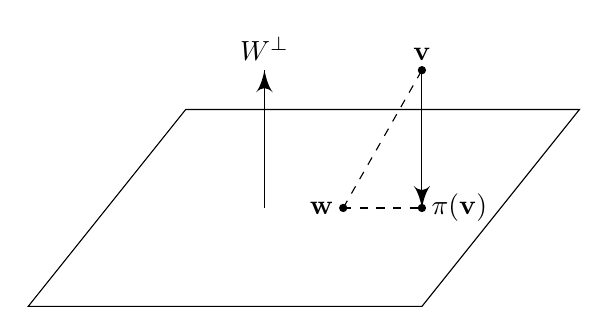
\begin{tikzpicture}
          \draw (0, 0) -- (5, 0) -- (7, 2.5) -- (2, 2.5) -- cycle;
          \draw [->] (3, 1.25) -- (3, 3) node [above] {$W^\perp$};
          \draw [dashed] (4, 1.25) node [left] {$\mathbf{w}$} -- (5, 3) node [above] {$\mathbf{v}$};
          \draw [->] (5, 3) -- (5, 1.25) node [right] {$\pi(\mathbf{v})$};
          \draw [dashed] (4, 1.25) -- (5, 1.25);
          \node at (5, 3) [circ] {};
          \node at (4, 1.25) [circ] {};
          \node at (5, 1.25) [circ] {};
        \end{tikzpicture}
      \end{center}
  \end{enumerate}
\end{prop}

\begin{proof}\leavevmode
  \begin{enumerate}
    \item Let $\mathbf{v} \in V$, and define
      \[
        \mathbf{w} = \sum_{i = 1} (\mathbf{e}_i, \mathbf{v}) \mathbf{e}_i.
      \]
      We want to show this is $\pi(\mathbf{v})$. We need to show $\mathbf{v} - \mathbf{w} \in W^\perp$. We can compute
      \[
        (\mathbf{e}_j, \mathbf{v} - \mathbf{w}) = (\mathbf{e}_j, \mathbf{v}) + \sum_{i = 1}^k (\mathbf{e}_i, \mathbf{v}) (\mathbf{e}_j, \mathbf{e}_i) = 0.
      \]
      So $\mathbf{v} - \mathbf{w}$ is orthogonal to every basis vector in $\mathbf{w}$, ie. $\mathbf{v} - \mathbf{w} \in W^\perp$.So
      \[
        \pi(\mathbf{v}) = \pi(\mathbf{w}) + \pi(\mathbf{v} - \mathbf{w}) = \mathbf{w}
      \]
      as required.
    \item This is just Pythagoras' theorem. Note that if $\mathbf{x}$ and $\mathbf{y}$ are orthogonal, then
      \begin{align*}
        \|\mathbf{x} + \mathbf{y}\|^2 &= (\mathbf{x} + \mathbf{y}, \mathbf{x} + \mathbf{y}) \\
        &= (\mathbf{x}, \mathbf{x}) + (\mathbf{x}, \mathbf{y}) + (\mathbf{y}, \mathbf{x}) + (\mathbf{y}. \mathbf{y})\\
        &= \|\mathbf{x}\|^2 + \|\mathbf{y}\|^2.
      \end{align*}
      We apply this to our projection. For any $\mathbf{w} \in W$, we have
      \[
        \|\mathbf{v} - \mathbf{w}\|^2 = \|\mathbf{v} - \pi (\mathbf{v})\|^2 + \|\pi(\mathbf{v}) - \mathbf{w}\|^2 \geq \|\mathbf{v} - \pi(\mathbf{v})\|^2
      \]
      with equality if and only if $\|\pi(\mathbf{v}) - \mathbf{w}\| = 0$, ie. $\pi(\mathbf{v}) = \mathbf{w}$.
  \end{enumerate}
\end{proof}

\subsection{Adjoints, orthogonal and unitary maps}
\subsubsection*{Adjoints}
\begin{lemma}
  Let $V$ and $W$ be finite-dimensional inner product spaces and $\alpha: V \to W$ is a linear map. Then there exists a unique linear map $\alpha^*: W \to V$ such that
  \[
    (\alpha \mathbf{v}, \mathbf{w}) = (\mathbf{v}, \alpha^* \mathbf{w})\tag{$*$}
  \]
  for all $\mathbf{v} \in V$, $\mathbf{w} \in W$.
\end{lemma}

\begin{proof}
  There are two parts. We have to prove existence and uniqueness. We'll first proof it concretely using matrices, and then provide a conceptual reason of what this means.

  Let $(\mathbf{v}_1, \cdots, \mathbf{v}_n)$ and $(\mathbf{w}_1, \cdots, \mathbf{w}_m)$ be orthonormal basis for $V$ and $W$. Suppose $\alpha$ is represented by $A$.

  To show uniqueness, suppose $\alpha^*: W \to V$ satisfies $(\alpha \mathbf{v}, \mathbf{w}) = (\mathbf{v}, \alpha^* \mathbf{w})$ for all $\mathbf{v} \in V$, $\mathbf{w} \in W$, then for all $i, j$, by definition, we know
  \begin{align*}
    (\mathbf{v}_i, \alpha^*(\mathbf{w}_j)) &= (\alpha(\mathbf{v}_i), \mathbf{w}_j) \\
    &= \left(\sum_k A_{ki} \mathbf{w}_k, \mathbf{w}_j\right)\\
    &= \sum_k \bar{A}_{ki} (\mathbf{w}_k, \mathbf{w}_j) = \bar{A}_{ji}.
  \end{align*}
  So we get
  \[
    \alpha^*(\mathbf{w}_j) = \sum_i (\mathbf{v}_i, \alpha^*(\mathbf{w}_j)) \mathbf{v}_i = \sum_i \bar{A}_{ji} \mathbf{v}_i.
  \]
  Hence $\alpha^*$ must be represented by $A^\dagger$. So $\alpha^*$ is unique.

  To show existence, all we have to do is to show $A^\dagger$ indeed works. Now let $\alpha^*$ be represented by $A^\dagger$. We can compute the two sides of $(*)$ for arbitrary $\mathbf{v}, \mathbf{w}$. We have
  \begin{align*}
    \left(\alpha\left(\sum \lambda_i \mathbf{v}_i\right), \sum \mu_j \mathbf{w}_j\right) &= \sum_{i, j} \bar{\lambda}_i \mu_j (\alpha(\mathbf{v}_i), \mathbf{w}_j)\\
    &= \sum_{i, j} \bar{\lambda}_i \mu_j \left(\sum_k A_{ki} \mathbf{w}_k, \mathbf{w}_j\right)\\
    &= \sum_{i, j} \bar{\lambda}_i \bar{A}_{ji} \mu_j.
  \end{align*}
  We can compute the other side and get
  \begin{align*}
    \left(\sum \lambda_i \mathbf{v}_i, \alpha^*\left(\sum \mu_j \mathbf{w}_j\right)\right) &= \sum_{i, j} \bar{\lambda}_i \mu_j \left(\mathbf{v}_i, \sum_k A^{\dagger} A_{kj} \mathbf{v}_k\right)\\
    &= \sum_{i, j} \bar{\lambda}_i \bar{A}_{ji} \mu_j.
  \end{align*}
  So done.
\end{proof}
What does this mean, conceptually? Note that the inner product $V$ defines an isomorphism $V \to \bar{V}^*$ by $\mathbf{v} \mapsto (\ph,\mathbf{v})$. Similarly, we have an isomorphism $W \to \bar{W}^*$. We can then put them in the following diagram:
\[
  \begin{tikzcd}
    V \ar[r, "\alpha"] \ar[d, "\cong"] & W \ar[d, "\cong"]\\
    \bar{V}^* & \bar{W}^* \ar[l, dashed, "\alpha^*"]
  \end{tikzcd}
\]
Then $\alpha^*$ is what fills in the dashed arrow. So $\alpha^*$ is in some sense the ``dual'' of the map $\alpha$.

\begin{defi}[Adjoint]
  We call the map $\alpha^*$ the \emph{adjoint} of $\alpha$.
\end{defi}
We have just seen that if $\alpha$ is represented by $A$ with respect to some orthonormal bases, then $\alpha^*$ is represented by $A^\dagger$.

\begin{defi}[Self-adjoint]
  Let $V$ be an inner product space, and $\alpha \in \End(V)$. Then $\alpha$ is \emph{self-adjoint} if $\alpha = \alpha^*$, ie.
  \[
    (\alpha(\mathbf{v}), \mathbf{w}) = (\mathbf{v}, \alpha(\mathbf{w}))
  \]
  for all $\mathbf{v}, \mathbf{w}$.
\end{defi}
Thus if $V = \R^n$ with the usual inner product, then $A \in \Mat_n(\R)$ is self-adjoint if and only if it is symmetric, ie. $A = A^T$. If $V = \C^n$ with the usual inner product, then $A \in \Mat_n(\C)$ is self-adjoint if and only if $A$ is Hermitian, ie. $A = A^\dagger$.

Self-adjoint endomorphisms are important, as you may have noticed from IB Quantum Mechanics. We will later see that these have real eigenvalues with an orthonormal basis of eigenvectors.

\subsubsection*{Orthogonal maps}
Another important class of endomorphisms is those that preserve lengths. We will first do this for real vector spaces, since the real and complex versions have different names.
\begin{defi}[Orthogonal endomorphism]
  Let $V$ be a real inner product space. Then $\alpha \in \End(V)$ is \emph{orthogonal} if
  \[
    (\alpha(\mathbf{v}), \alpha(\mathbf{w})) = (\mathbf{v}, \mathbf{w})
  \]
  for all $\mathbf{v}, \mathbf{w} \in V$.
\end{defi}
By the polarization identity, $\alpha$ is orthogonal if and only if $\|\alpha(\mathbf{v})\| = \|\mathbf{v}\|$ for all $\mathbf{v} \in V$.

A real square matrix (as an endomorphism of $\R^n$ with the usual inner product) is orthogonal if and only if its columns are an orthonormal set.

There is also an alternative way of characterizing these orthogonal maps.

\begin{lemma}
  Let $V$ be a finite-dimensional space and $\alpha \in \End(V)$. Then $\alpha$ is orthogonal if and only if $\alpha^{-1} = \alpha^*$.
\end{lemma}

\begin{proof}
  $(\Leftarrow)$ Suppose $\alpha^{-1} = \alpha^*$. If $\alpha^{-1} = \alpha^*$, then
  \[
    (\alpha \mathbf{v}, \alpha \mathbf{v}) = (\mathbf{v}, \alpha^* \alpha \mathbf{v}) = (\mathbf{v}, \alpha^{-1} \alpha \mathbf{v}) = (\mathbf{v}, \mathbf{v}).
  \]
  $(\Rightarrow)$ If $\alpha$ is orthogonal and $(\mathbf{v}_1, \cdots, \mathbf{v}_n)$ is an orthonormal basis for $V$, then for $1 \leq i, j \leq n$, we have
  \[
    \delta_{ij} = (\mathbf{v}_i, \mathbf{v}_j) = (\alpha \mathbf{v}_i, \alpha \mathbf{v}_j) = (\mathbf{v}_i, \alpha^* \alpha \mathbf{v}_j).
  \]
  So we know
  \[
    \alpha^* \alpha (\mathbf{v}_j) = \sum_{i = 1}^n (\mathbf{v}_i, \alpha^* \alpha \mathbf{v}_j)) \mathbf{v}_i = \mathbf{v}_j.
  \]
  So by linearity of $\alpha^* \alpha$, we know $\alpha^* \alpha = \id_V$. So $\alpha^* = \alpha^{-1}$.
\end{proof}

\begin{cor}
  $\alpha \in \End(V)$ is orthogonal if and only if $\alpha$ is represented by an orthogonal matrix, ie. a matrix $A$ such that $A^T A = AA^T = I$, with respect to any orthonormal basis.
\end{cor}

\begin{proof}
  Let $(\mathbf{e}_1, \cdots, \mathbf{e}_n)$ be an orthonormal basis for $V$. Then suppose $\alpha$ is represented by $A$. So $\alpha^*$ is represented by $A^T$. Then $A^* = A^{-1}$ if and only if $AA^T = A^T A = I$.
\end{proof}

\begin{defi}[Orthogonal group]
  Let $V$ be a real inner product space. Then the \emph{orthogonal group} of $V$ is
  \[
    \Or(V) = \{\alpha \in \End(V): \alpha\text{ is orthogonal}\}.
  \]
\end{defi}
It follows from the fact that $\alpha^* = \alpha^{-1}$ that $\alpha$ is invertible, and it is clear from definition that $\Or(V)$ is closed under multiplication and inverses. So this is indeed a group.

\begin{prop}
  Let $V$ be a finite-dimensional real inner product space and $(\mathbf{e}_1, \cdots, \mathbf{e}_n)$ is an orthonormal basis of $V$. Then there is a bijection
  \begin{align*}
    \Or(V) &\to \{\text{orthonormal basis for }V\}\\
    \alpha &\mapsto (\alpha(\mathbf{e}_1, \cdots, \mathbf{e}_n)).
  \end{align*}
\end{prop}
This is analogous to our result for general vector spaces and general bases, where we replace $\Or(V)$ with $\GL(V)$.

\begin{proof}
  Same as the case for general vector spaces and general bases.
\end{proof}

\subsubsection*{Unitary maps}
We are going to study the complex version of orthogonal maps, known as \emph{unitary maps}. The proofs are almost always identical to the real case, and we will not write the proofs again.

\begin{defi}[Unitary map]
  Let $V$ be a finite-dimensional complex vector space. Then $\alpha \in \End(V)$ is \emph{unitary} if
  \[
    (\alpha(\mathbf{v}), \alpha(\mathbf{w})) = (\mathbf{v}, \mathbf{w})
  \]
  for all $\mathbf{v}, \mathbf{w} \in V$.
\end{defi}
By the polarization identity, $\alpha$ is unitary if and only if $\|\alpha(\mathbf{v})\| = \|\mathbf{v}\|$ for all $\mathbf{v} \in V$.

\begin{lemma}
  Let $V$ be a finite dimensional complex inner product space and $\alpha \in \End(V)$. Then $\alpha$ is unitary if and only if $\alpha$ is invertible and $\alpha^* = \alpha^{-1}$.
\end{lemma}

\begin{cor}
  $\alpha \in \End(V)$ is unitary if and only if $\alpha$ is represented by a unitary matrix $A$ with respect to any orthonormal basis, ie. $A^{-1} = A^\dagger$.
\end{cor}

\begin{defi}[Unitary group]
  Let $V$ be a finite-dimensional complex inner product space. Then the \emph{unitary group} of $V$ is
  \[
    U(V) = \{\alpha \in \End(V): \alpha\text{ is unitary}\}.
  \]
\end{defi}

\begin{prop}
  Let $V$ be a finite-dimensional complex inner product space. Then there is a bijection
  \begin{align*}
    U(V) &\to \{\text{orthonormal basis of } V\}\\
    \alpha &\mapsto \{\alpha(\mathbf{e}_1), \cdots, \alpha (\mathbf{e}_n)\}.
  \end{align*}
\end{prop}

\subsection{Spectral theory}
We are going to classify matrices in inner product spaces. Recall that for general vector spaces, what we effectively did was to find the orbits of the conjugation action of $\GL(V)$ on $\Mat_n(\F)$. If we have inner product spaces, we will want to look at the action of $O(V)$ or $U(V)$ on $\Mat_n(\F)$. In a more human language, instead of allowing arbitrary basis transformations, we only allow transforming between orthonormal basis.

We are not going to classify all endomorphisms, but just self-adjoint and orthogonal/unitary ones.

\begin{lemma}
  Let $V$ be a finite-dimensional inner product space, and $\alpha \in \End(V)$ self-adjoint. Then
  \begin{enumerate}
    \item $\alpha$ has a real eigenvalue, and all eigenvalues of $\alpha$ are real.
    \item Eigenvectors of $\alpha$ with distinct eigenvalues are orthogonal.
  \end{enumerate}
\end{lemma}

\begin{proof}
  We are going to do real and complex cases separately.
  \begin{enumerate}
    \item Suppose first $V$ is a complex inner product space. Then by the fundamental theorem of algebra, $\alpha$ has an eigenvalue, say $\lambda$. We pick $\mathbf{v} \in V\setminus \{0\}$ such that $\alpha \mathbf{v} = \lambda \mathbf{v}$. Then
      \[
        \bar{\lambda}(\mathbf{v}, \mathbf{v}) = (\lambda \mathbf{v}, \mathbf{v}) = (\alpha \mathbf{v}, \mathbf{v}) = (\mathbf{v}, \alpha \mathbf{v}) = (\mathbf{v}, \lambda \mathbf{v}) = \lambda (\mathbf{v}, \mathbf{v}).
      \]
      Since $\mathbf{v}\not= \mathbf{0}$, we know $(\mathbf{v}, \mathbf{v})\not= 0$. So $\lambda = \bar{\lambda}$.

      For the real case, we pretend we are in the complex case. Let $\mathbf{e}_1, \cdots, \mathbf{e}_n$ be an orthonormal basis for $V$. Then $\alpha$ is represented by a symmetric matrix $A$ (with respect to this basis). Since real symmetric matrices are Hermitian viewed as complex matrices, this gives a self-adjoint endomorphism of $\C^n$. By the complex case, $A$ has real eigenvalues only. But the eigenvalues of $A$ are the eigenvalues of $\alpha$ and $M_A(t) = M_\alpha(t)$. So done.

      Alternatively, we can prove this without reducing to the complex case. We know every irreducible factor of $M_\alpha(t)$ in $\R[t]$ must have degree $1$ or $2$, since the roots are either real or come in complex conjugate pairs. Suppose $f(t)$ were an irreducible factor of degree $2$. Then
      \[
        \left(\frac{m_\alpha}{f}\right)(\alpha) \not= 0
      \]
      since it has degree less than the minimal polynomial. So there is some $\mathbf{v} \in V$ such that
      \[
        \left(\frac{M_\alpha}{f}\right)(\alpha)(\mathbf{v}) \not= \mathbf{0}.
      \]
      So it must be that $f(\alpha)(\mathbf{v}) = \mathbf{0}$. Let $U = \bra \mathbf{v}, \alpha (\mathbf{v})\ket$. Then this is an $\alpha$-invariant subspace of $V$ since $f$ has degree $2$.

      Now $\alpha|_U \in \End(U)$ is self-adjoint. So if $(\mathbf{e}_1, \mathbf{e}_2)$ is an orthonormal basis of $U$, then $\alpha$ is represented by a real symmetric matrix, say
      \[
        \begin{pmatrix}
          a & b\\
          b & a
        \end{pmatrix}
      \]
      But then $\chi_{\alpha|_U}(t) = (t - a)^2 - b^2$, which has real roots, namely $a \pm b$. This is a contradiction, since $M_{\alpha|_U} = f$, but $f$ is irreducible.
    \item Now suppose $\alpha \mathbf{v} = \lambda \mathbf{v}$, $\alpha \mathbf{w} = \mu \mathbf{w}$ and $\lambda \not= \mu$. We need to show $(\mathbf{v}, \mathbf{w}) = 0$. We know
      \[
        (\alpha \mathbf{v}, \mathbf{w}) = (\mathbf{v}, \alpha \mathbf{w})
      \]
      by definition. This then gives
      \[
        \lambda (\mathbf{v}, \mathbf{w}) = \mu (\mathbf{v}, \mathbf{w})
      \]
      Since $\lambda \not= \mu$, we must have $(\mathbf{v}, \mathbf{w}) = 0$.
  \end{enumerate}
\end{proof}

\begin{thm}
  Let $V$ be a finite-dimensional inner product space, and $\alpha \in \End(V)$ self-adjoint. Then $V$ has an orthonormal basis of eigenvectors of $\alpha$.
\end{thm}

\begin{proof}
  By the previous lemma, $\alpha$ has a real eigenvalue, say $\lambda$. Then we can find an eigenvector $\mathbf{v} \in V\setminus \{0\}$ such that $\alpha \mathbf{v} = \lambda \mathbf{v}$.

  Let $U = \bra \mathbf{v}\ket ^\perp$. Then we can write
  \[
    V = \bra \mathbf{v}\ket \perp U.
  \]
  We now want to prove $\alpha$ sends $U$ into $U$. Suppose $\mathbf{u} \in U$. Then
  \[
    (\mathbf{v}, \alpha (\mathbf{u})) = (\alpha \mathbf{v}, \mathbf{u}) = \lambda (\mathbf{v}, \mathbf{u}) = 0.
  \]
  So $\alpha (\mathbf{u}) \in \bra \mathbf{v}\ket^\perp = U$. So $\alpha|_U \in \End(U)$ and is self-adjoint.

  By induction on $\dim V$, $U$ has an orthonormal basis $(\mathbf{v}_2, \cdots, \mathbf{v}_n)$ of $\alpha$ eigenvectors. Now let
  \[
    \mathbf{v}_1 = \frac{\mathbf{v}}{\|\mathbf{v}\|}.
  \]
  Then $(\mathbf{v}_1, \mathbf{v}_2, \cdots, \mathbf{v}_n)$ is an orthonormal basis of eigenvectors for $\alpha$.
\end{proof}

\begin{cor}
  Let $V$ be a finite-dimensional vector space and $\alpha$ self-adjoint. Then $V$ is the orthogonal (internal) direct sum of its $\alpha$-eigenspaces.
\end{cor}

\begin{cor}
  Let $A \in \Mat_n(\R)$ be symmetric. Then there exists an orthogonal matrix $P$ such that $P^TAP = P^{-1}AP$ is diagonal.
\end{cor}

\begin{proof}
  Let $(\ph, \ph)$ be the standard inner product on $\R^n$. Then $A$ is self-adjoint as an endomorphism of $\R^n$. So $\R^n$ has an orthonormal basis of eigenvectors for $A$, say $(\mathbf{v}_1, \cdots, \mathbf{v}_n)$. Taking $P = (\mathbf{v}_1\; \mathbf{v}_2\; \cdots \; \mathbf{v}_n)$ gives the result.
\end{proof}

\begin{cor}
  Let $V$ be a finite-dimensional real inner product space and $\psi: V\times V \to \R$ a symmetric bilinear form. Then there exists an orthonormal basis $(\mathbf{v}_1, \cdots, \mathbf{v}_n)$ for $V$ with respect to which $\psi$ is represented by a diagonal matrix.
\end{cor}

\begin{proof}
  Let $(\mathbf{u}_1, \cdots, \mathbf{u}_n)$ be any orthonormal basis for $V$. Then $\psi$ is represented by a symmetric matrix $A$. Then there exists an orthogonal matrix $P$ such that $P^T AP$ is diagonal. Now let $\mathbf{v}_i = \sum P_{ki} \mathbf{u}_k$. Then $(\mathbf{v}_1, \cdots, \mathbf{v}_n)$ is an orthonormal basis since
  \begin{align*}
    (\mathbf{v}_i, \mathbf{v}_j) &= \left(\sum P_{ki} \mathbf{u}_k, \sum P_{\ell j} \mathbf{u}_\ell\right) \\
    &= \sum P_{ik}^T (\mathbf{u}_k, \mathbf{u}_\ell) P_{\ell j}\\
    &= [P^T P]_{ij}\\
    &= \delta_{ij}.
  \end{align*}
  Also, $\psi$ is represented by $P^T AP$ with respect to $(\mathbf{v}_1, \cdots, \mathbf{v}_n)$.
\end{proof}
Note that the diagonal values of $P^T AP$ are just the eigenvalues of $A$. So the signature of $\psi$ is just the number of positive eigenvalues of $A$ minus the number of negative eigenvalues of $A$.

\begin{cor}
  Let $V$ be a finite-dimensional real vector space and $\phi, \psi$ symmetric bilinear forms on $V$ such that $\phi$ is positive-definite. Then we can find a basis $(\mathbf{v}_1, \cdots, \mathbf{v}_n)$ for $V$ such that both $\phi$ and $\psi$ are represented by diagonal matrices with respect to this basis.
\end{cor}

\begin{proof}
  We use $\phi$ to define an inner product. Choose an orthonormal basis for $V$ (equipped with $\phi$) $(\mathbf{v}_1, \cdots, \mathbf{v}_n)$ with respect to which $\psi$ is diagonal. Then $\phi$ is represented by $I$ with respect to this basis, since $\psi(\mathbf{v}_i, \mathbf{v}_j) = \delta_{ij}$. So done.
\end{proof}

\begin{cor}
  If $A, B \in \Mat_n(\R)$ are symmetric and $A$ is positive definitive (ie. $\mathbf{v}^T A \mathbf{v} > 0$ for all $\mathbf{v} \in \R^n \setminus \{0\}$). Then there exists an invertible matrix $Q$ such that $Q^T AQ$ and $Q^T BQ$ are both diagonal.
\end{cor}

We can deduce similar results for complex finite-dimensional vector spaces, with the same proofs. In particular,
\begin{prop}\leavevmode
  \begin{enumerate}
    \item If $A \in \Mat_n(\C)$ is Hermitian, then there exists a unitary matrix $U \in \Mat_n(\C)$ such that
      \[
        U^{-1}AU = U^\dagger AU
      \]
      is diagonal.
    \item If $\psi$ is a Hermitian form on a finite-dimensional complex inner product space $V$, then there is an orthonormal basis for $V$ diagonalizing $\psi$.
    \item If $\phi, \psi$ are Hermitian forms on a finite-dimensional complex vector space and $\phi$ is positive definite, then there exists a basis for which $\phi$ and $\psi$ are diagonalized.
    \item Let $A, B \in \Mat_n(\C)$ be Hermitian, and $A$ positive definitive (ie. $\mathbf{v}^\dagger A \mathbf{v} > 0$ for $\mathbf{v} \in V \setminus \{0\}$). Then there exists some invertible $Q$ such that $Q^\dagger AQ$ and $Q^\dagger BQ$ are diagonal.
  \end{enumerate}
\end{prop}

That's all for self-adjoint matrices. How about unitary matrices?
\begin{thm}
  Let $V$ be a finite-dimensional complex vector space and $\alpha \in U(V)$ be unitary. Then $V$ has an orthonormal basis of $\alpha$ eigenvectors.
\end{thm}

\begin{proof}
  By the fundamental theorem of algebra, there exists $\mathbf{v} \in V\setminus \{0\}$ and $\lambda \in \C$ such that $\alpha \mathbf{v} = \lambda \mathbf{v}$. Now consider $W = \bra \mathbf{v}\ket^\perp$. Then
  \[
    V = W \perp \bra \mathbf{v}\ket.
  \]
  We want to show $\alpha$ restricts to a (unitary) endomorphism of $W$. Let $\mathbf{w} \in W$. We need to show $\alpha(\mathbf{w})$ is orthogonal to $\mathbf{v}$. We have
  \[
    (\alpha \mathbf{w}, \mathbf{v}) = (\mathbf{w}, \alpha^{-1}\mathbf{v}) = (\mathbf{w}, \lambda^{-1} \mathbf{v}) = 0.
  \]
  So $\alpha(\mathbf{w}) \in W$ and $\alpha|_W \in \End(W)$. Also, $\alpha|_W$ is unitary since $\alpha$ is. So by induction on $\dim V$, $W$ has an orthonormal basis of $\alpha$ eigenvectors. If we add $\mathbf{v}/\|\mathbf{v}\|$ to this basis, we get an orthonormal basis of $V$ itself comprised of $\alpha$ eigenvectors.
\end{proof}
This theorem and the analogous one for self-adjoint endomorphisms have a common generalization, at least for complex inner product spaces. The key fact that leads to the existence of an orthonormal basis of eigenvectors is that $\alpha$ and $\alpha^*$ commute. This is clearly a necessary condition, since if $\alpha$ is diagonalizable, then $\alpha^*$ is diagonal in the same basis (since it is just the transpose (and conjugate)), and hence they commute. It turns out this is also a sufficient condition, as you will show in example sheet 4.

However, we cannot generalize this in the real orthogonal case. For example,
\[
  \begin{pmatrix}
    \cos \theta & \sin \theta\\
    - \sin \theta & \cos \theta
  \end{pmatrix} \in O(\R^2)
\]
cannot be diagonalized (if $\theta \not\in \pi \Z$). However, in example sheet 4, you will find a classification of $O(V)$, and you will see that the above counterexample is the worst that can happen in some sense.
\end{document}
